%%%%%%%%%%%%%%%%%%%%%%%%%%%%%%%%%%%%%%%%%%%%%%%%%%%%%%%%%%%%%%%%%%%%%%%%%%%%%%%%%%%%%%%%%%%%%%%%%%%%%%%%%%%
%                                           PACKAGES                                                      %
%%%%%%%%%%%%%%%%%%%%%%%%%%%%%%%%%%%%%%%%%%%%%%%%%%%%%%%%%%%%%%%%%%%%%%%%%%%%%%%%%%%%%%%%%%%%%%%%%%%%%%%%%%%
\documentclass[12pt, fleqn]{article}
\usepackage{amsmath, amsfonts, amsthm, amssymb, graphicx, enumitem, mathtools, MnSymbol, relsize, cancel}
\usepackage{siunitx}
\DeclareSIUnit\angstrom{\text{\AA}}
\usepackage{pdfpages}
\usepackage{graphicx}
\usepackage[utf8]{inputenc}
\usepackage{biblatex}
\usepackage{pythontex}
\usepackage{listings}
\usepackage[pdftex,pdfpagelabels,bookmarks,hyperindex,hyperfigures]{hyperref}
\hypersetup{colorlinks=true,allcolors=blue}
\usepackage{hypcap}
\usepackage{float}
\usepackage{geometry}
\geometry{margin=1in}
%%%%%%%%%%%%%%%%%%%%%%%%%%%%%%%%%%%%%%%%%%%%%%%%%%%%%%%%%%%%%%%%%%%%%%%%%%%%%%%%%%%%%%%%%%%%%%%%%%%%%%%%%%%
%                                           REFERENCE FILE                                                %
%%%%%%%%%%%%%%%%%%%%%%%%%%%%%%%%%%%%%%%%%%%%%%%%%%%%%%%%%%%%%%%%%%%%%%%%%%%%%%%%%%%%%%%%%%%%%%%%%%%%%%%%%%%
\usepackage[export]{adjustbox}
\graphicspath{{images/}}
%%%%%%%%%%%%%%%%%%%%%%%%%%%%%%%%%%%%%%%%%%%%%%%%%%%%%%%%%%%%%%%%%%%%%%%%%%%%%%%%%%%%%%%%%%%%%%%%%%%%%%%%%%%
%                                          PREPARE TITLE AND ABSTRACT                                     %
%%%%%%%%%%%%%%%%%%%%%%%%%%%%%%%%%%%%%%%%%%%%%%%%%%%%%%%%%%%%%%%%%%%%%%%%%%%%%%%%%%%%%%%%%%%%%%%%%%%%%%%%%%%
\title {
    \normalsize{UC Berkeley}\\
    \large{{EE140: Analog Integrated Circuit Devices\\Fall 2022\\Professor Ricky Muller\\}}
    \vspace{0.5ex}
    \Huge{Lab 1 Report}
    \vspace{0.5ex}
}
\addbibresource{references.bib}
\author{Tarik Fawal}
\date{4 October 2022}
\usepackage{array}
\newcolumntype{C}[1]{>{\centering\arraybackslash}m{#1}}
\newcolumntype{N}{@{}m{0pt}@{}}
\begin{document}
%%%%%%%%%%%%%%%%%%%%%%%%%%%%%%%%%%%%%%%%%%%%%%%%%%%%%%%%%%%%%%%%%%%%%%%%%%%%%%%%%%%%%%%%%%%%%%%%%%%%%%%%%%%
%                                           GENERATE TITLE                                                %
%%%%%%%%%%%%%%%%%%%%%%%%%%%%%%%%%%%%%%%%%%%%%%%%%%%%%%%%%%%%%%%%%%%%%%%%%%%%%%%%%%%%%%%%%%%%%%%%%%%%%%%%%%%
\maketitle
\tableofcontents
\flushbottom
    \section*{Preface}
        \textit{\emph{This lab report was created using \LaTeX.  The answers to questions were obtained through the course website, notes, textbook, and lecture videos.  I pledge that I have not plagiarized my solutions in any way, and the work presented here is my own.  References to any sources of material used in the solutions to this lab report are included at the end of this document.}}
%%%%%%%%%%%%%%%%%%%%%%%%%%%%%%%%%%%%%%%%%%%%%%%%%%%%%%%%%%%%%%%%%%%%%%%%%%%%%%%%%%%%%%%%%%%%%%%%%%%%%%%%%%%
%                                               PART 1                                                    %
%%%%%%%%%%%%%%%%%%%%%%%%%%%%%%%%%%%%%%%%%%%%%%%%%%%%%%%%%%%%%%%%%%%%%%%%%%%%%%%%%%%%%%%%%%%%%%%%%%%%%%%%%%%
\newpage
\section{Part I}
%%%%%%%%%%%%%%%%%%%%%%%%%%%%%%%%%%%%%%%%%%%%%%%%%%%%%%
%                       TASK A                       %
%%%%%%%%%%%%%%%%%%%%%%%%%%%%%%%%%%%%%%%%%%%%%%%%%%%%%%
\subsection{Task A}

There are two tasks in this part. For both parts, assume the following parameters for the transistor when doing hand calculations and simulations:

\begin{table}[H]
\centering
\setlength{\tabcolsep}{20pt}
\renewcommand{\arraystretch}{1.5}
\begin{tabular}{|l|c|c|}
    \hline
    \textbf{\textit{\textbf{Parameter}}}  &  \textit{\textbf{NMOS}} & \textit{\textbf{PMOS}}\\
    \hline
    \textit{Model Level} & 3 (in HSPICE) & 3 (in HSPICE)\\
    \hline
    \textit{VTO} & $0.8\,V$ & $-0.8\,$\\
    \hline
    \textit{KP} & $90\,\mu A/V^2$ & $30\,\mu A/V^2$\\
    \hline
    \textit{GAMMA} & $0.8\,\sqrt{V}$ & $0.4\,\sqrt{V}$\\
    \hline
    \textit{LAMBDA} & $0.01\,V^{-1}$ & $0.02\,V^{-1}$\\
    \hline
    \textit{TOX} & $200\,\text{AA}$ & $200\,\text{AA}$\\
    \hline
    \textit{XJ} & $0.5\,\mu m$ & $0.5\,\mu m$\\
    \hline
    \textit{LD} & $0.3\,\mu m$ & $0.3\,\mu m$\\
    \hline
    \textit{PHI} & $0.7\,V$ & $0.6\,V$\\
    \hline
    \textit{NSUB} & $\num{3.33e16}\,cm^{-3}$ & $\num{3.33e15}\,cm^{-3}$\\
    \hline
    \textit{RSH} & $0\,\Omega$ & $0\,\Omega$\\
    \hline
    \textit{CGSO} & $500\,pF/m$ & $500\,pF/m$\\
    \hline
    \textit{CGDO} & $500\,pF/m$ & $500\,pF/m$\\
    \hline
    \textit{CGBO} & $0\,F/m$ & $0\,F/m$\\
    \hline
    \textit{CJ} & $300\,\mu F/m^2$ & $300\,\mu F/m^2$\\
    \hline
    \textit{MJ} & $0.5$ & $0.5$\\
    \hline
    \textit{CJSW} & $0\,F/m$ & $0\,F/m$\\
    \hline
    \textit{MJSW} & $0.33$ & $0.33$\\
    \hline
\end{tabular}
\caption{Process / SPICE parameters for NMOS / PMOS transistors.
\label{tab:proc_param}} 
\end{table}

\newpage\noindent
\textbf{\emph{Given: }} A saturated $NMOS$ load degenerated-source amplifier shown in \textit{Fig. 1} below.

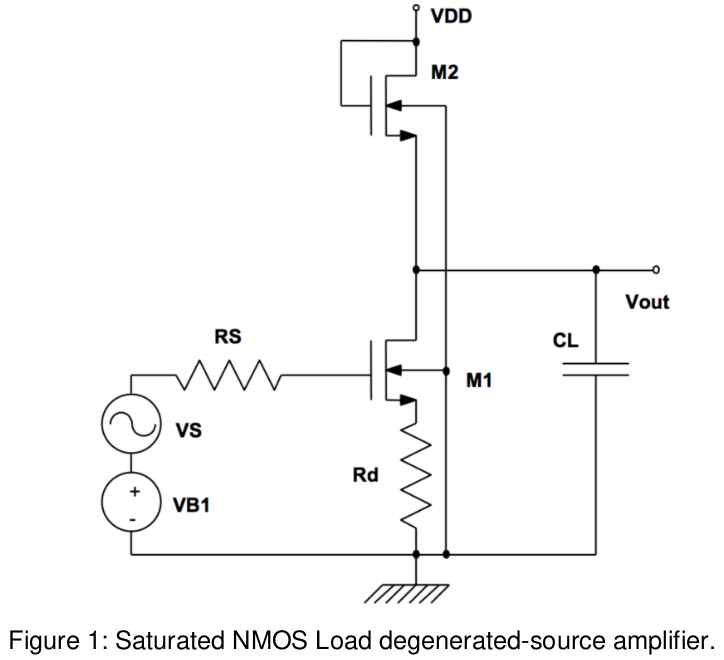
\includegraphics[scale=0.35, center]{p1nmos.PNG}\\

The amplifier has the following parameters:

\begin{table}[H]
\centering
\setlength{\tabcolsep}{20pt}
\renewcommand{\arraystretch}{1.5}
\begin{tabular}{|l|c|}
    \hline
    $V_{DD}$ & $5\,V$\\
    \hline
    $V_{B1}$ & $1.1\,V$\\
    \hline
    $R_D$ & $0\,\Omega$\\
    \hline
    $R_S$ & $5\,k\Omega$\\
    \hline
    $C_L$ & $2.5\,pF$\\
    \hline
    $\left(\frac{W}{L}_1\right)$ & $\frac{50\,\mu m}{5\,\mu m}$\\
    \hline
    $\left(\frac{W}{L}_2\right)$ & $\frac{10\,\mu m}{90\,\mu m}$\\
    \hline
\end{tabular}
\caption{Given amplifier parameters.
\label{tab:amp_param}} 
\end{table}

\noindent
\textbf{\emph{Find: }}\\[0.25cm]
\noindent
Determine the small-signal voltage gain $\frac{v_{out}}{v_s}$, the upper cutoff frequency (or bandwidth), and the output resistance of the amplifier using BOTH hand calculation and simulation. You should show the plot of the magnitude of the gain (in $dB$ or $V/V$ log scale) vs. log-scale frequency for this amplifier. Note that you can make any reasonable approximations in your hand calculations.  If the simulated and calculated results do not agree, you should discuss the reasons. Also determine the maximum output voltage swing that this amplifier can deliver. You can use simulation only for this part.

\newpage\noindent
\textbf{\emph{Solution: }}

%%%%%%%%%%%%%%%%%%%%%%%%%%%%%%%%%%%%%%%%
%            HAND CALCULATIONS         %
%%%%%%%%%%%%%%%%%%%%%%%%%%%%%%%%%%%%%%%%
\subsubsection{Hand Calculations}

For the hand calculations we will be ignoring the body effect and channel length modulation.  We will only take into account the time constants from $C_{GD}$, $C_{GS}$, and $C_L$ when determining the overall bandwidth.  Below is the work done for all hand calculations of this amplifier:\\[1cm]
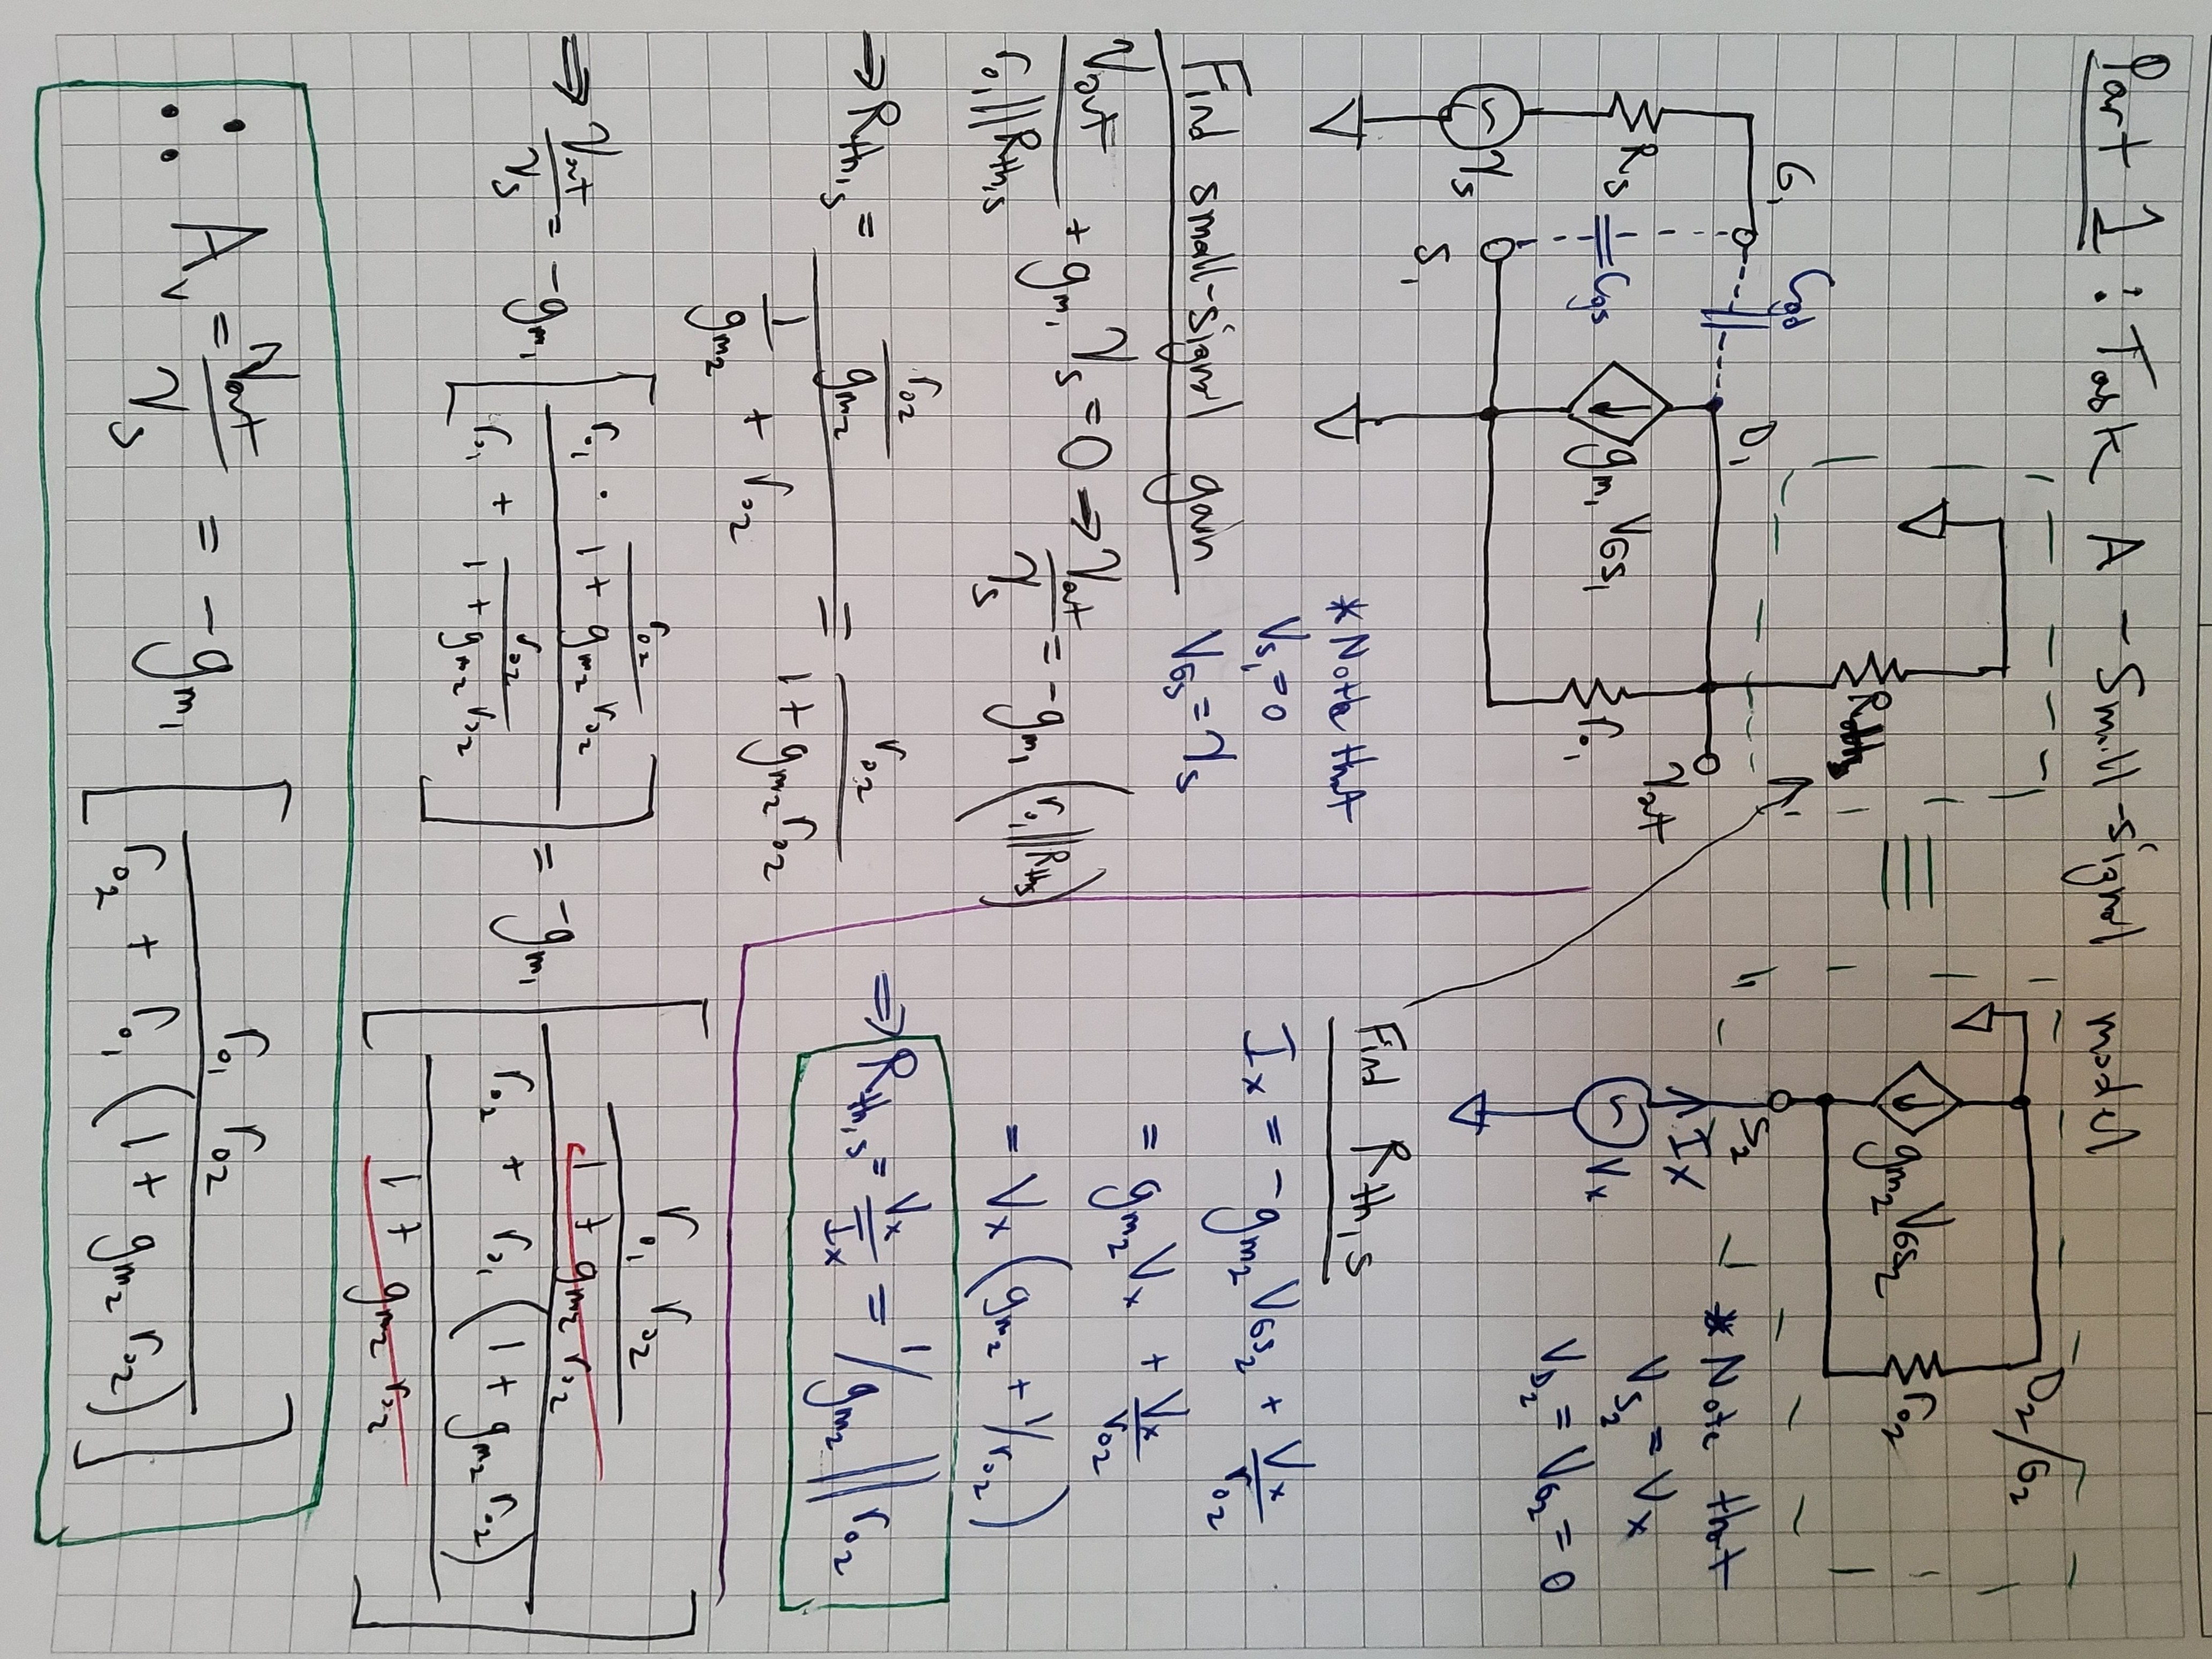
\includegraphics[scale=0.125, angle=90, center]{p1_1.jpg}\\
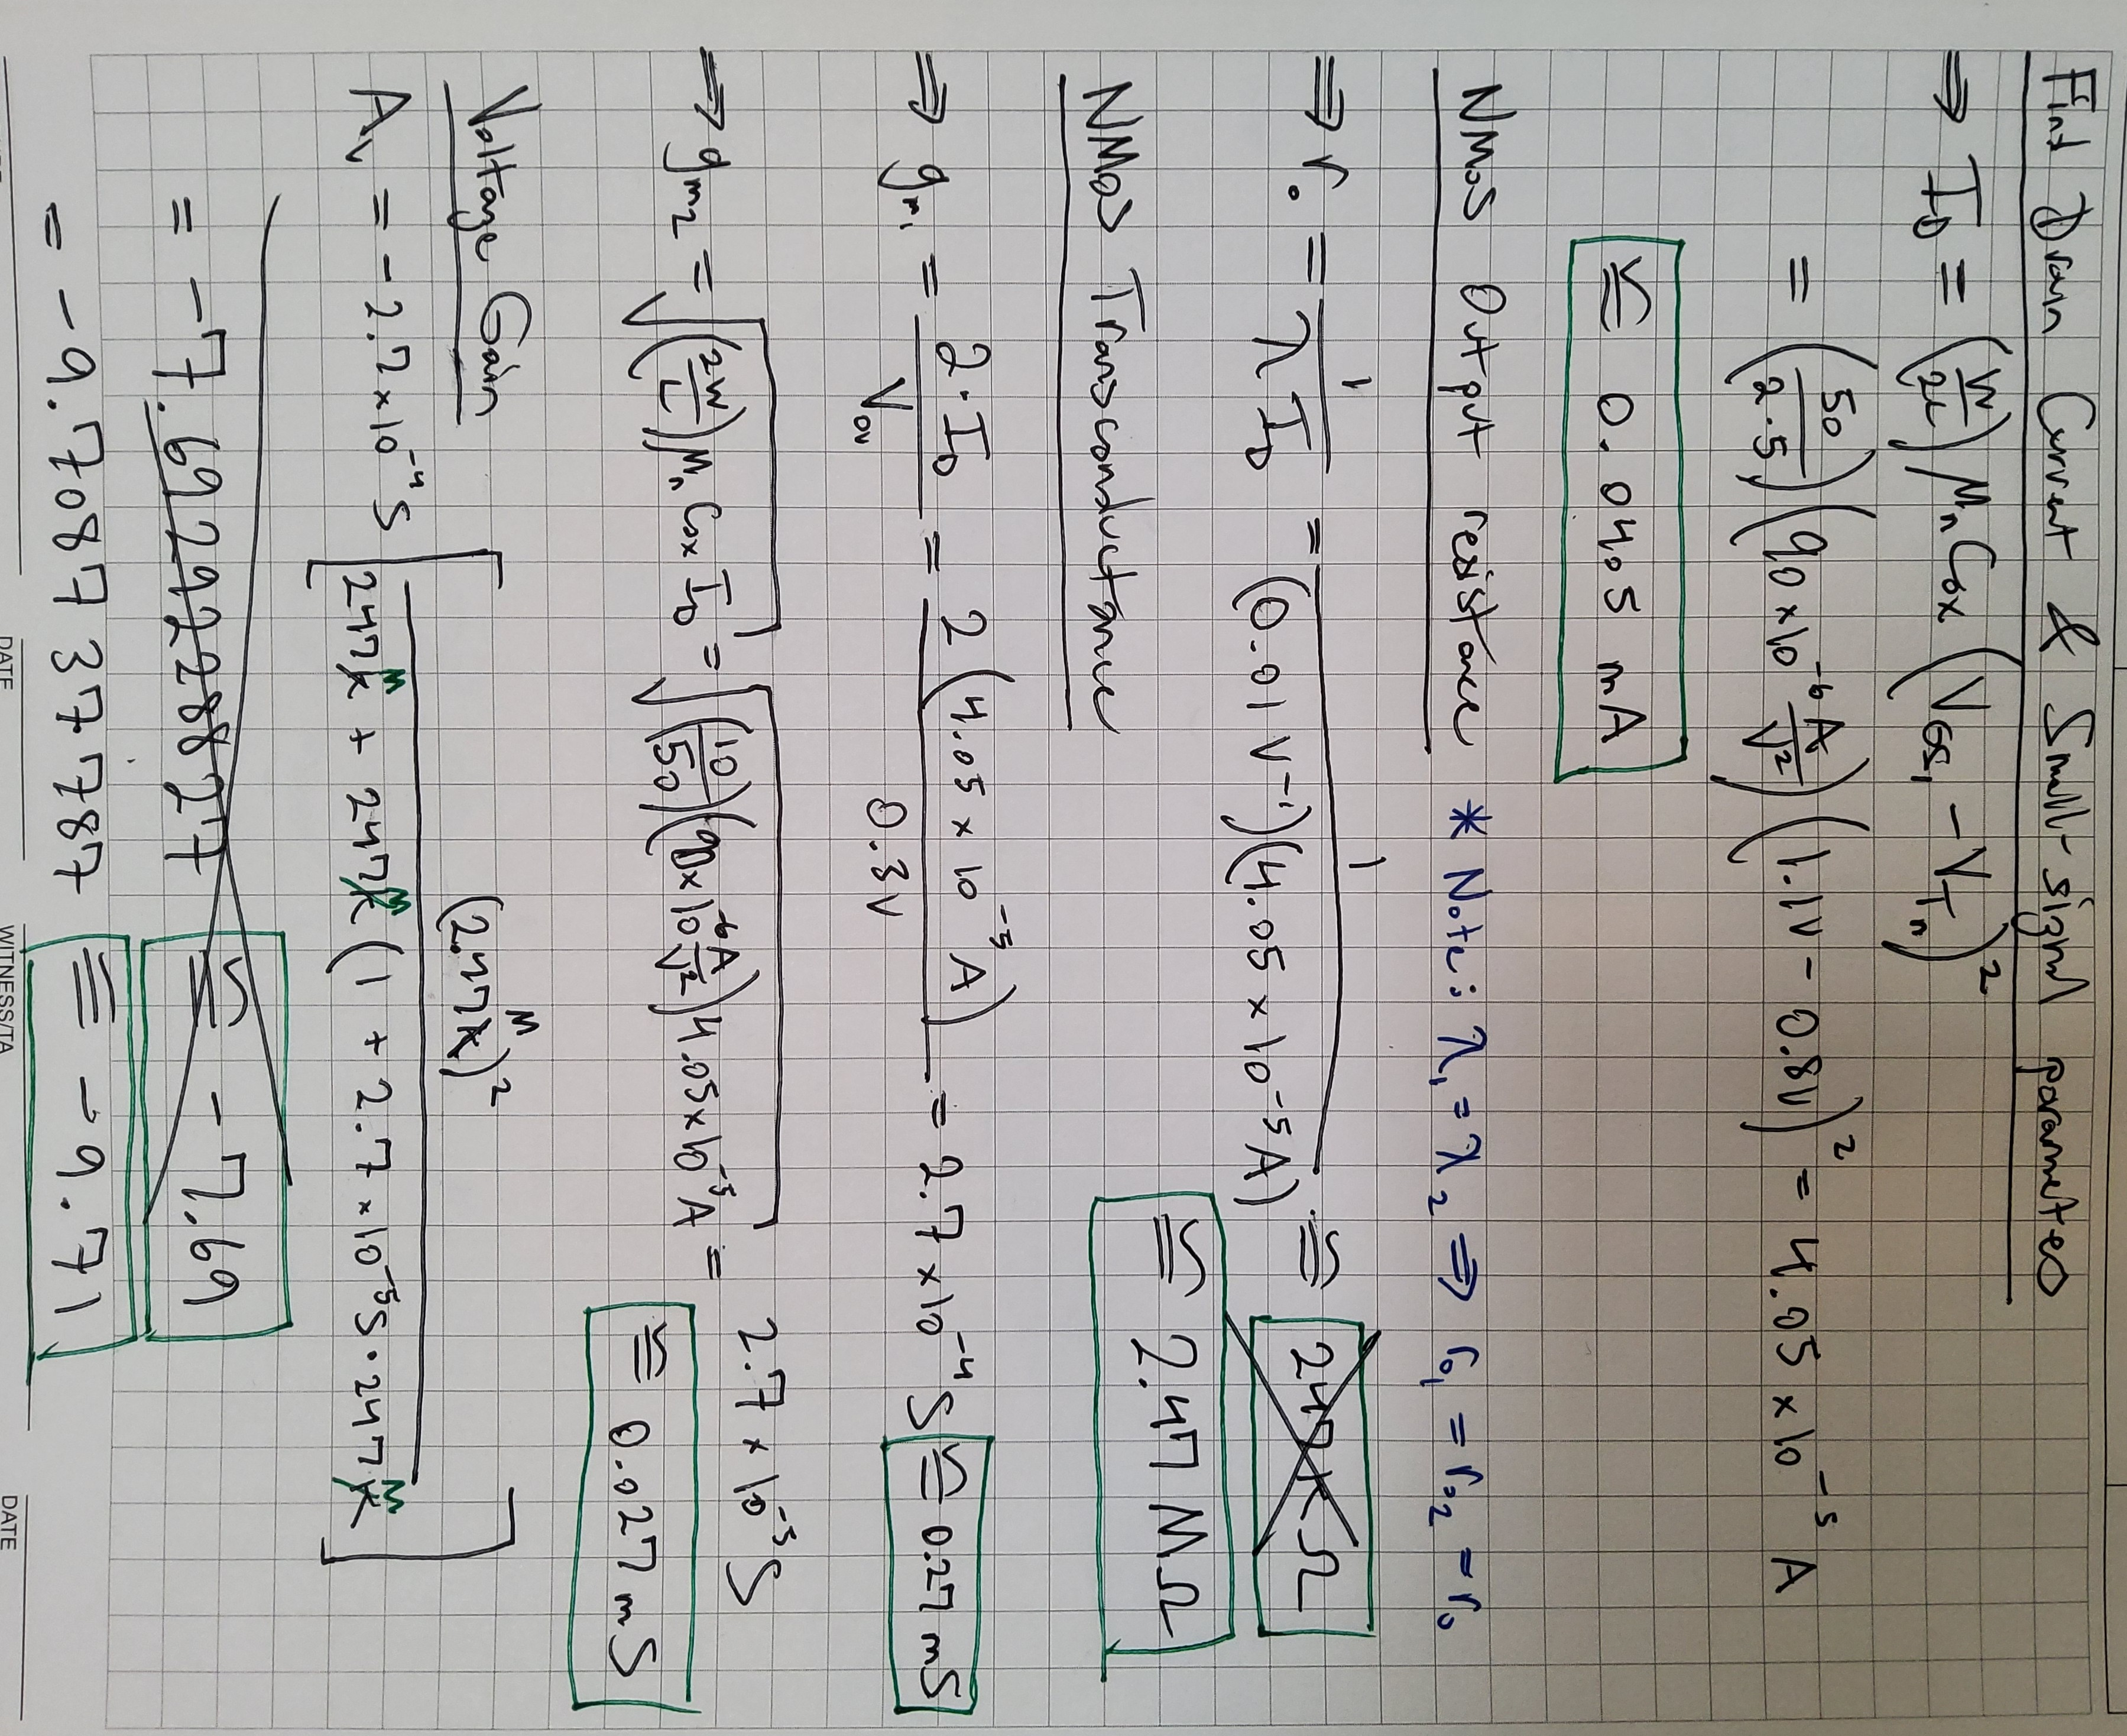
\includegraphics[scale=0.175, angle=90, center]{p1_2.jpg}\\
\newpage
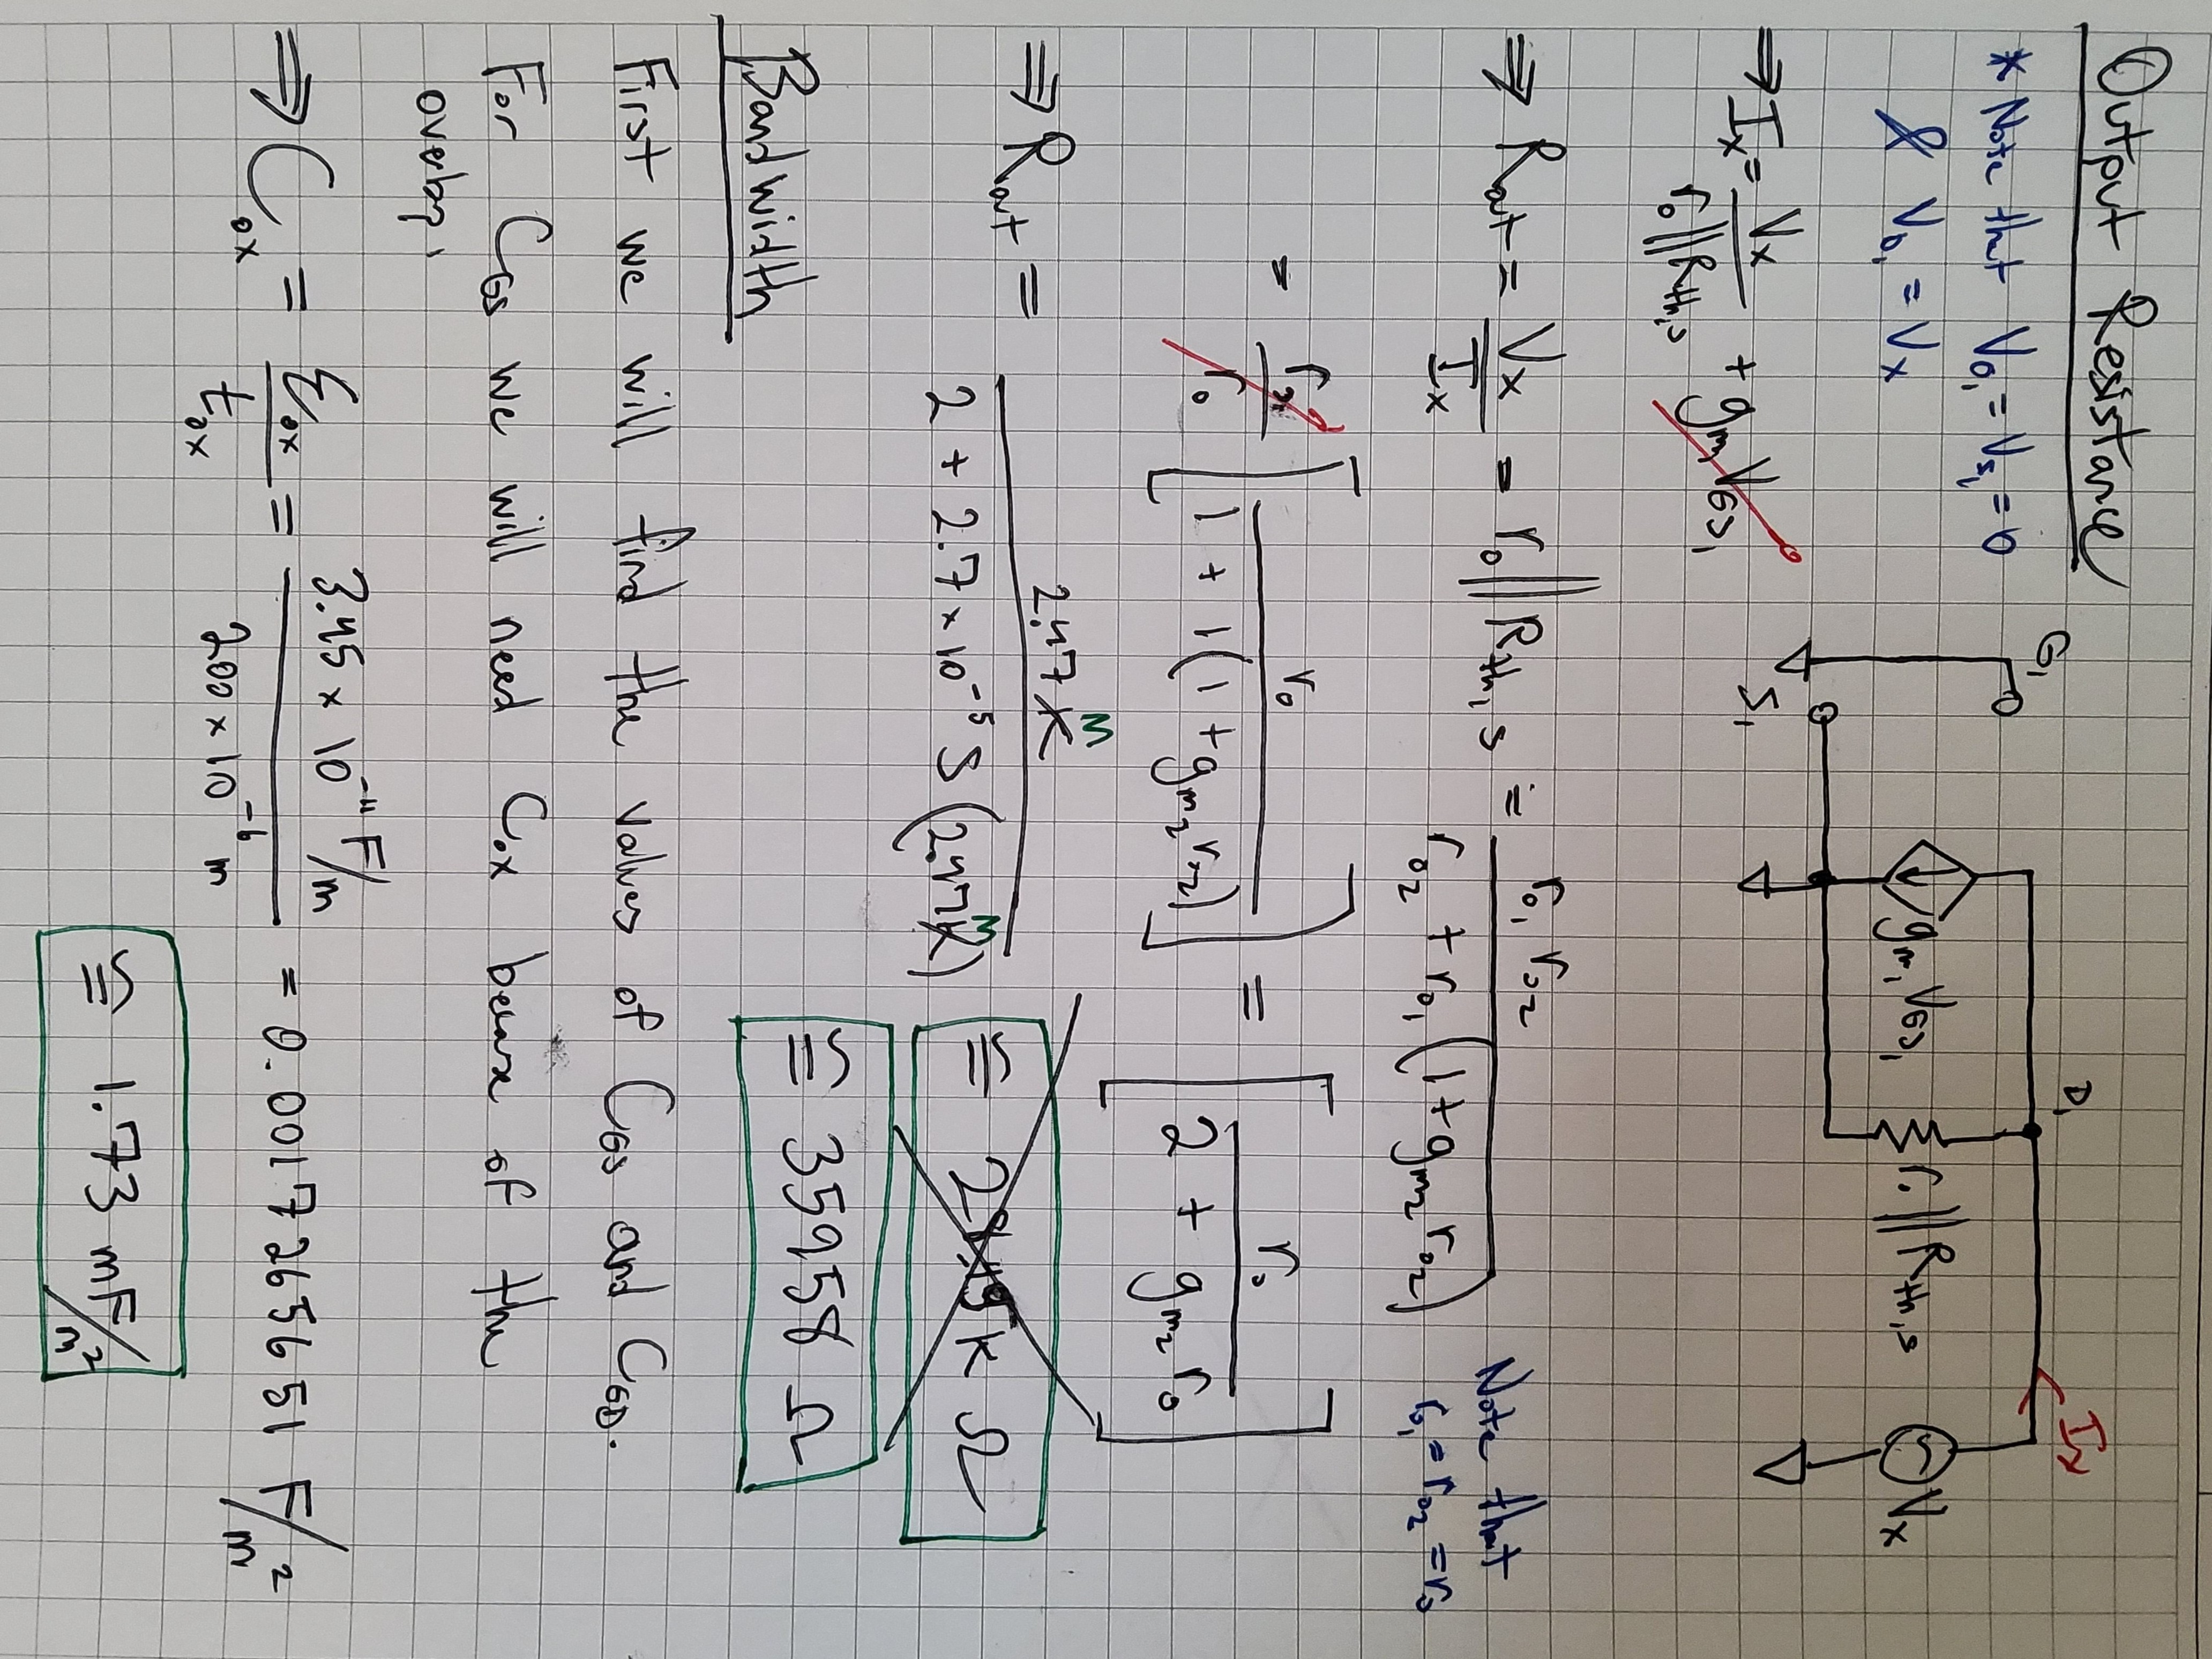
\includegraphics[scale=0.15, angle=90, center]{p1_3.jpg}\\
\newpage
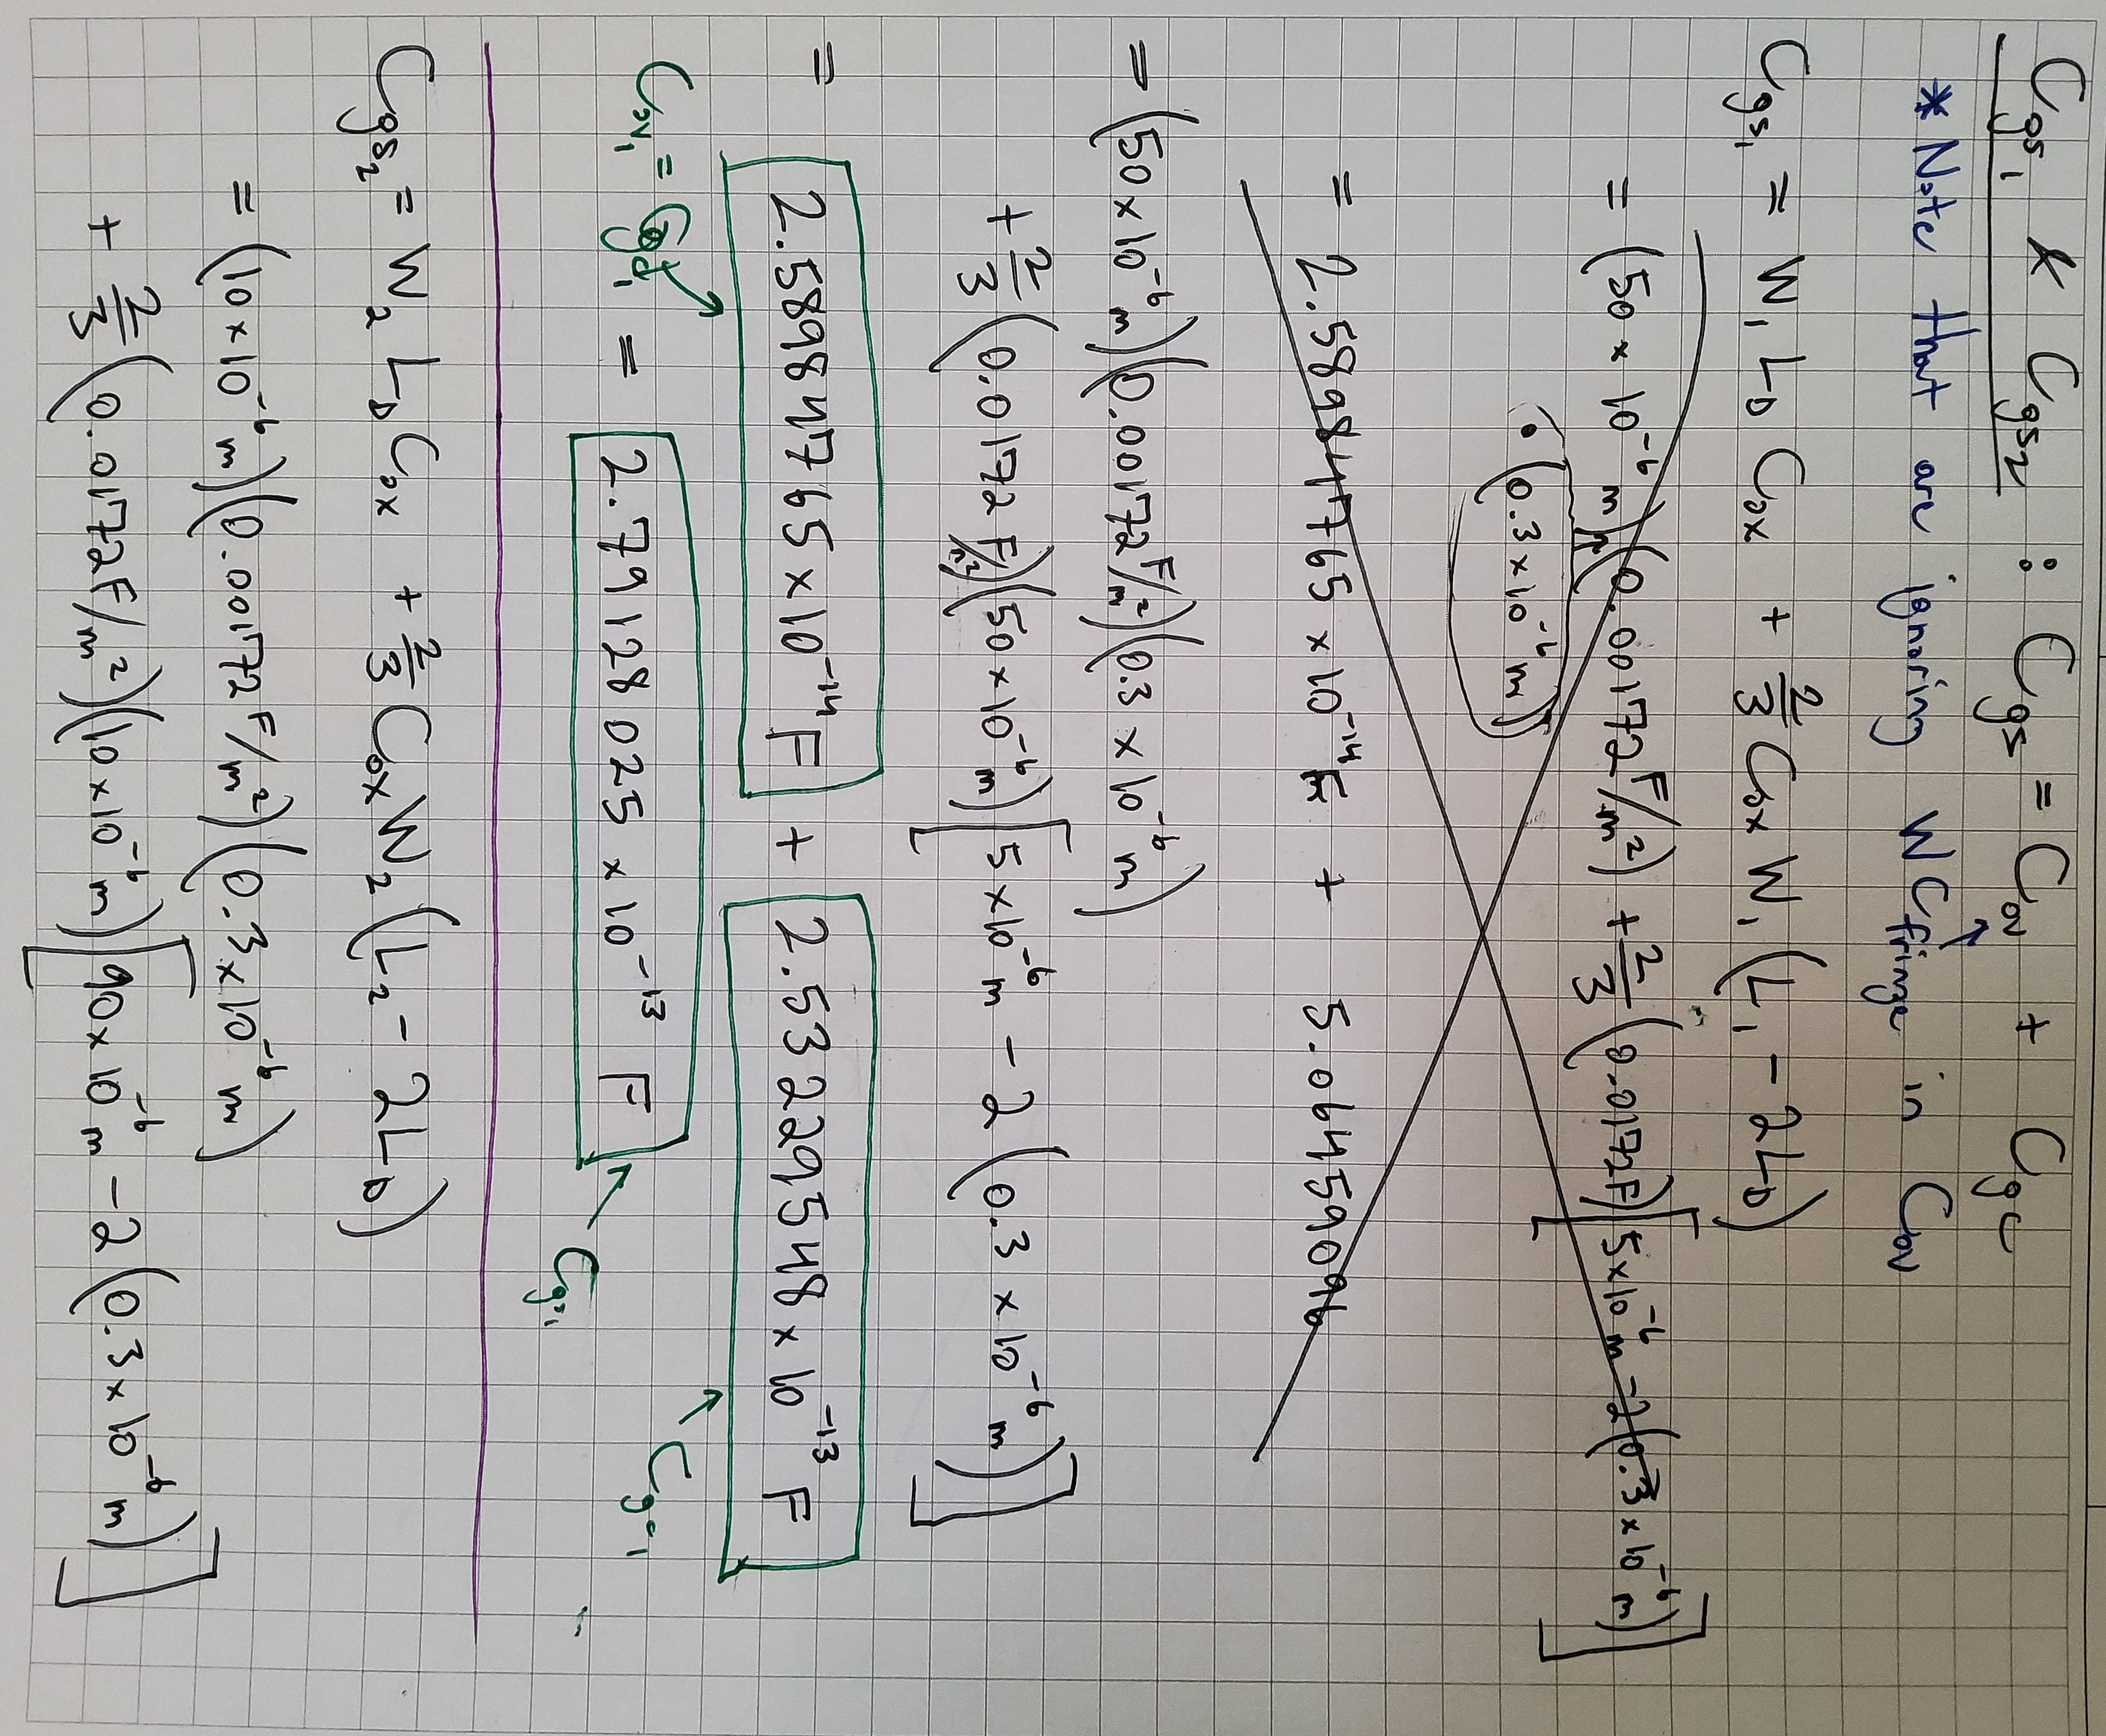
\includegraphics[scale=0.165, angle=90, center]{p1_4.jpg}\\
\newpage
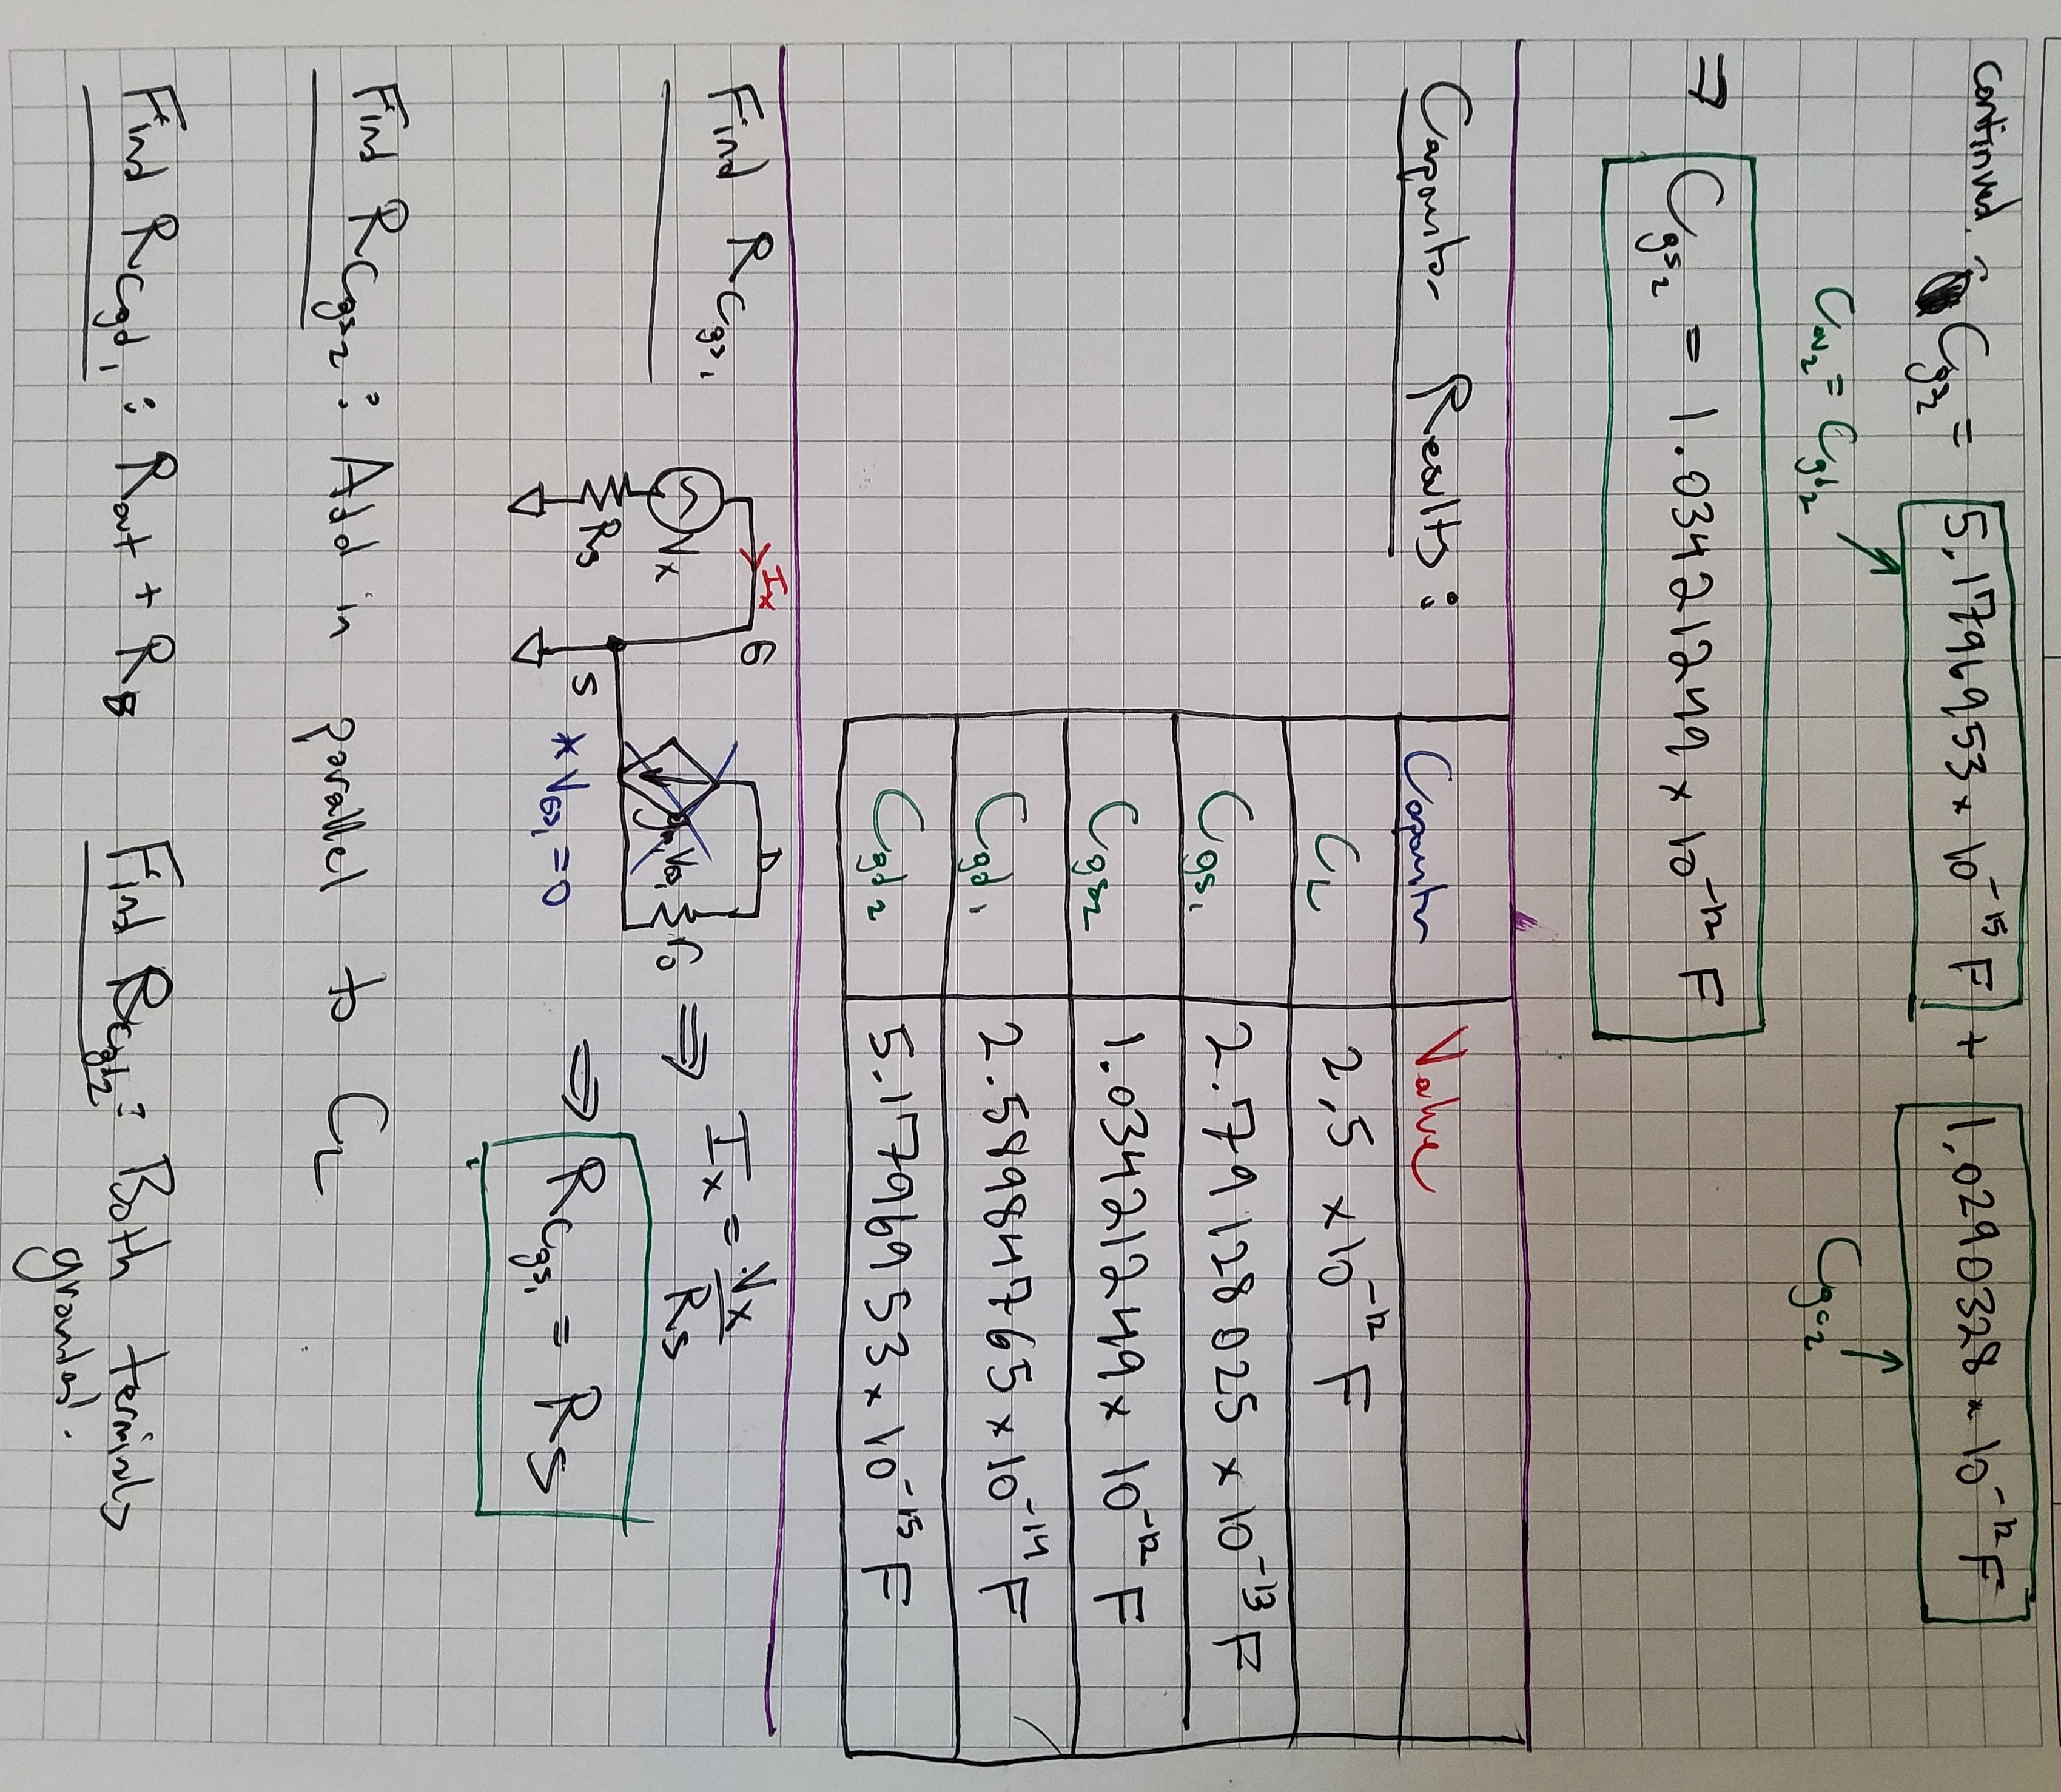
\includegraphics[scale=0.165, angle=90, center]{p1_5.jpg}\\
\newpage
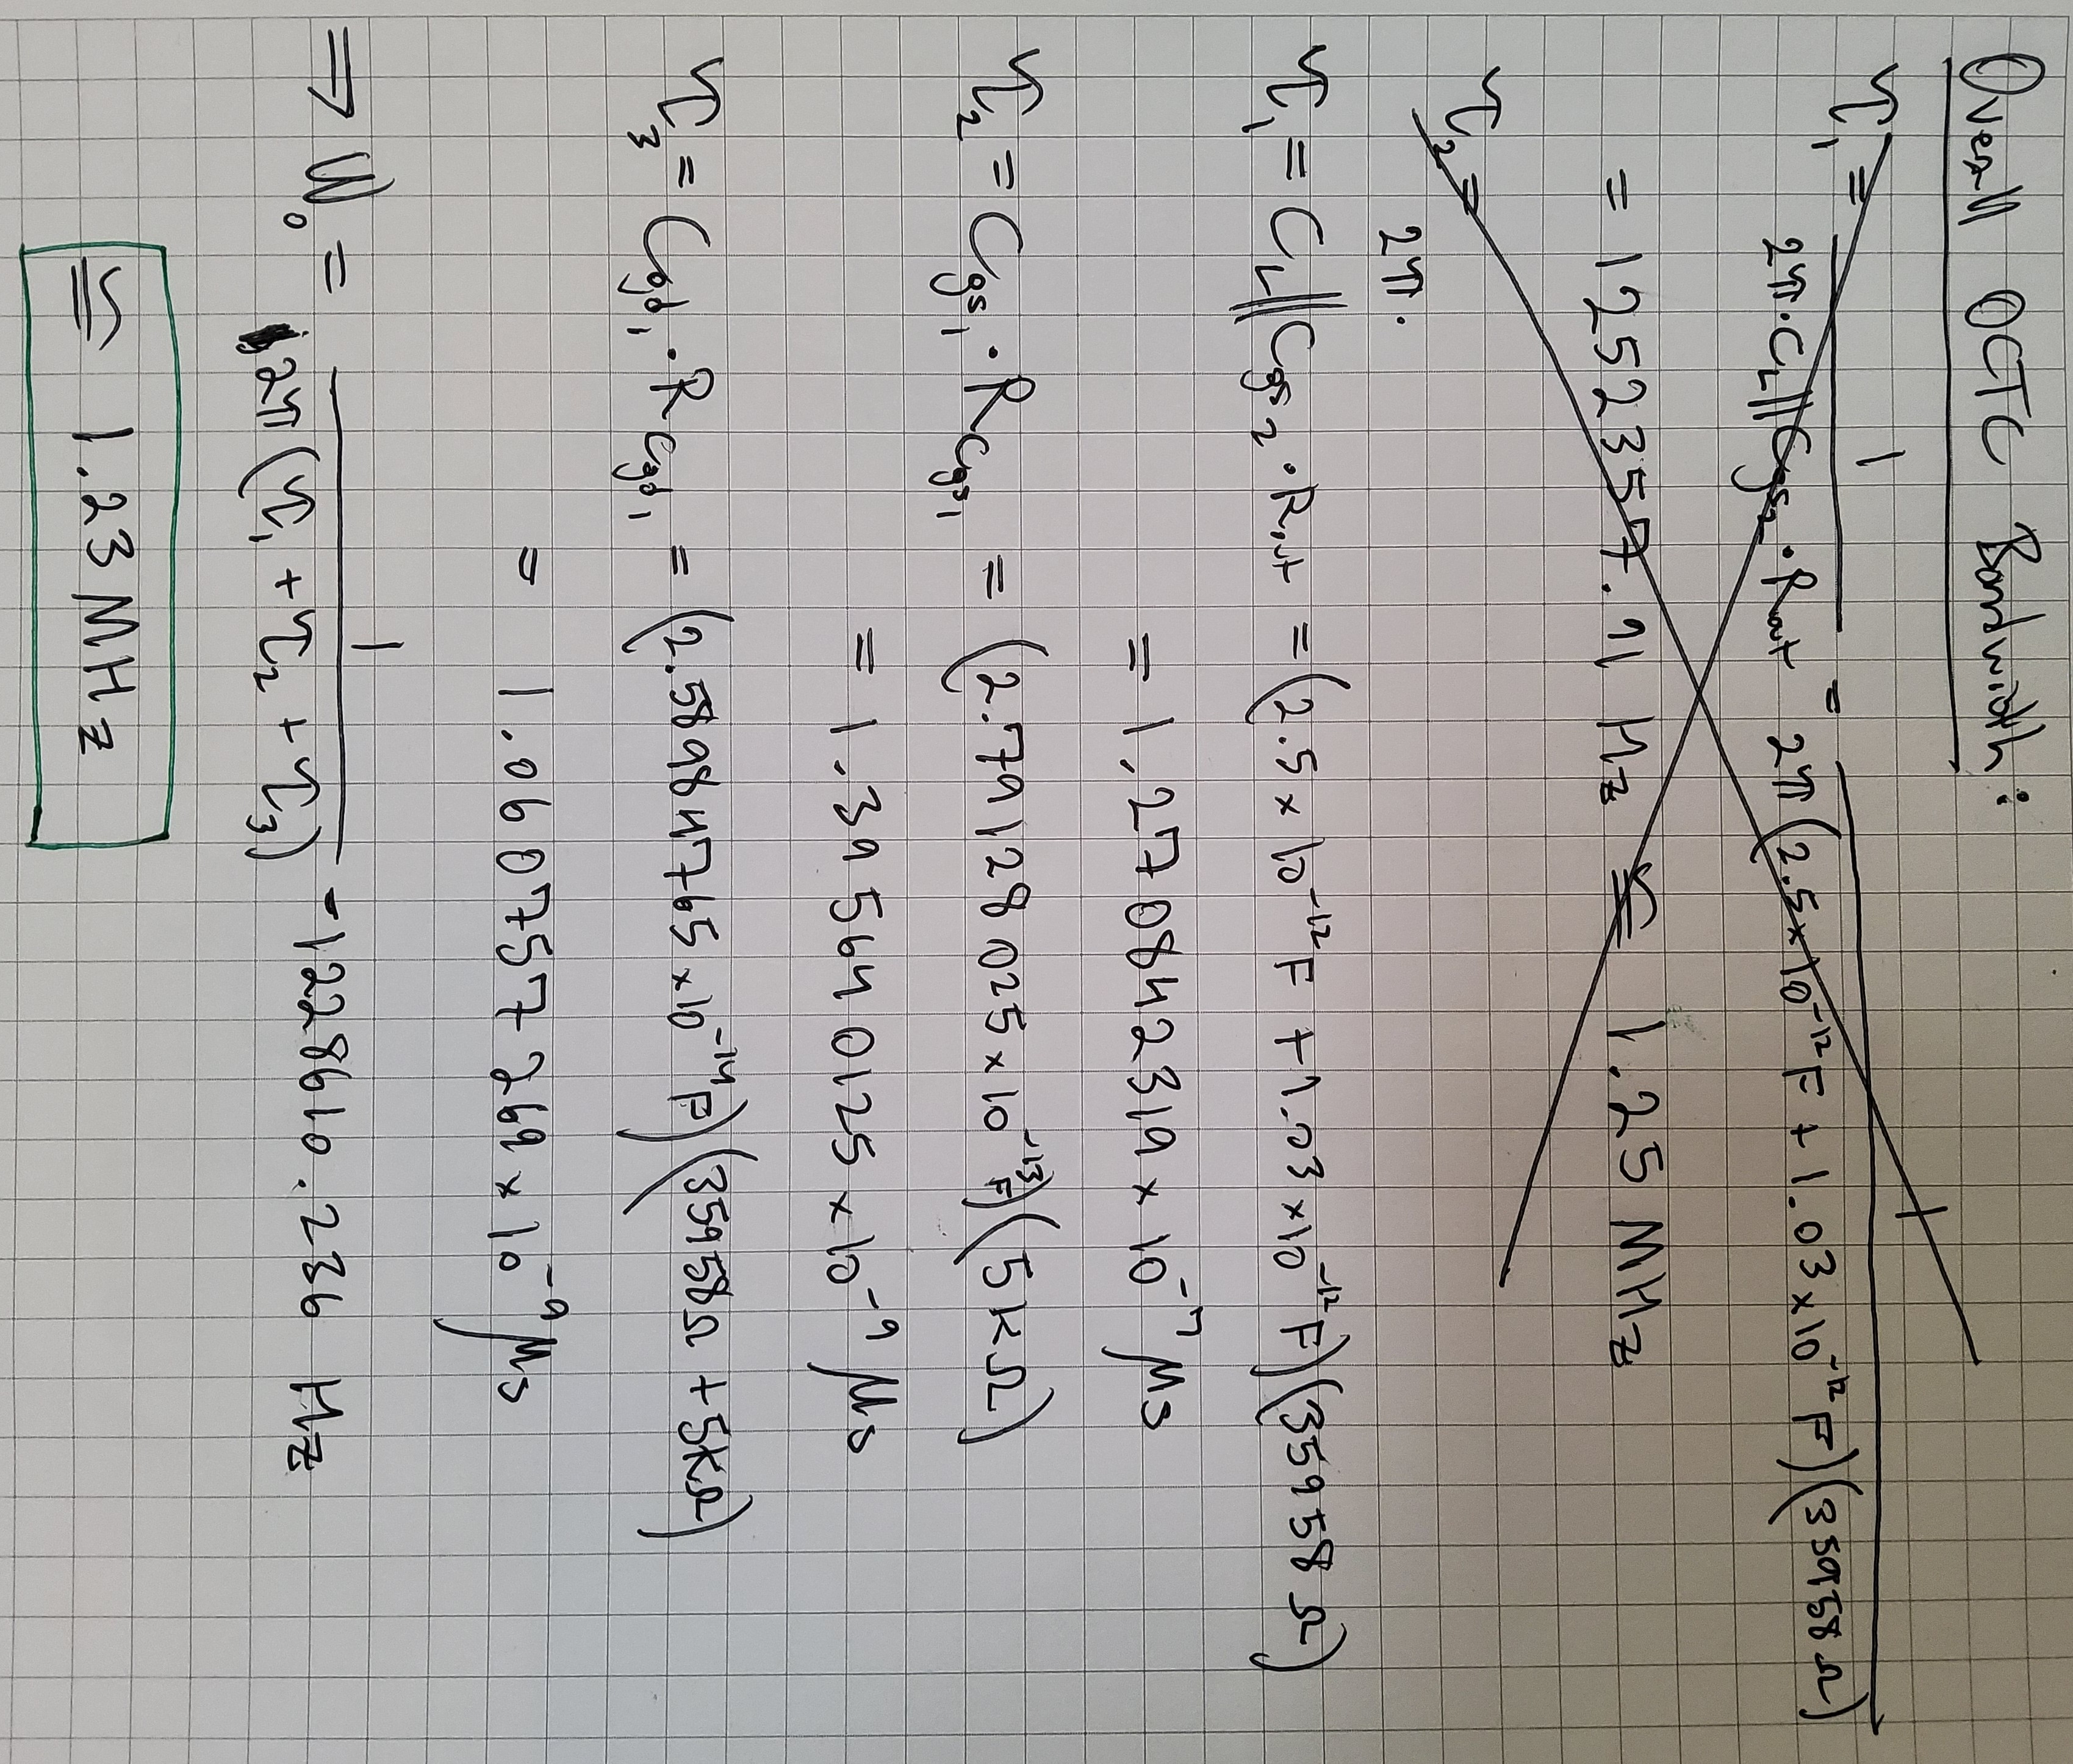
\includegraphics[scale=0.165, angle=90, center]{p1_6.jpg}\\
\newpage
%%%%%%%%%%%%%%%%%%%%%%%%%%%%%%%%%%%%%%%%
%               SIMULATION             %
%%%%%%%%%%%%%%%%%%%%%%%%%%%%%%%%%%%%%%%%
\subsubsection{Simulation}
Below is the internal schematic of the amplifier used for simulation:\\[0.1cm]
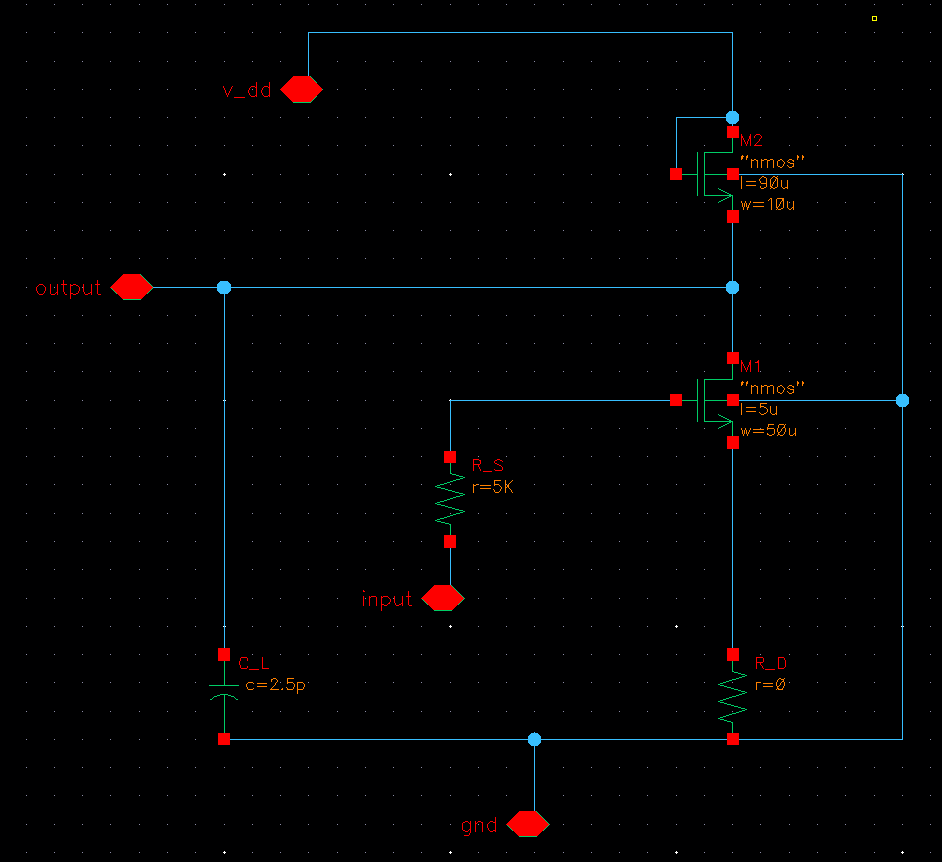
\includegraphics[scale=0.4, center]{a_internal.png}\\
Below is the symbol I created, and the testbench:\\[0.1cm]
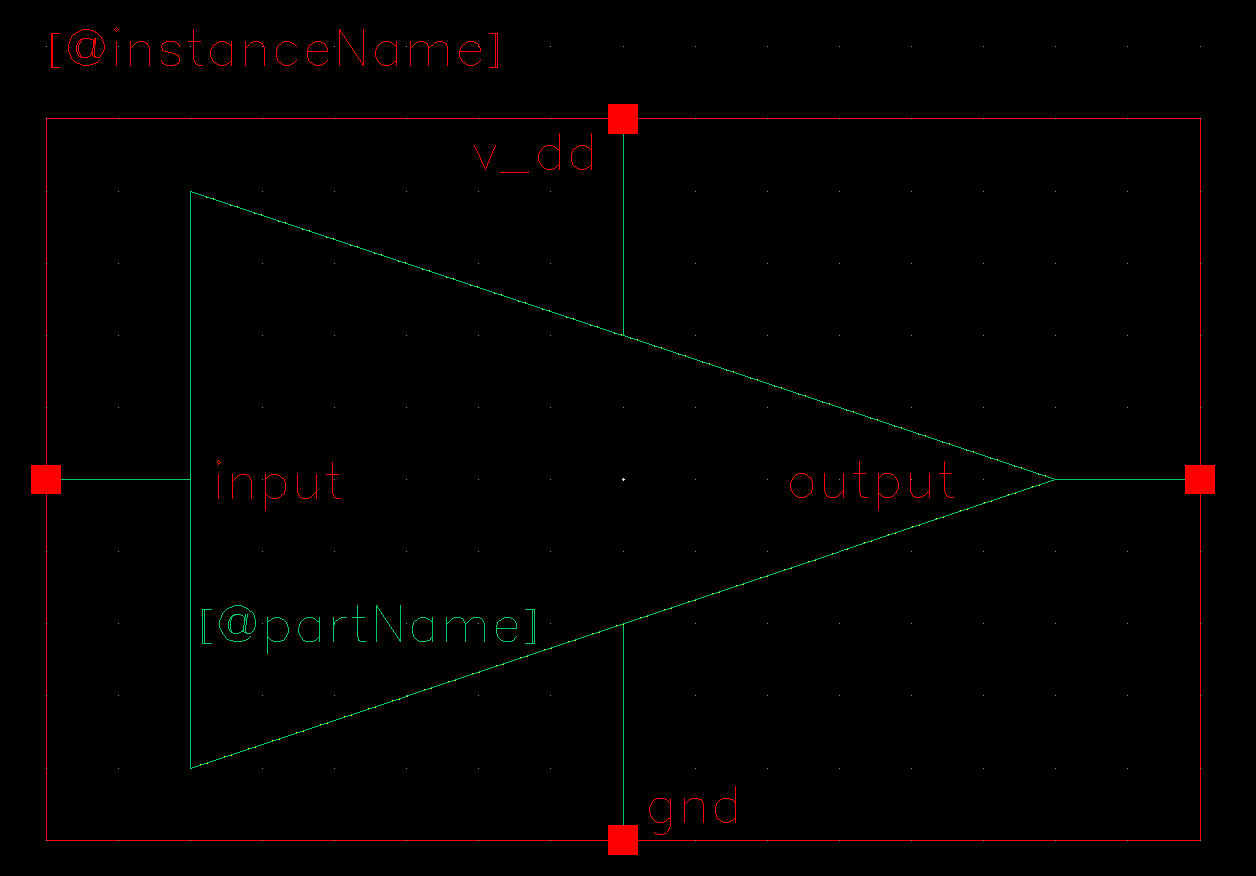
\includegraphics[scale=0.15, center]{a_symbol.png}
\quad
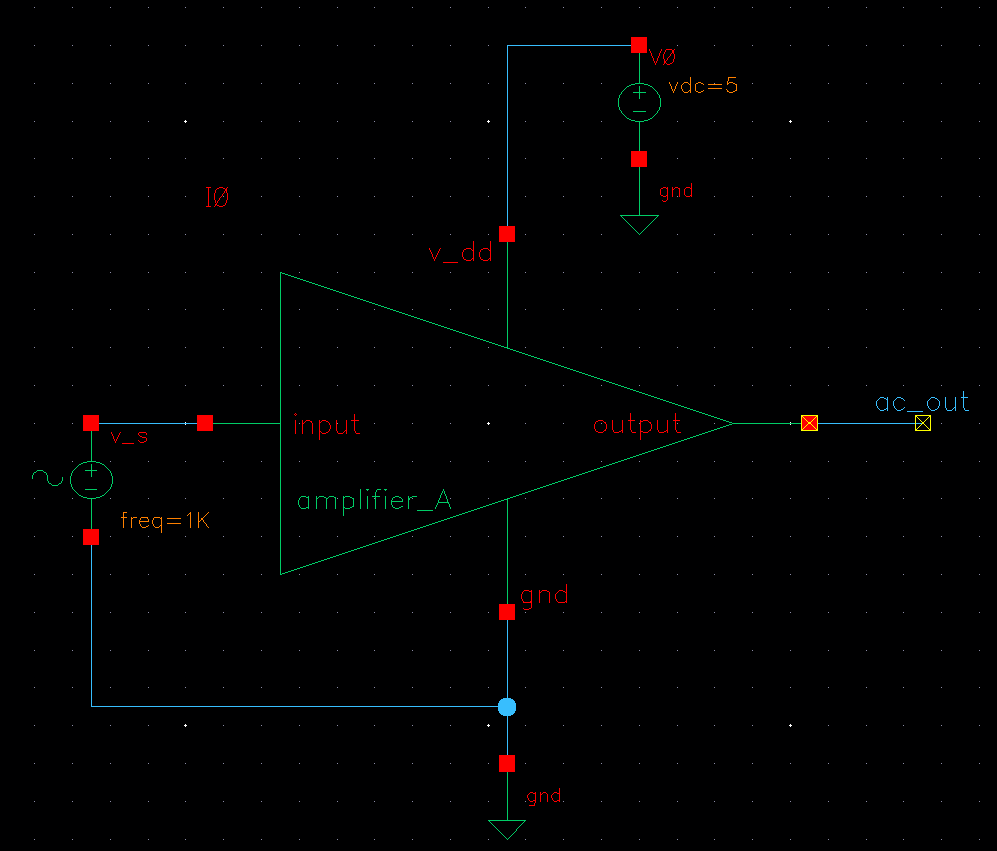
\includegraphics[scale=0.3, center]{a_tb.png}
\newpage
\begin{enumerate}
    \item
    {
    \textbf{\underline{Voltage Gain and Bandwidth}}\\[0.25cm]
    Below is the plot of the magnitude of the gain for the amplifier:\\[0.1cm]
    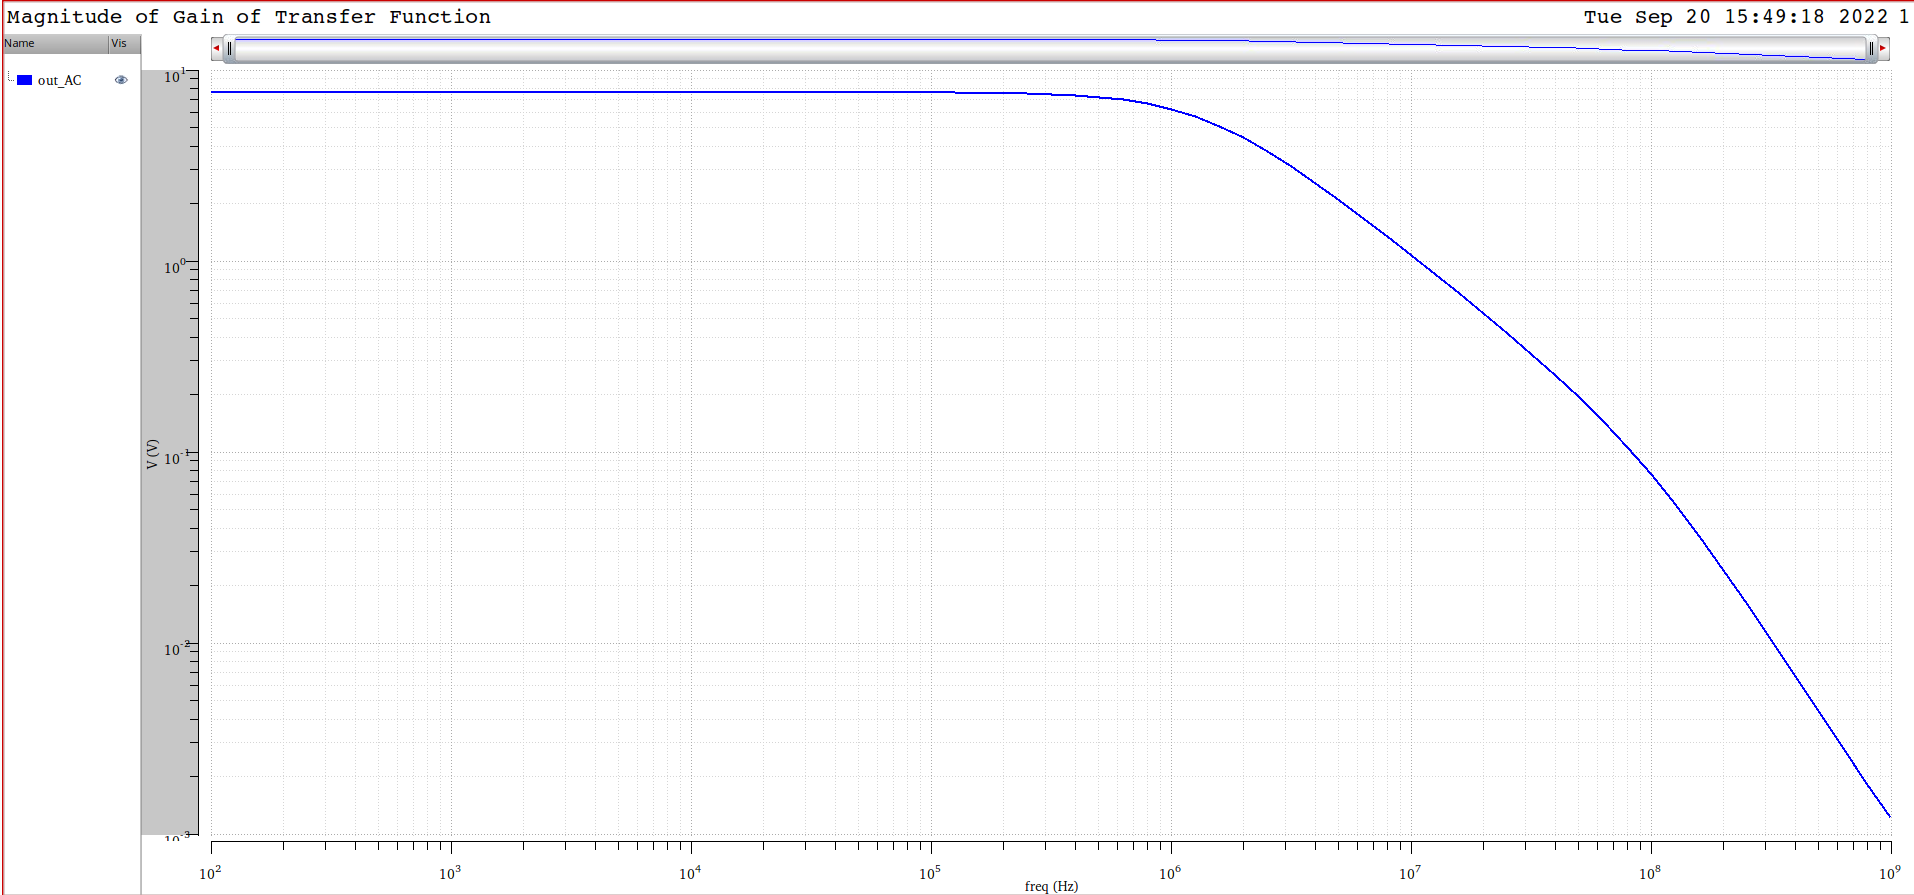
\includegraphics[scale=0.35, center]{a_plot.png}\\[1cm]
    Below are the simulated values for the voltage gain and bandwidth:\\[0.1cm]
    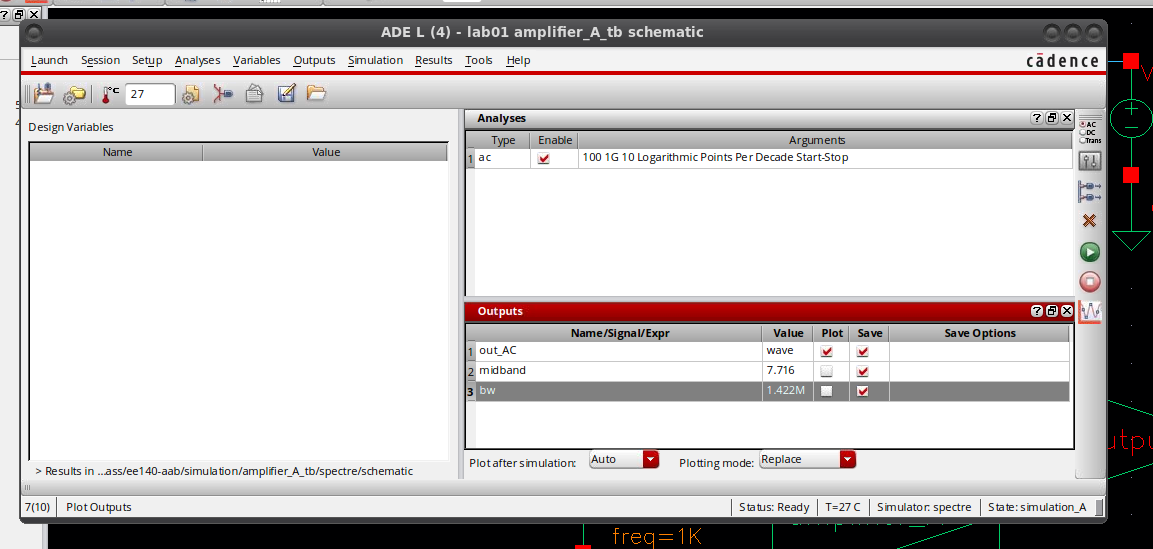
\includegraphics[scale=0.55, center]{a_gbw.png}\\
    }
    \newpage
    \item
    {
    \textbf{\underline{Output Resistance}}\\[0.25cm]
    Below is the simulated value of the output resistance using transient analysis:\\[0.1cm]
    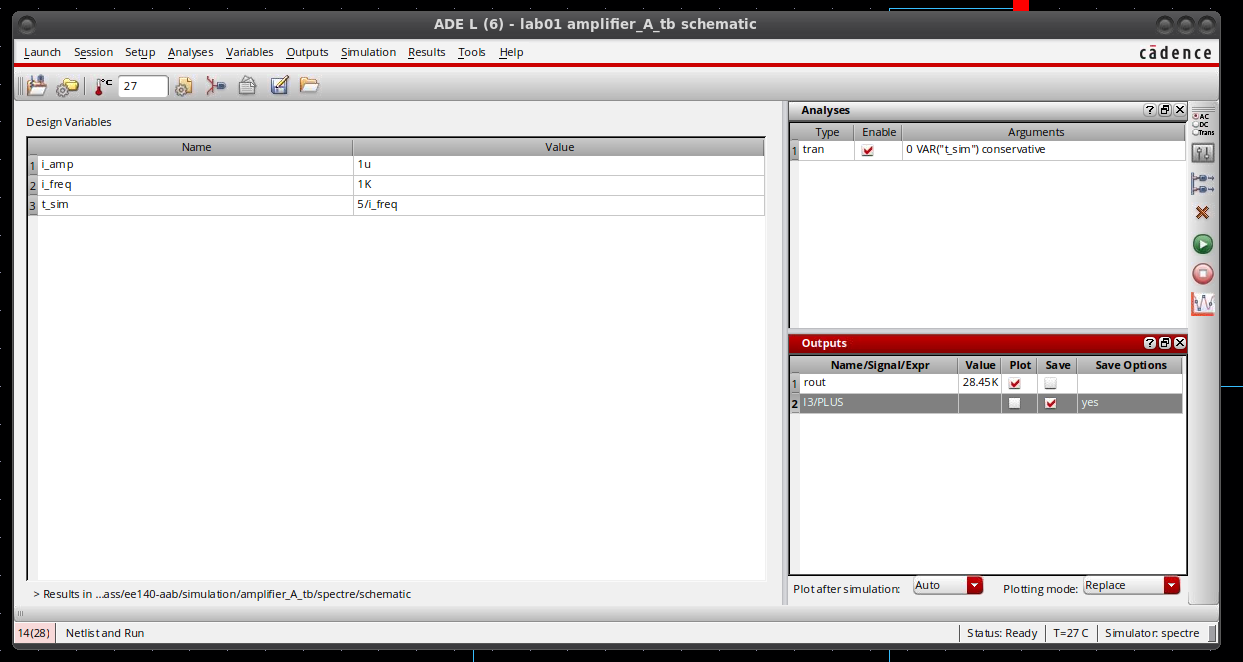
\includegraphics[scale=0.5, center]{a_rout.png}\\[0.5cm]
    }
    \item
    {
    \textbf{\underline{Output Voltage Swing}}\\[0.25cm]
    Below is the simulated value of the output voltage swing using the $1\,dB$ compression point:\\[0.1cm]
    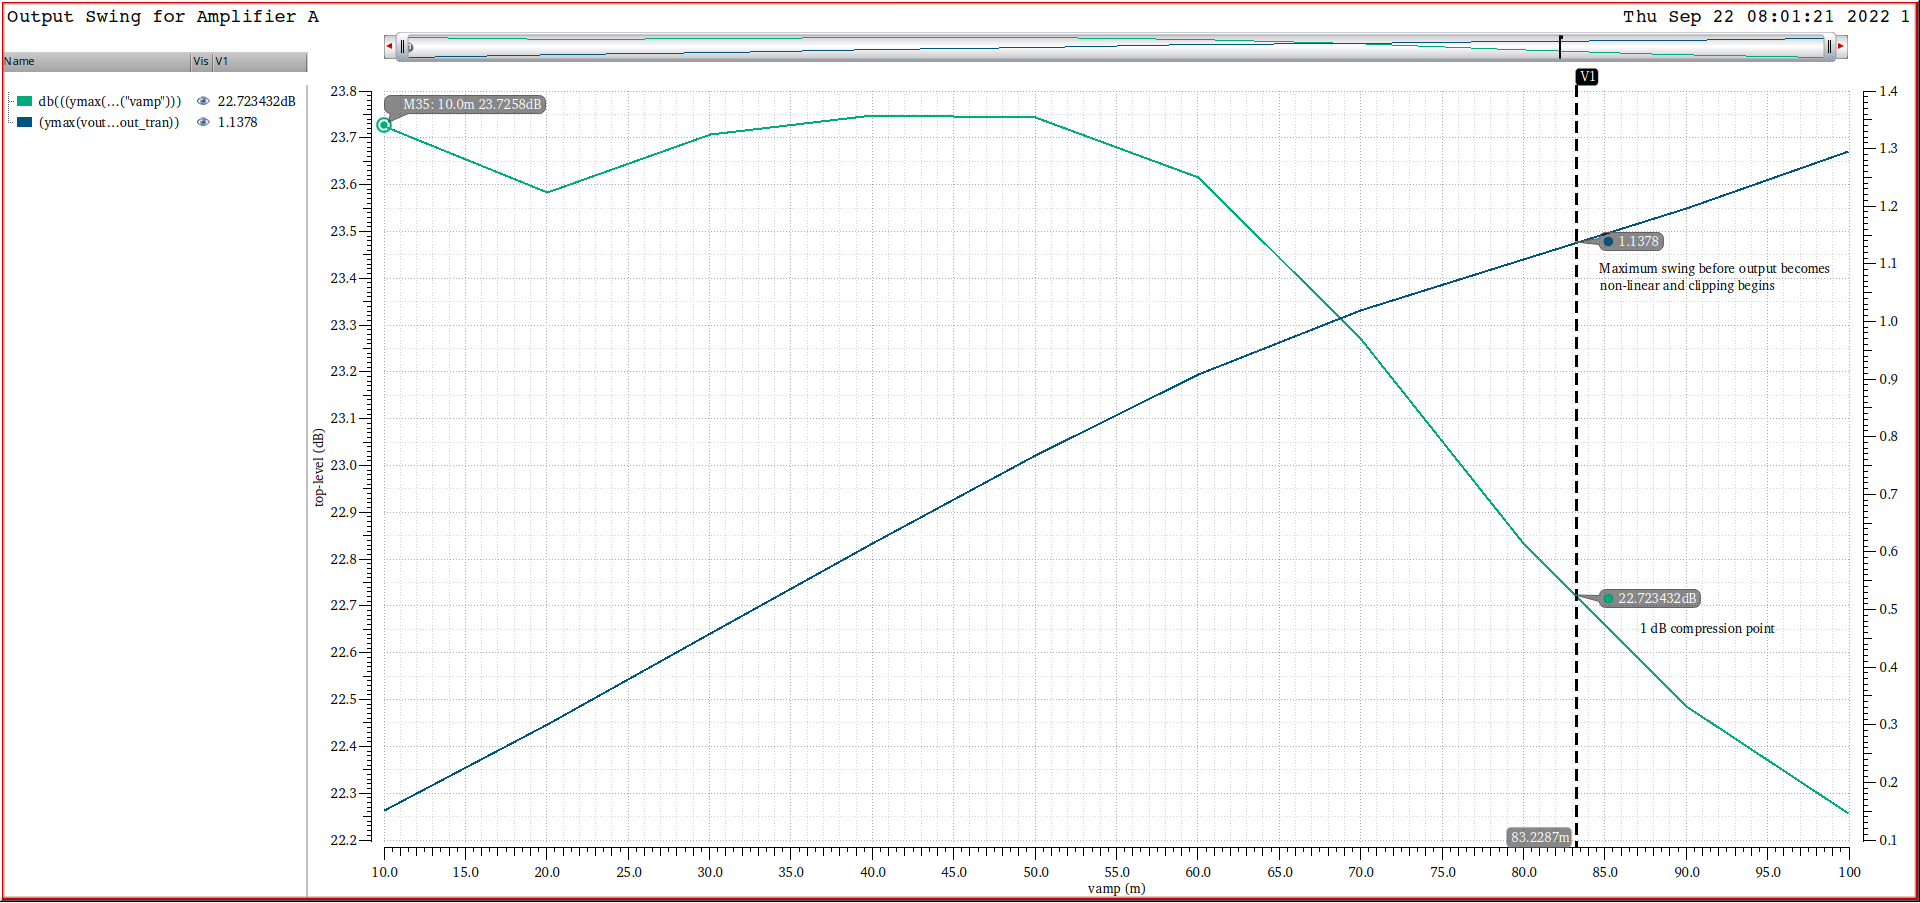
\includegraphics[scale=0.35, center]{a_swing.png}\\[0.5cm]
    }
\end{enumerate}
\newpage
%%%%%%%%%%%%%%%%%%%%%%%%%%%%%%%%%%%%%%%%
%                 RESULTS              %
%%%%%%%%%%%%%%%%%%%%%%%%%%%%%%%%%%%%%%%%
\subsubsection{Results}
Below is a table of results for both the hand calculations and simulated values:\\[0.25cm]
\begin{table}[H]
\centering
\setlength{\tabcolsep}{20pt}
\renewcommand{\arraystretch}{1.5}
\begin{tabular}{|l|c|c|}
    \hline
    \textbf{\textit{Parameter}} & \textbf{\textit{Hand Calculated Value}} & \textbf{\textit{Simulated Value}}\\
    \hline
    $\left|\text{\textit{Voltage Gain}}\right|$ & $9.71\,V/V$ & $7.716\,V/V$\\
    \hline
    \textit{Bandwidth} & $1.23\,MHz$ & $1.422\,MHz$\\
    \hline
    \textit{Output Resistance} & $35.96\,k\Omega$ & $28.45\,k\Omega$ \\
    \hline
    \textit{Voltage Swing} & X & $1.1378\,V$\\
    \hline
\end{tabular}
\caption{Results for amplifier in \textit{Task A}.}
\end{table}
\noindent
\underline{\textbf{\textit{Summary of Results}}}\\[0.25cm]
All of the hand calculations do not quite match the simulated values.  The discrepancy in the gain is almost certainly due to neglecting the body effect.  The body effect will increase the threshold voltage, which in turn reduces the overdrive voltage.  A smaller overdrive voltage results in a smaller saturation drain current, and thus less voltage gain.

The discrepancy in the output resistance is due to neglecting the channel length modulation.  When calculating the saturation drain current CLM was ignored, which means that our hand-calculated $I_D$ will be slightly less than it should be.  Since we calculated $r_o$ with $1/\lambda I_D$, its value will be larger than it actually is.  Because $r_o$ is the dominant term in the numerator of the output resistance hand calculation, the output resistance will be larger than its simulated value, which is what we see. 

Ignoring the CLM also propagates into the discrepancy of the bandwidth.  Although we were thorough in calculating the OCTC BW, the dominant pole is calculated with the output resistance.  Because we can already see that there is an error in that hand calculation, it spills over into our hand calculation for the BW.
\newpage
%%%%%%%%%%%%%%%%%%%%%%%%%%%%%%%%%%%%%%%%%%%%%%%%%%%%%%
%                       TASK B                       %
%%%%%%%%%%%%%%%%%%%%%%%%%%%%%%%%%%%%%%%%%%%%%%%%%%%%%%
\subsection{Task B}
\textbf{\emph{Given: }}\\[0.25cm]
\noindent
In this part we add some degeneracy into the circuit by changing the value of resistor $R_D$. You can assume that:\\[0.25cm]
\begin{table}[H]
\centering
\setlength{\tabcolsep}{20pt}
\renewcommand{\arraystretch}{1.5}
\begin{tabular}{|l|c|}
    \hline
    $V_{B1}$ & $1.2\,V$\\
    \hline
    $R_D$ & $2.5\,k\,\Omega$\\
    \hline
    $\frac{W}{L}_1$ & $10$\\
    \hline
    $\frac{W}{L}_2$ & $\frac{1}{9}$\\
    \hline
\end{tabular}
\caption{Modified amplifier parameters.
\label{tab:amp_param2}} 
\end{table}
\noindent
\textbf{\emph{Find: }}\\[0.25cm]\noindent
With the modified parameters, repeat the same process done in \textit{Task A}.\\[0.25cm]
\newpage\noindent
\textbf{\emph{Solution: }}
%%%%%%%%%%%%%%%%%%%%%%%%%%%%%%%%%%%%%%%%
%            HAND CALCULATIONS         %
%%%%%%%%%%%%%%%%%%%%%%%%%%%%%%%%%%%%%%%%
\subsubsection{Hand Calculations}

For the hand calculations we will again be ignoring the body effect and channel length modulation.  With the addition of the source degeneration due to the added resistor, the capacitance values will not change (and do not need to be recalculated), but the gain and resistances do.\\[0.25cm]
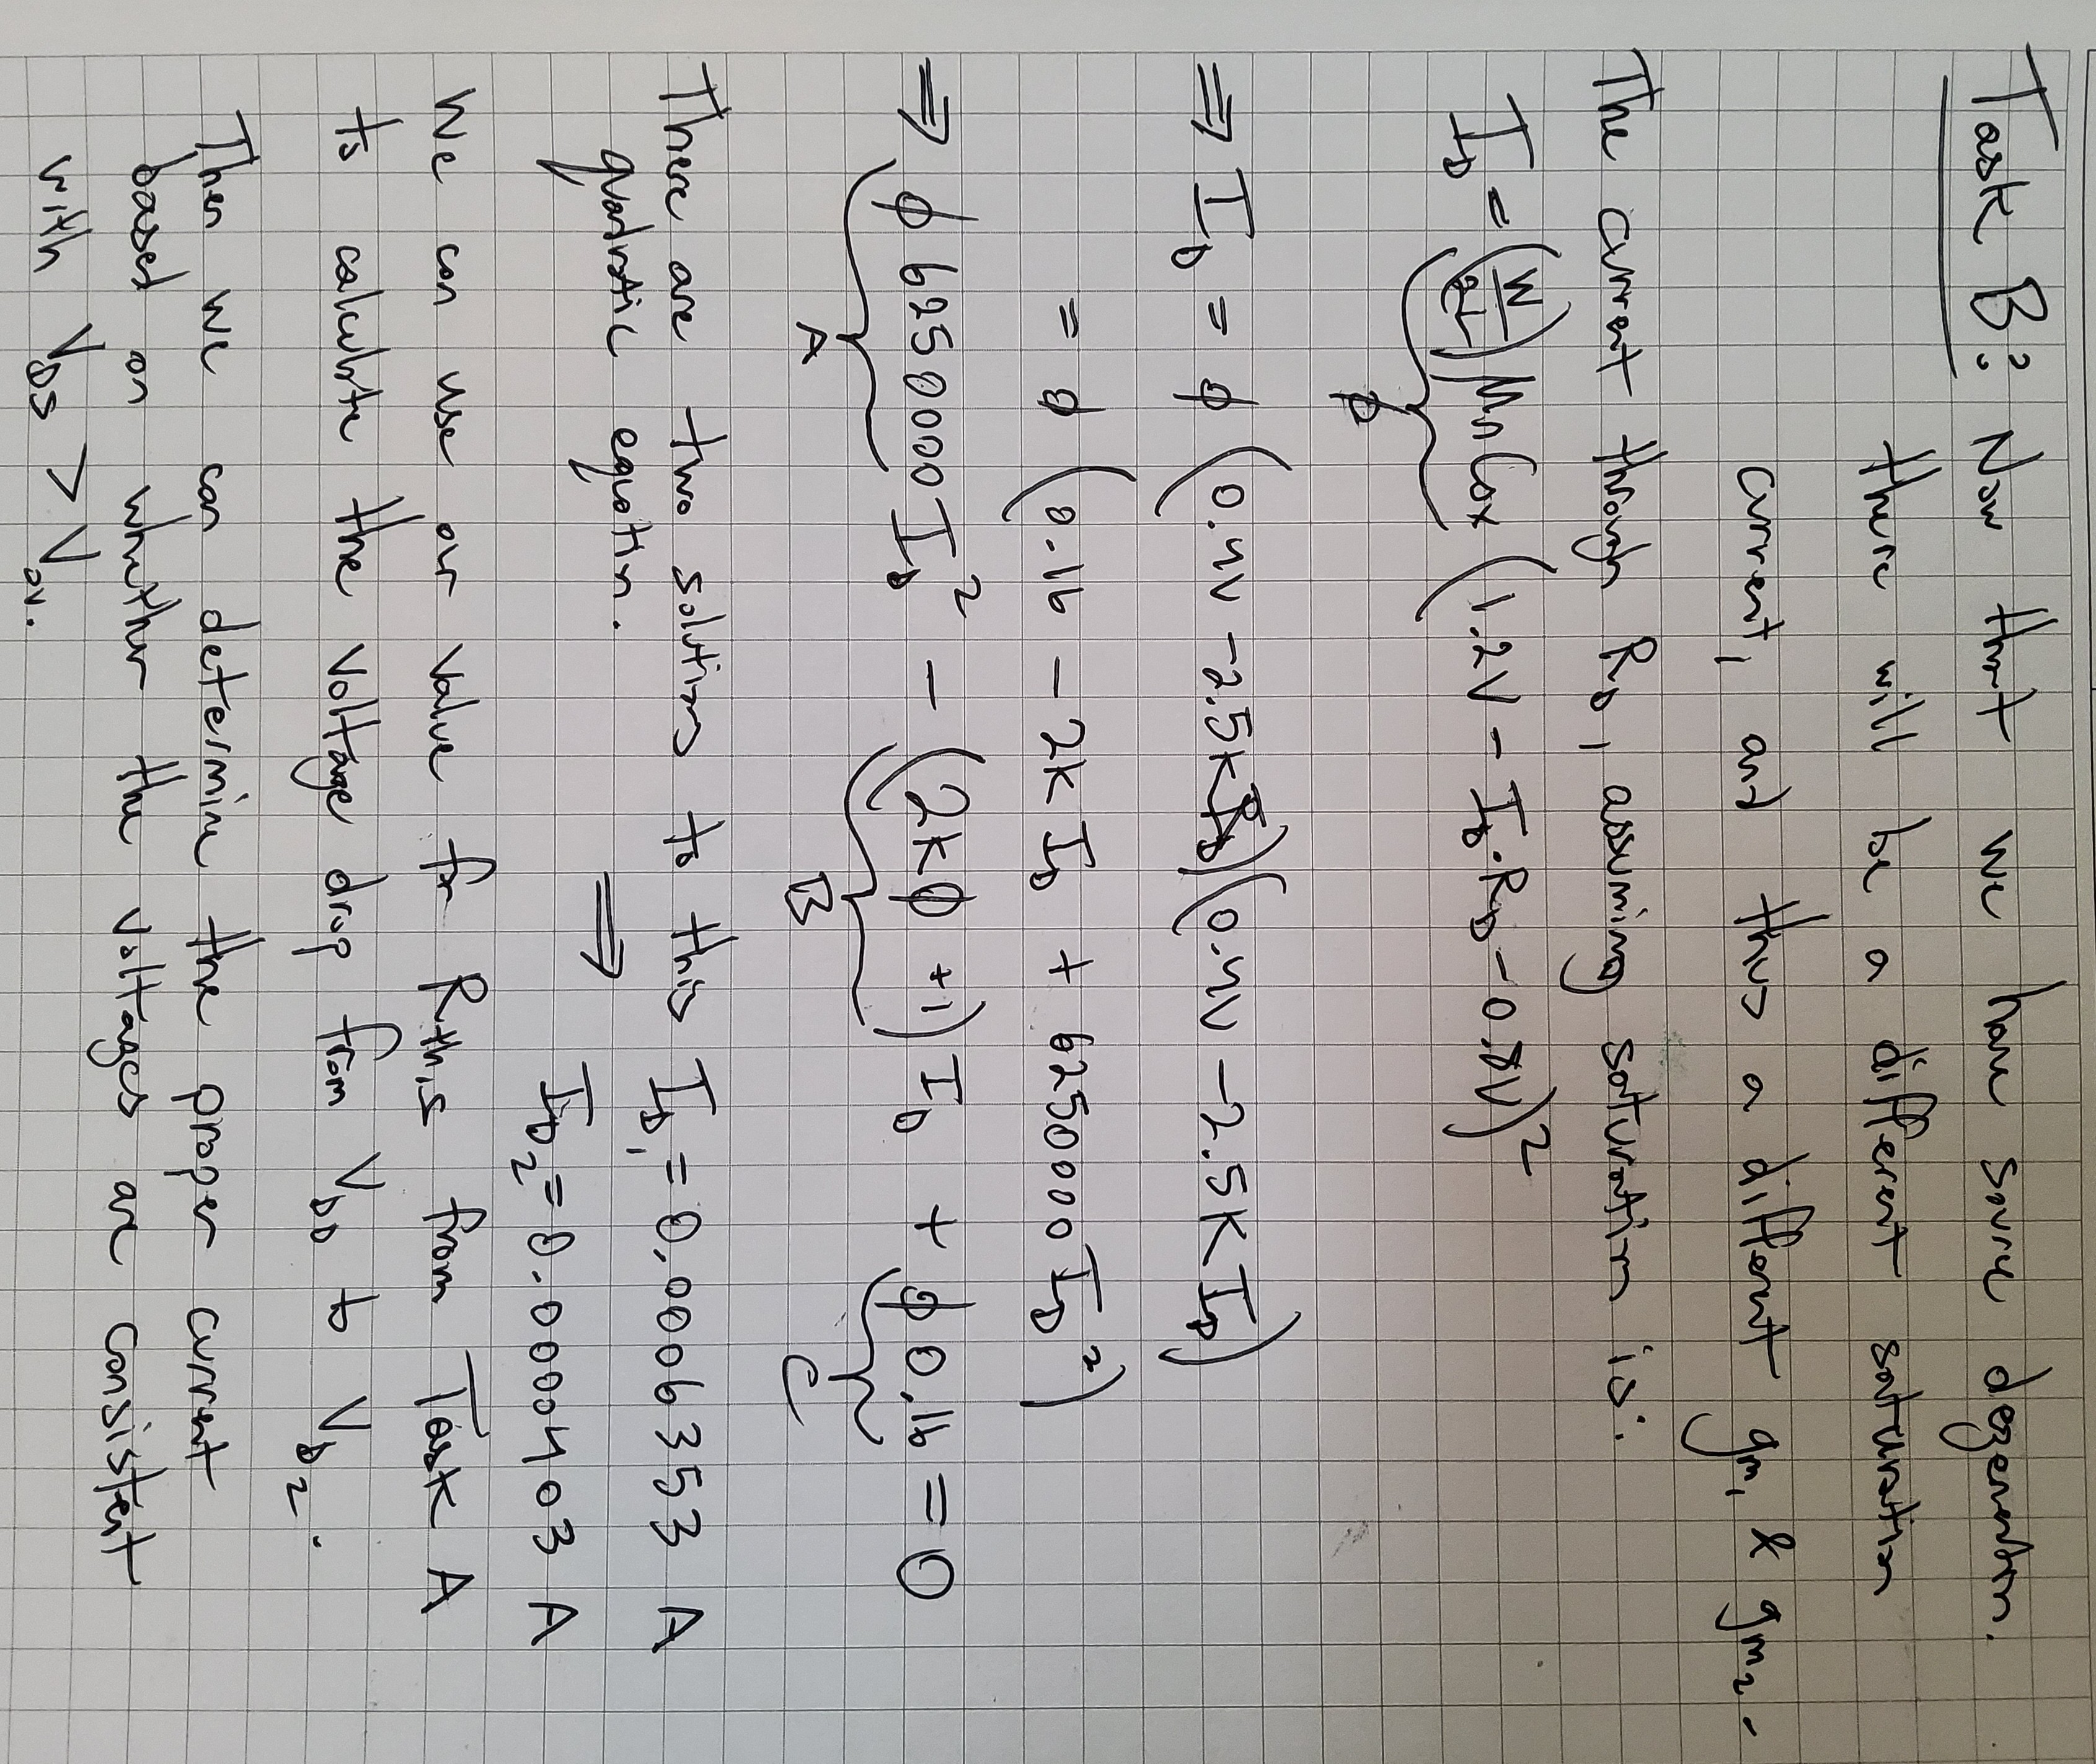
\includegraphics[scale=0.15, angle=90, center]{p1_7.jpg}\\
\newpage
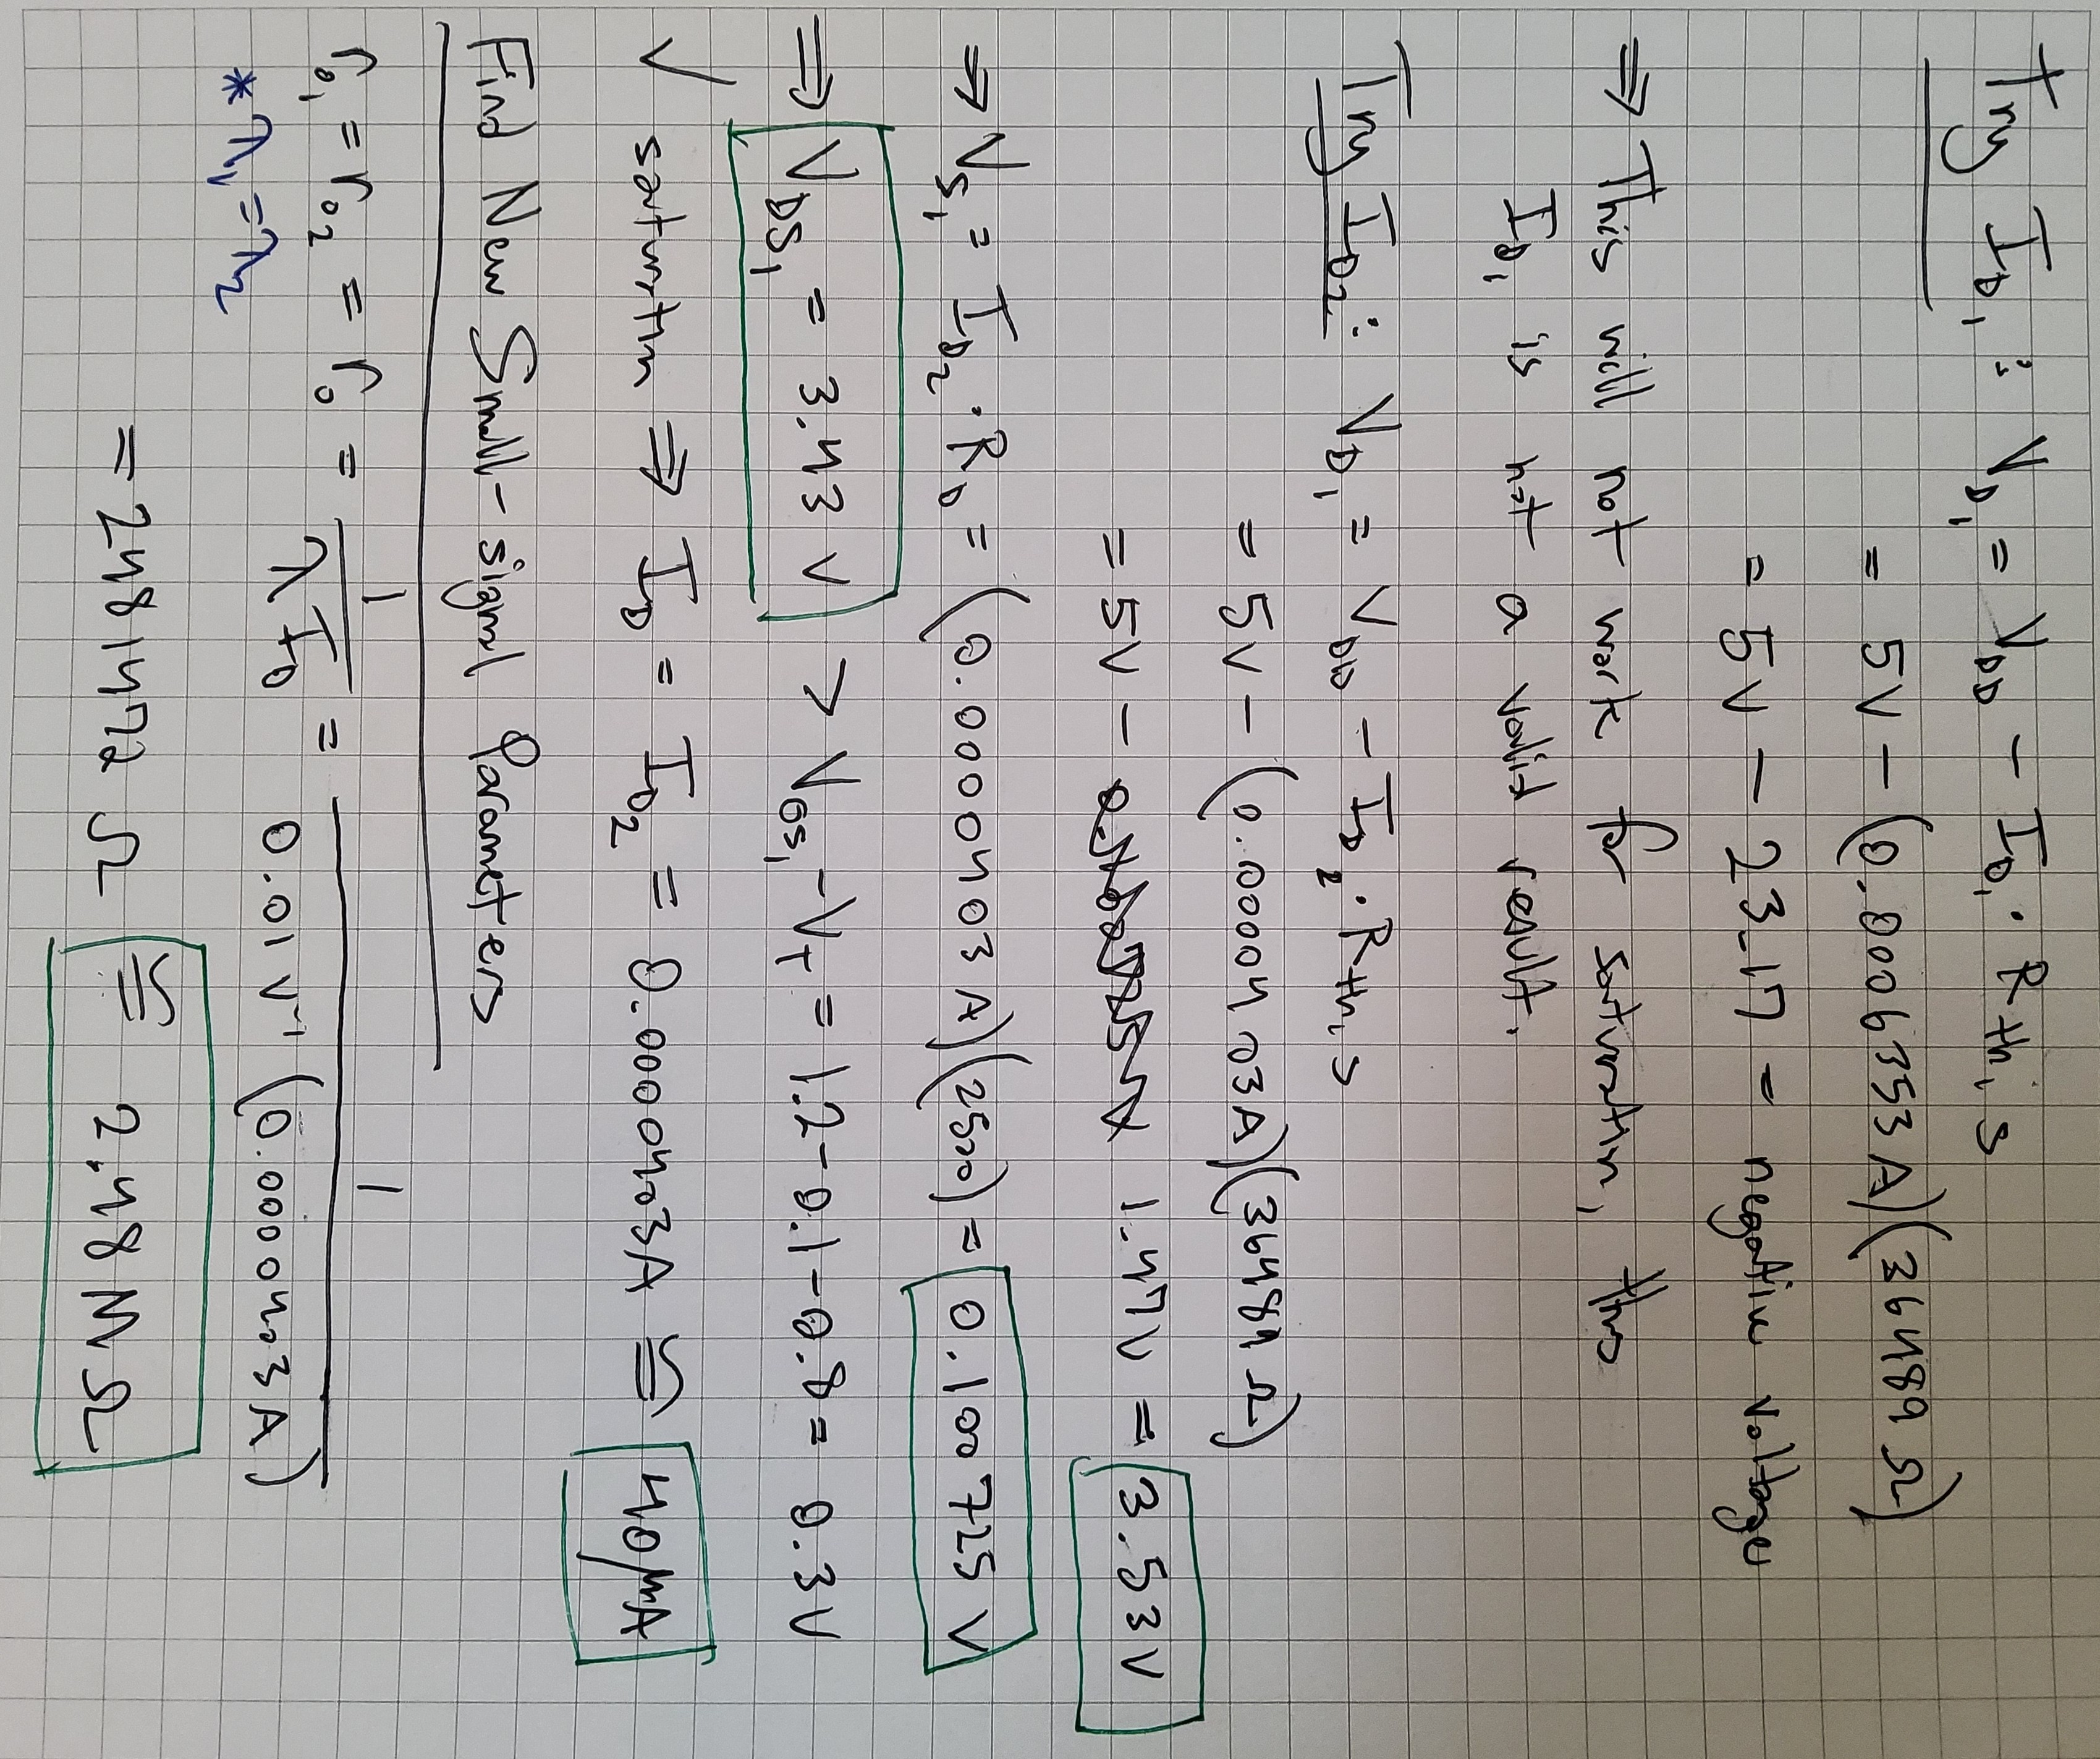
\includegraphics[scale=0.165, angle=90, center]{p1_8.jpg}\\
\newpage
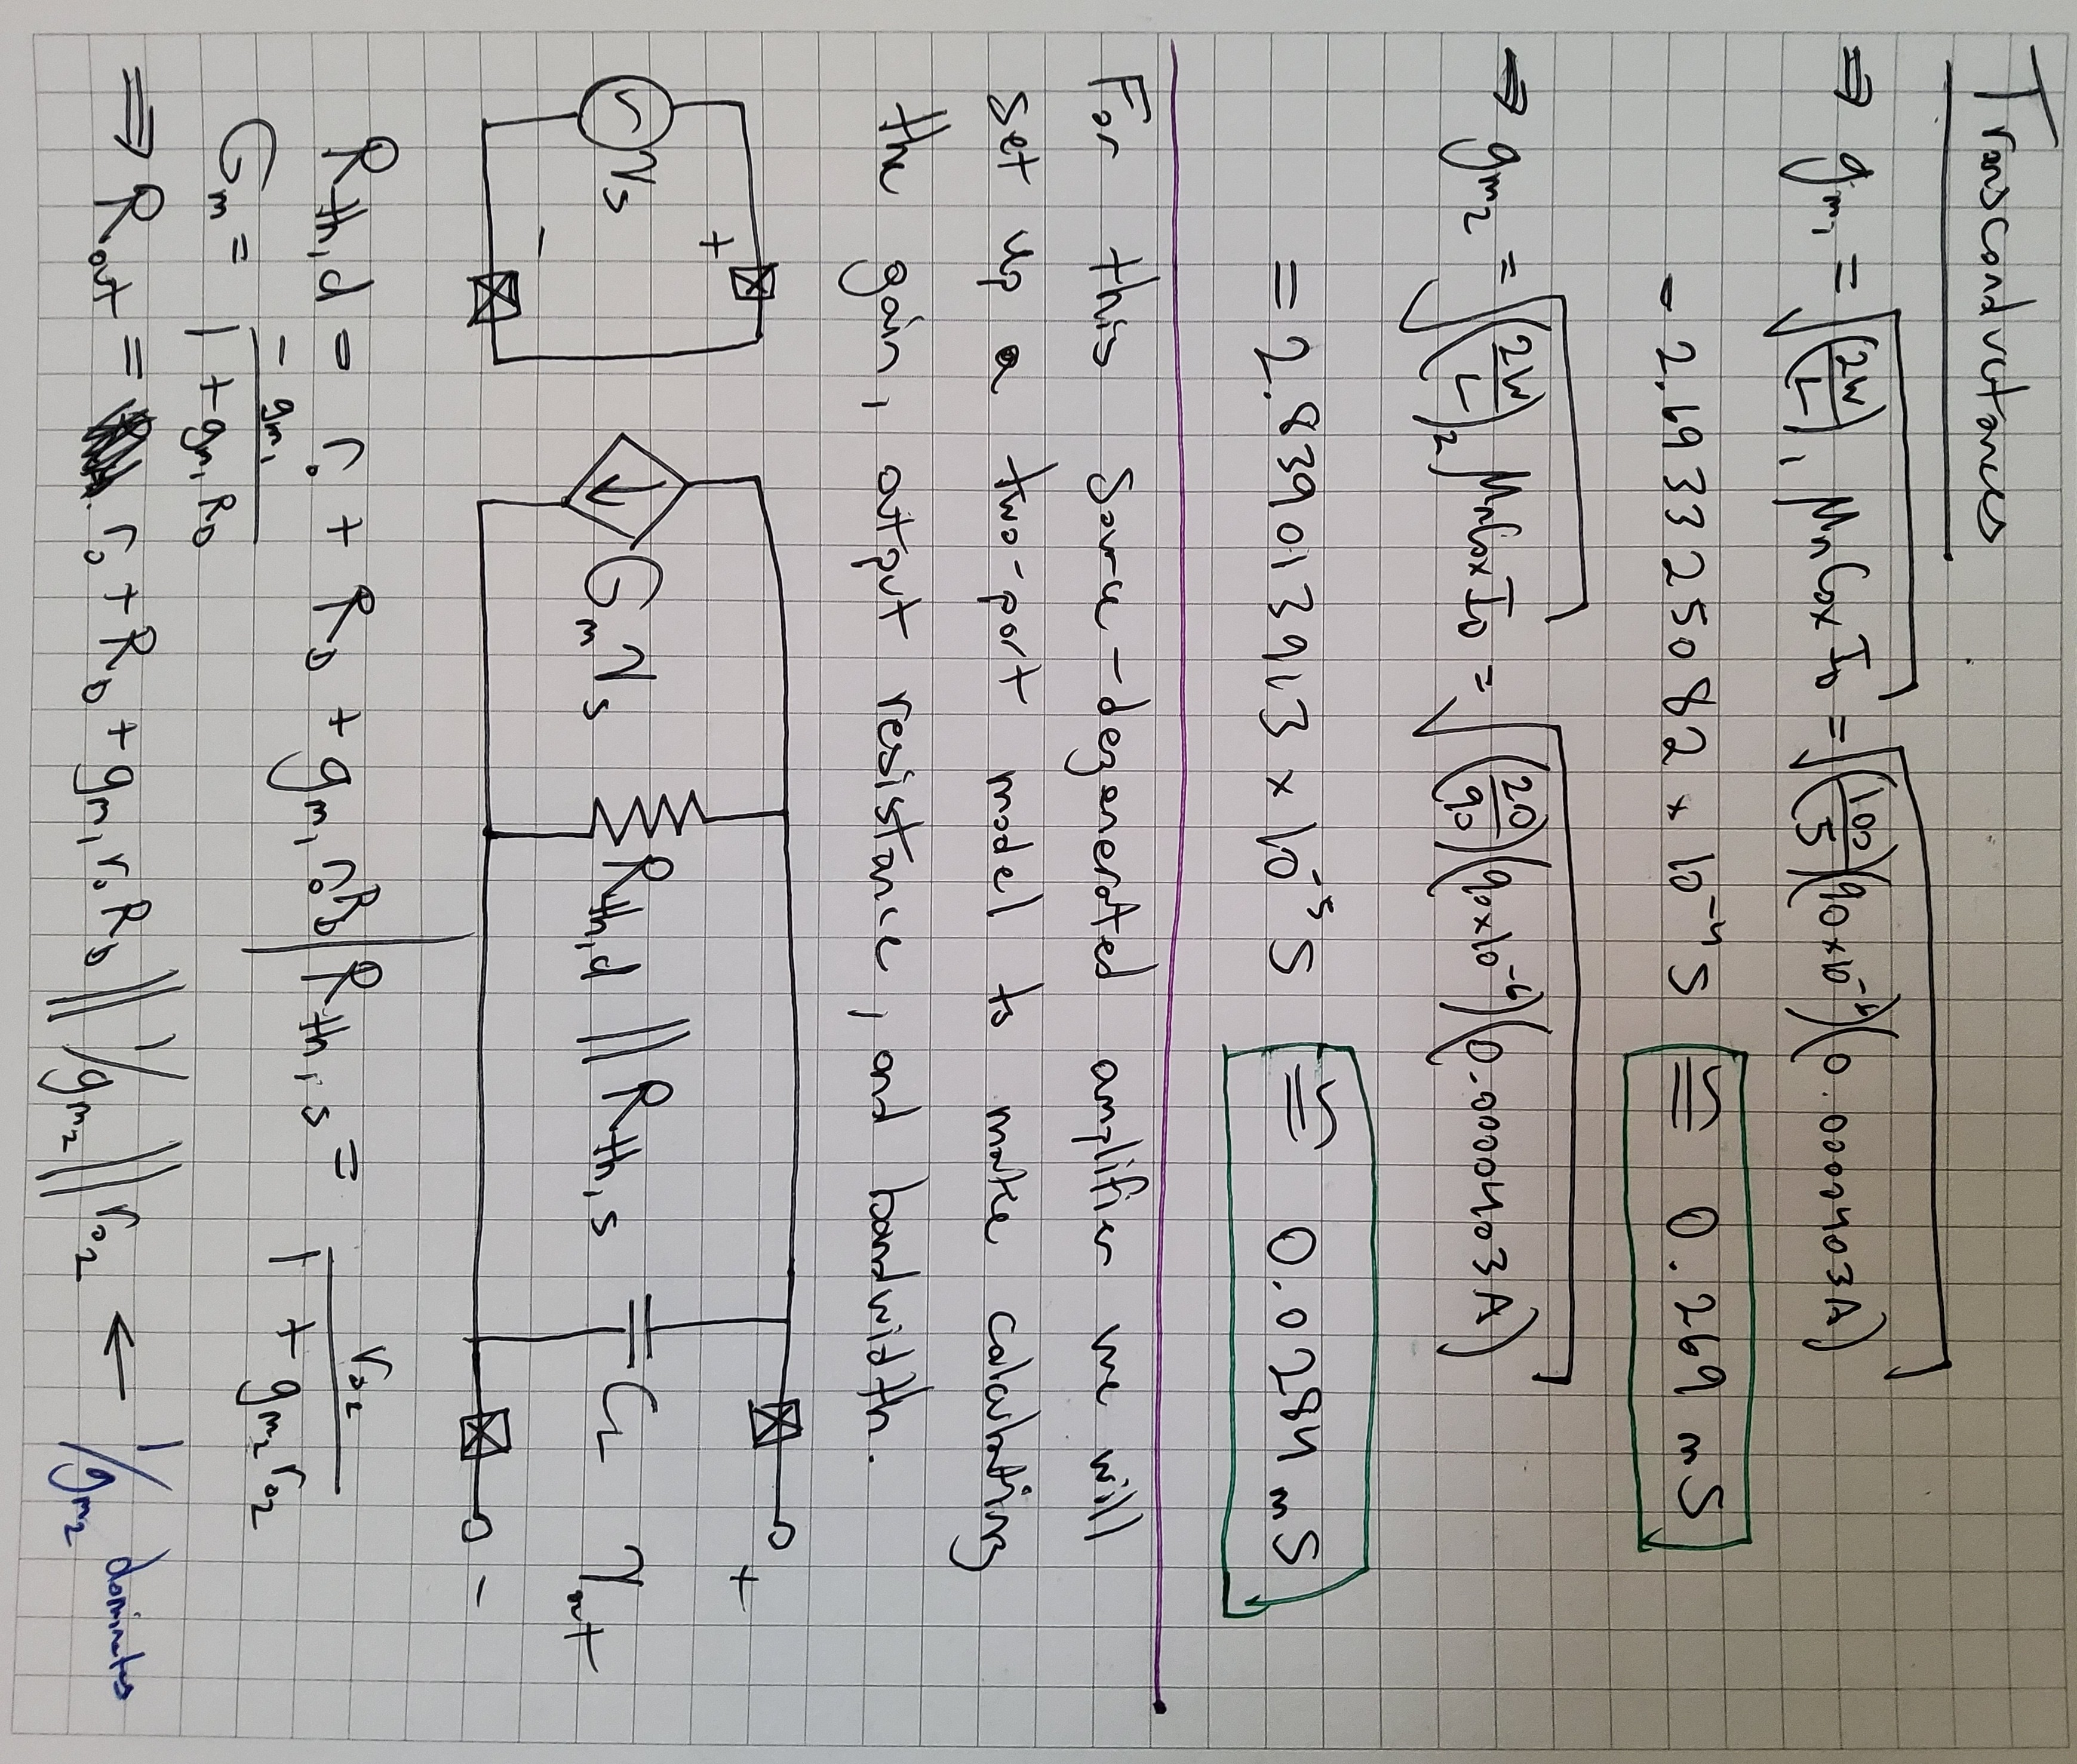
\includegraphics[scale=0.165, angle=90, center]{p1_9.jpg}\\
\newpage
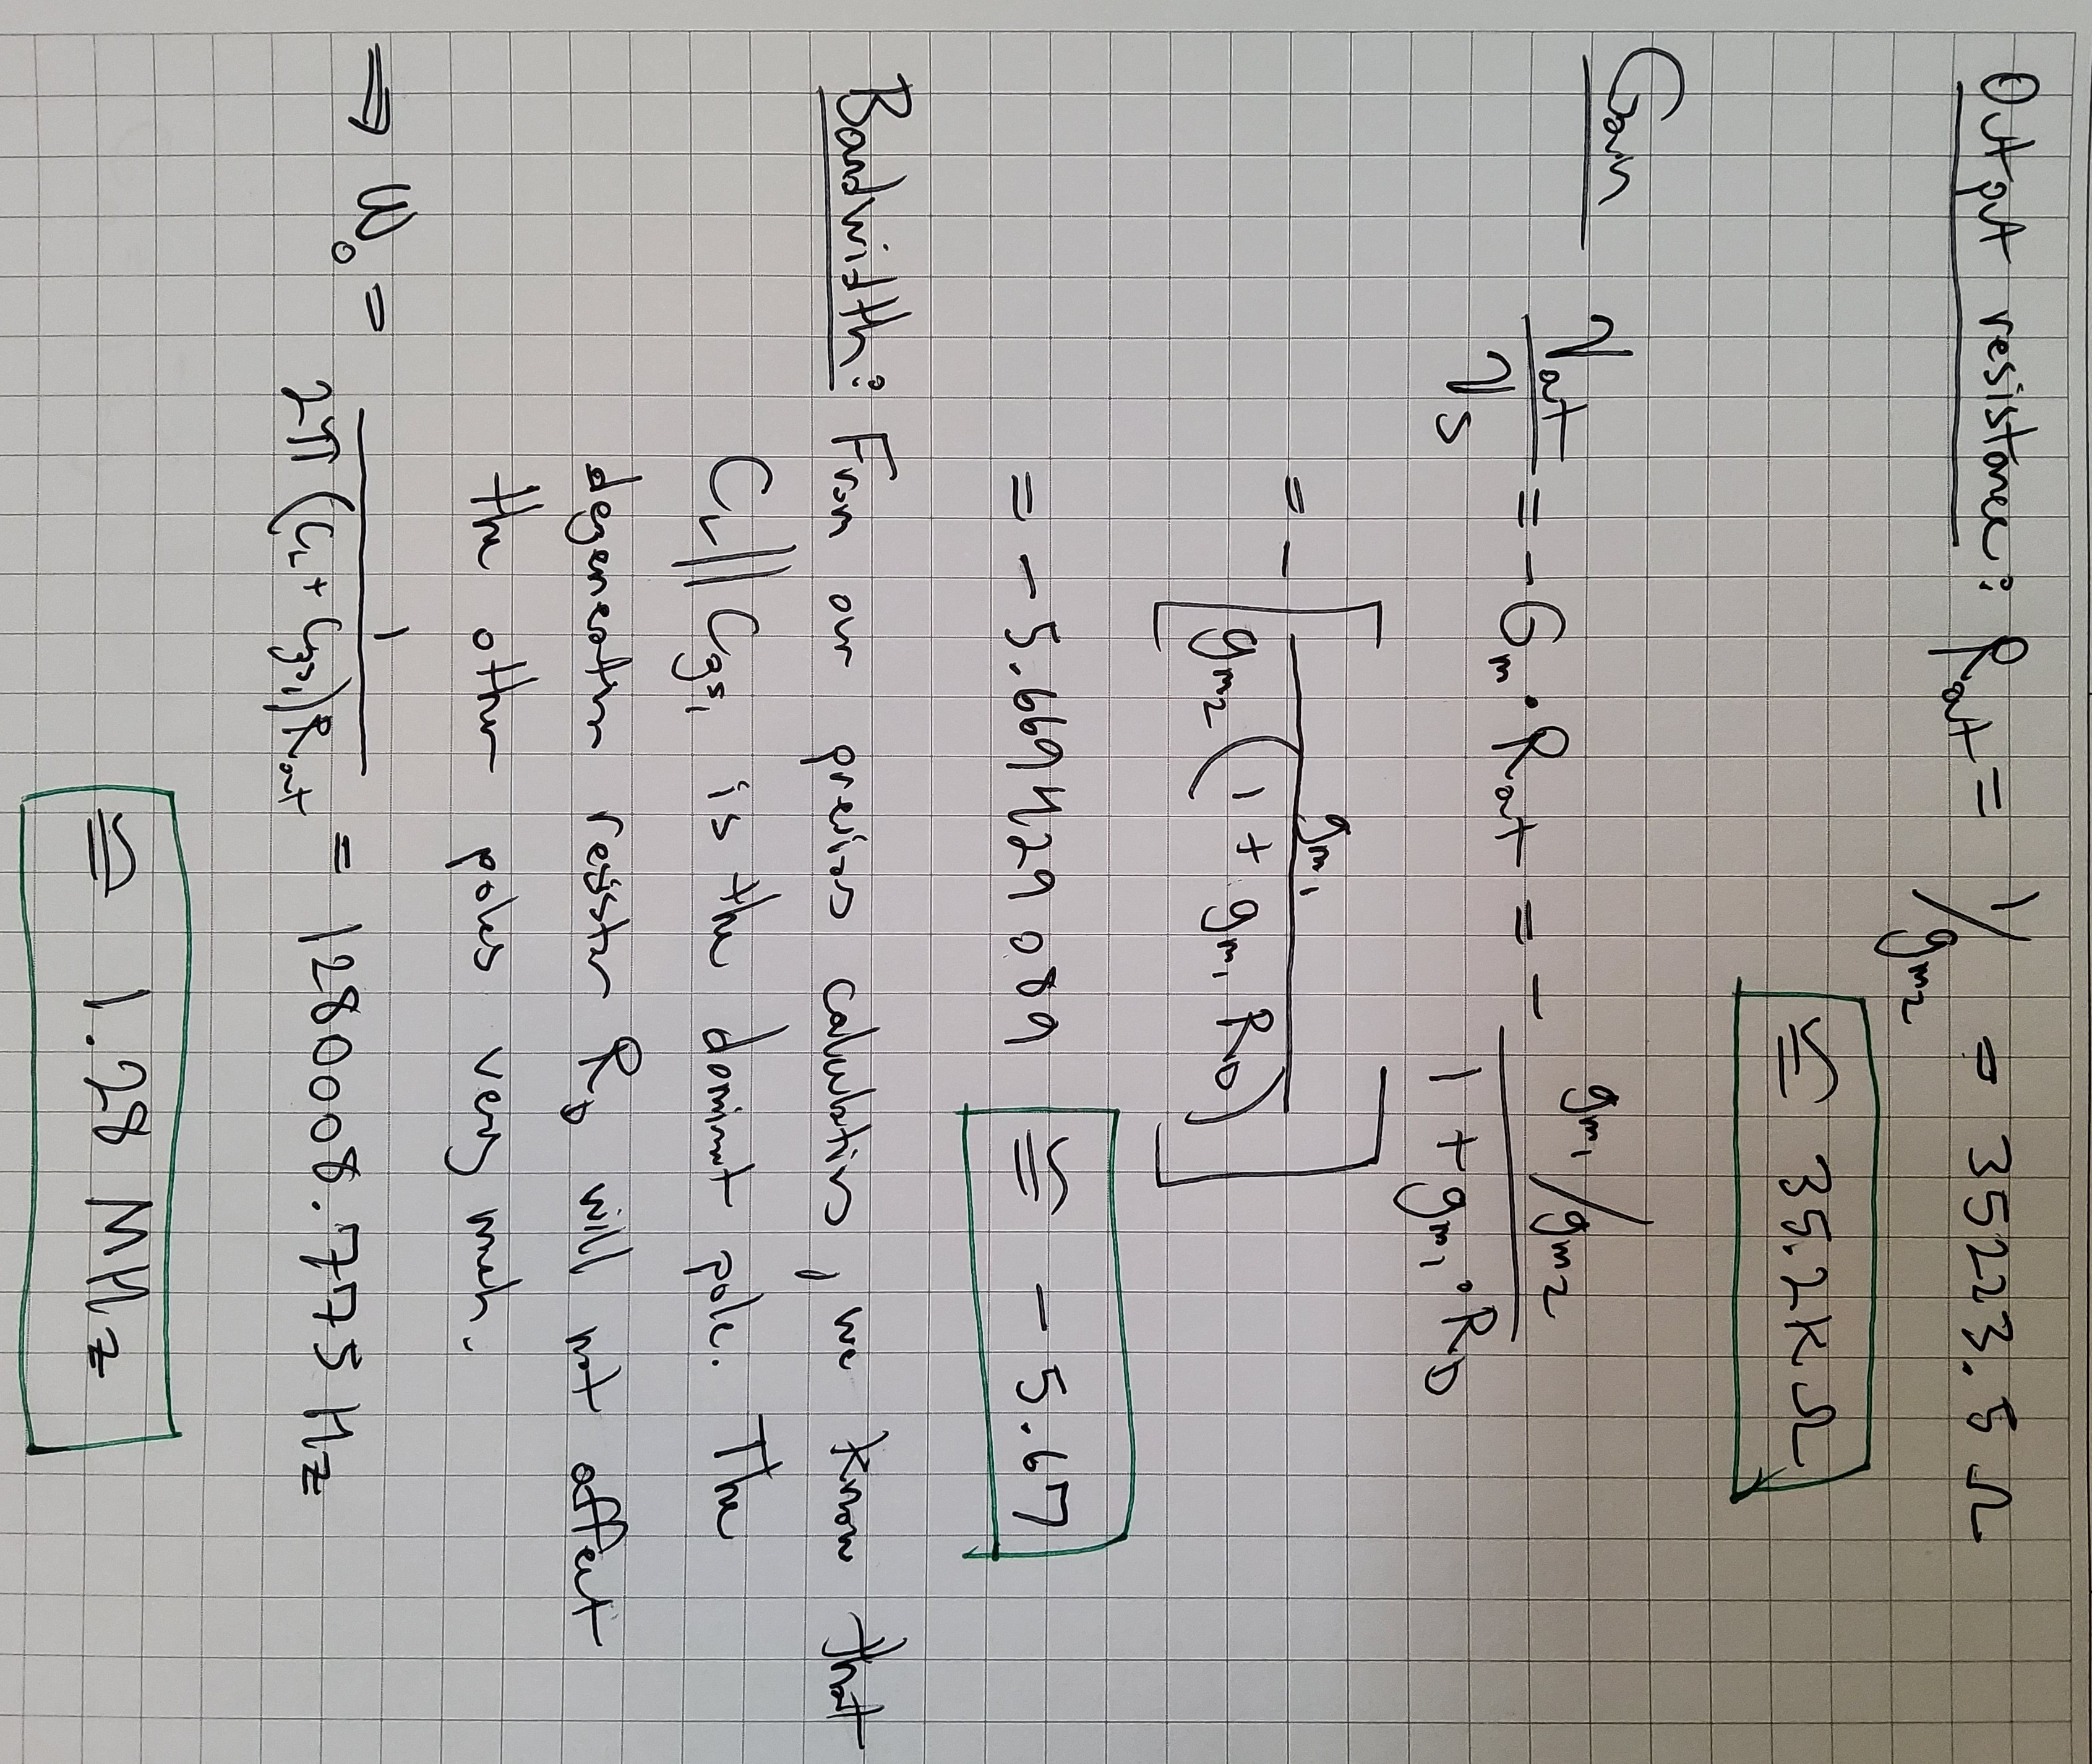
\includegraphics[scale=0.165, angle=90, center]{p1_10.jpg}\\
\newpage
%%%%%%%%%%%%%%%%%%%%%%%%%%%%%%%%%%%%%%%%
%               SIMULATION             %
%%%%%%%%%%%%%%%%%%%%%%%%%%%%%%%%%%%%%%%%
\subsubsection{Simulation}
The schematics have also not changed.  The values were changed accordingly to add source degeneration.
\begin{enumerate}
    \item
    {
    \textbf{\underline{Voltage Gain and Bandwidth}}\\[0.25cm]
    Below is the plot of the magnitude of the gain for the amplifier:\\[0.1cm]
    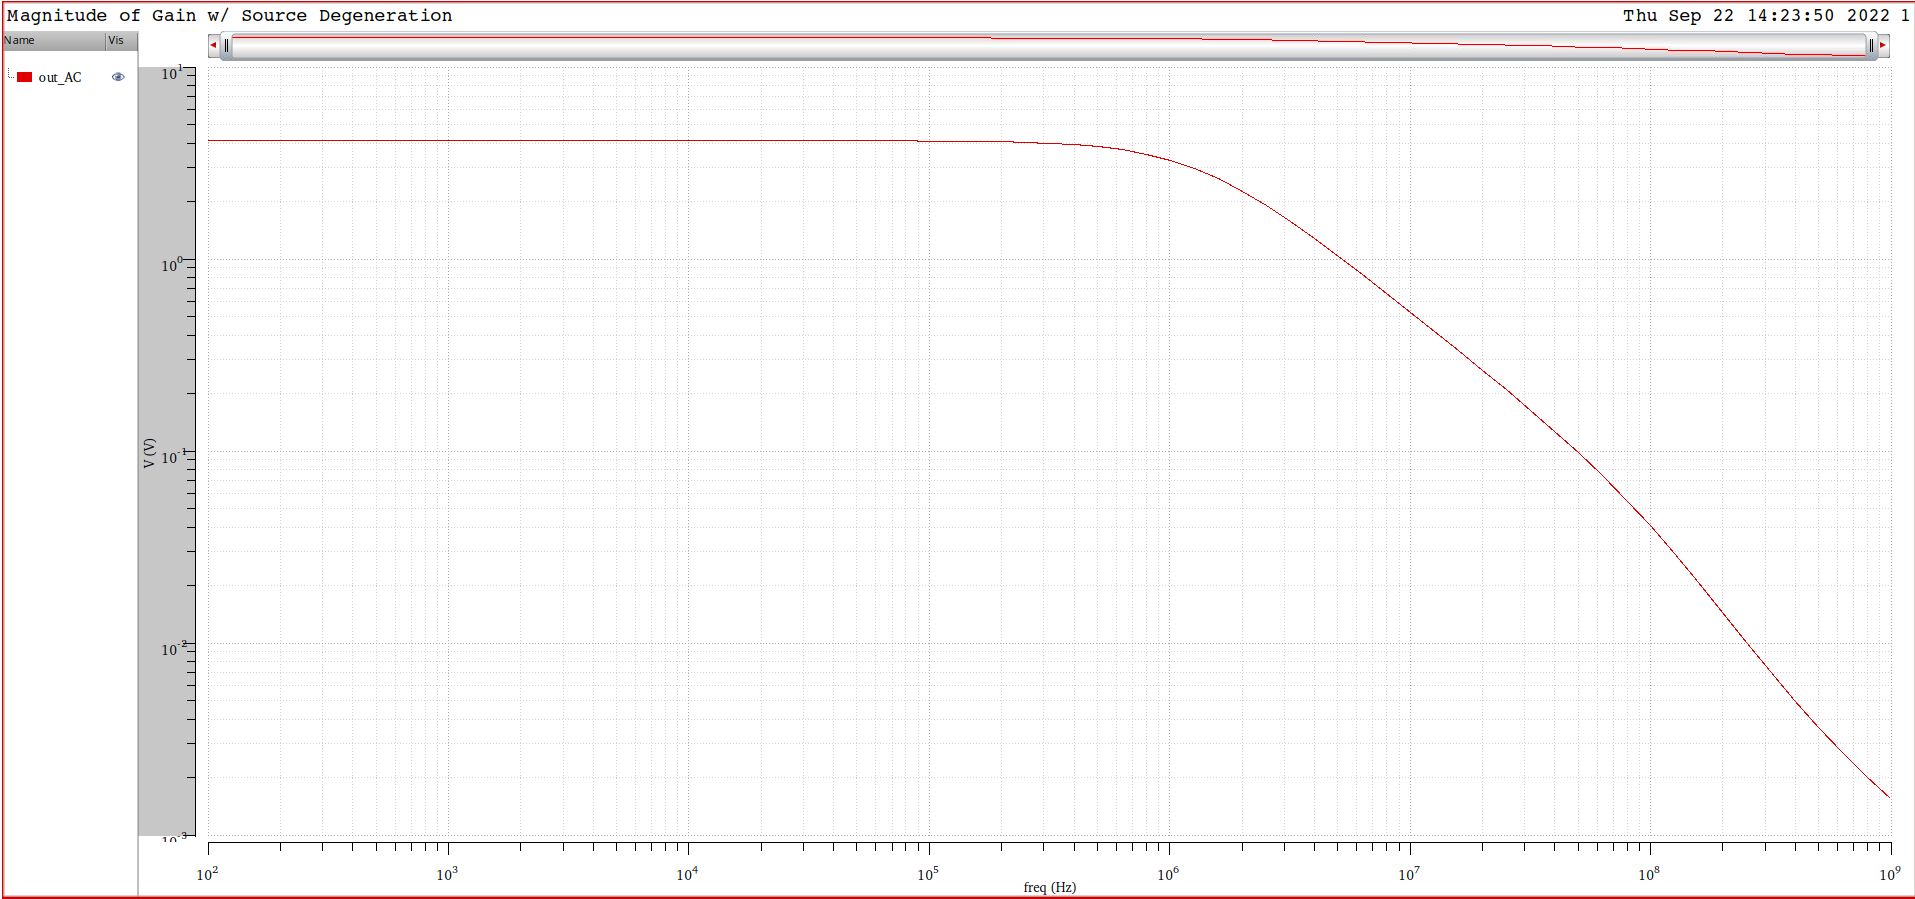
\includegraphics[scale=0.35, center]{b_plot.png}\\[0.5cm]
    Below are the simulated values for the voltage gain and bandwidth:\\[0.1cm]
    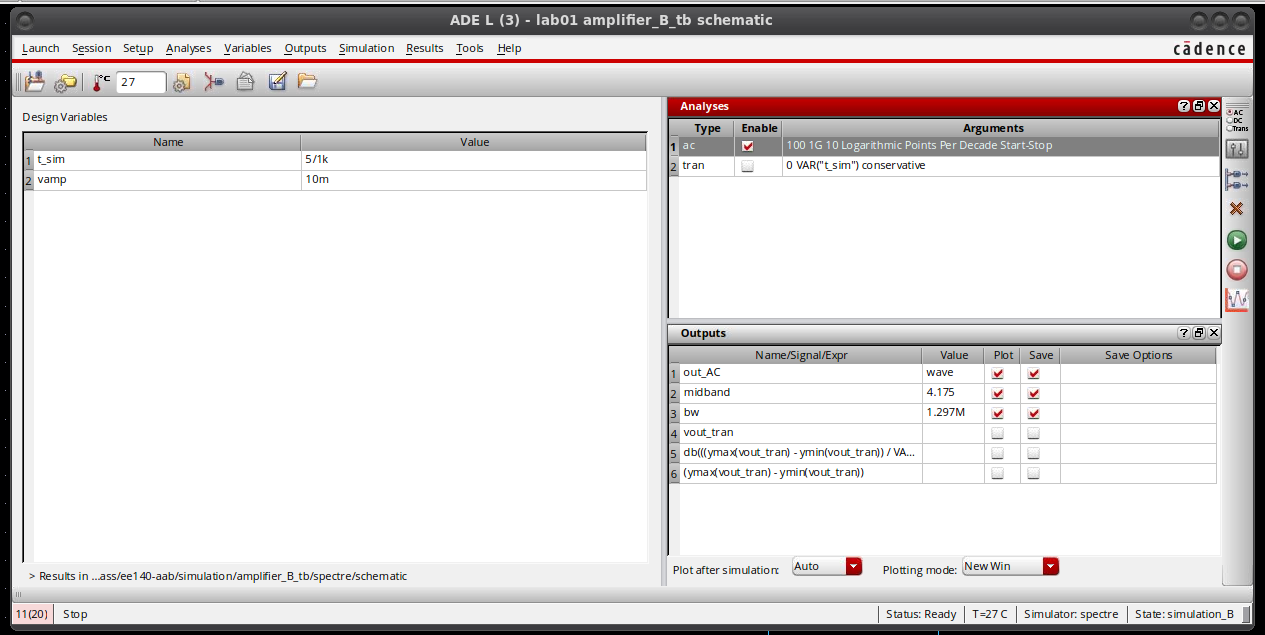
\includegraphics[scale=0.55, center]{b_gbw.png}\\
    }
    \newpage
    \item
    {
    \textbf{\underline{Output Resistance}}\\[0.25cm]
    Below is the simulated value of the output resistance using transient analysis:\\[0.1cm]
    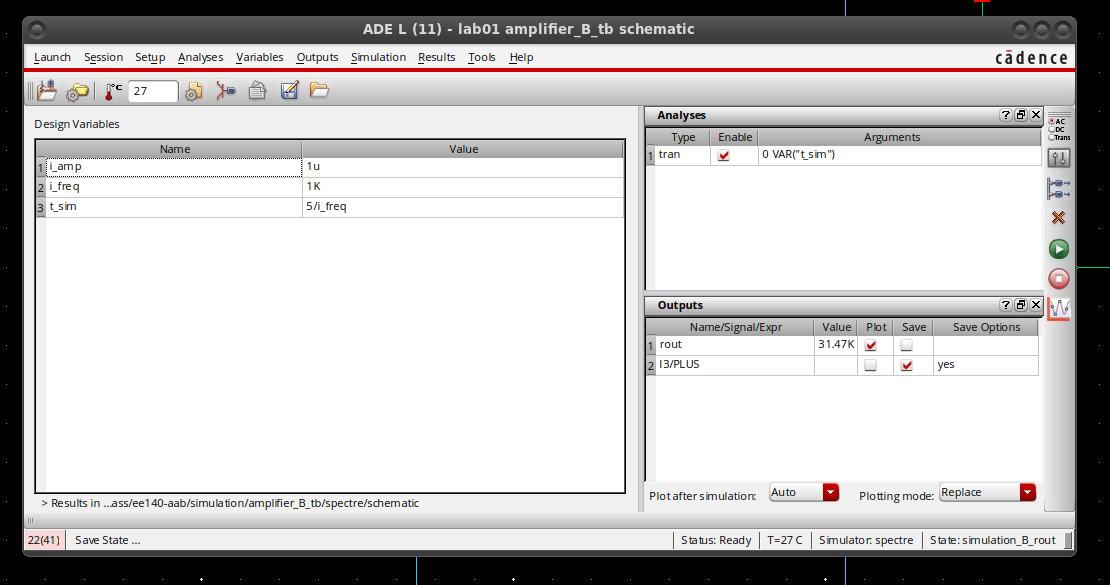
\includegraphics[scale=0.5, center]{b_rout.png}\\[0.5cm]
    }
    \item
    {
    \textbf{\underline{Output Voltage Swing}}\\[0.25cm]
    Below is the simulated value of the output voltage swing using the $1\,dB$ compression point:\\[0.1cm]
    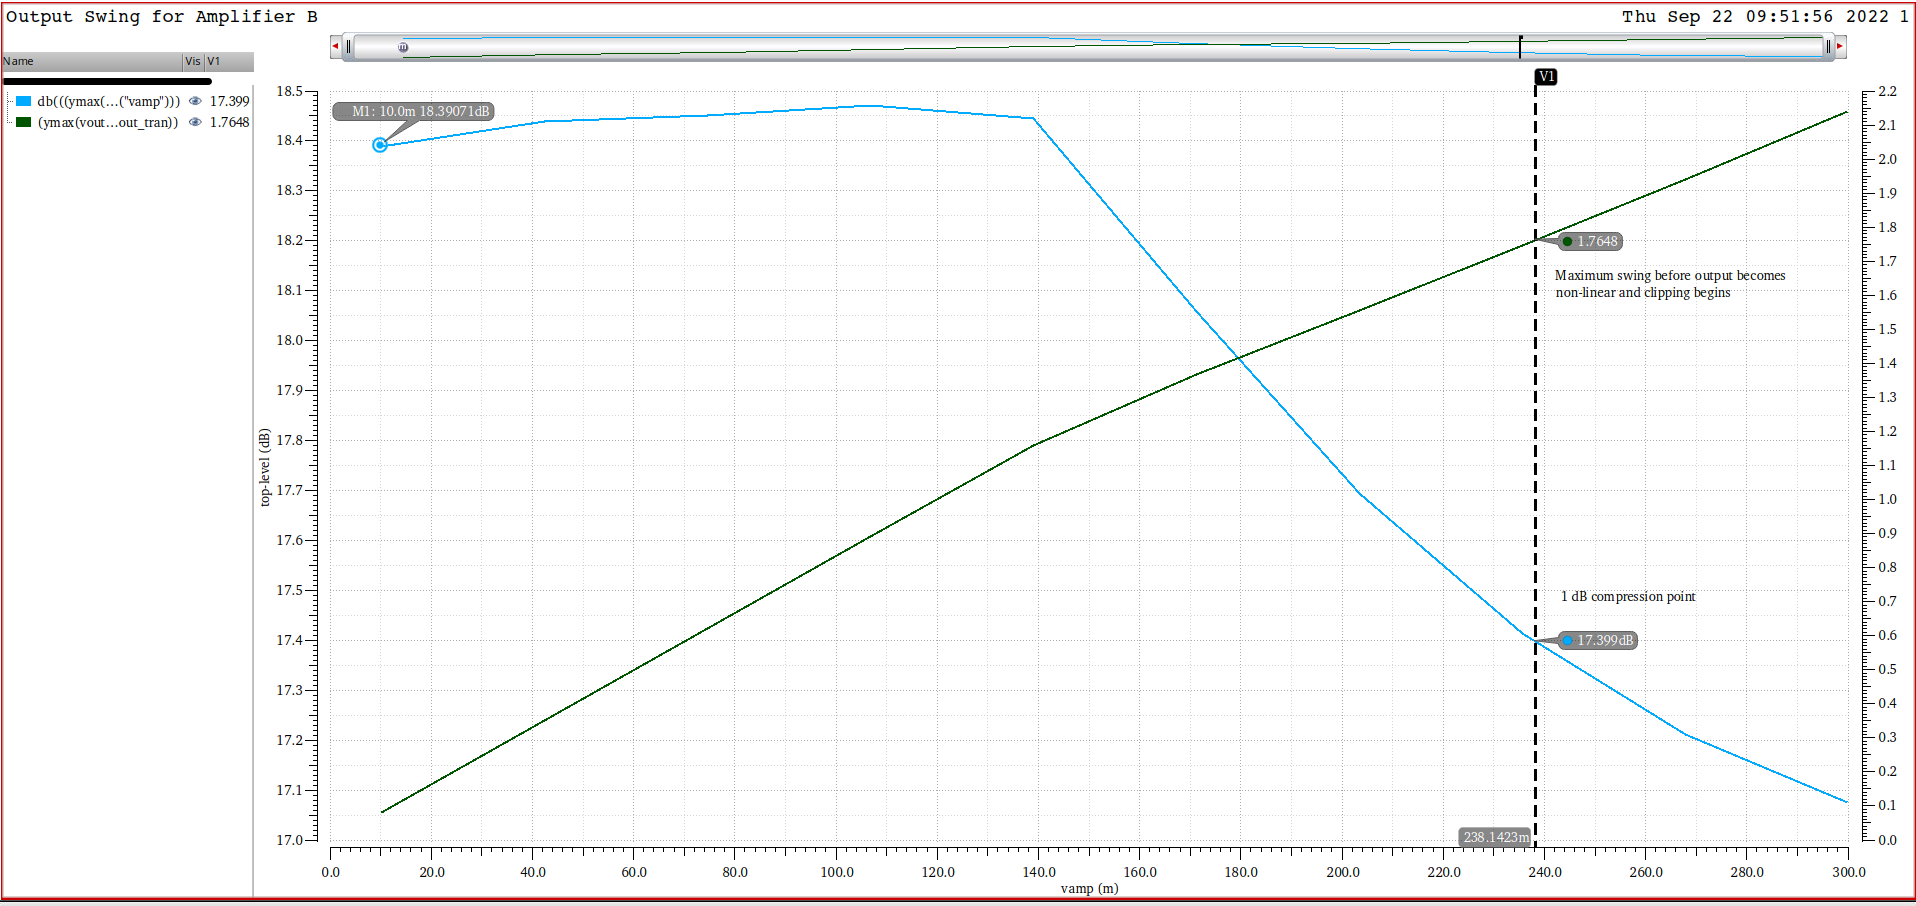
\includegraphics[scale=0.35, center]{b_swing.png}\\[0.5cm]
    }
\end{enumerate}
\newpage
%%%%%%%%%%%%%%%%%%%%%%%%%%%%%%%%%%%%%%%%
%                 RESULTS              %
%%%%%%%%%%%%%%%%%%%%%%%%%%%%%%%%%%%%%%%%
\subsubsection{Results}
Below is a table of results for both the hand calculations and simulated values:

\begin{table}[H]
\centering
\setlength{\tabcolsep}{20pt}
\renewcommand{\arraystretch}{1.5}
\begin{tabular}{|l|c|c|}
    \hline
    \textbf{\textit{Parameter}} & \textbf{\textit{Hand Calculated Value}} & \textbf{\textit{Simulated Value}}\\
    \hline
    $\left|\text{\textit{Voltage Gain}}\right|$ & $5.67\,V/V$ & $4.175\,V/V$\\
    \hline
    \textit{Bandwidth} & $1.28\,MHz$ & $1.297\,MHz$\\
    \hline
    \textit{Output Resistance} & $35.2\,k\Omega$ & $31.47\,k\Omega$\\
    \hline
    \textit{Voltage Swing} & X & $1.7648\,V$\\
    \hline
\end{tabular}
\caption{Results for amplifier in \textit{Task B}.}
\end{table}
\noindent
\underline{\textbf{\textit{Summary of Results}}}\\[0.25cm]
Here we see the same general trend of discrepancies in hand calculated values compared to the results of simulation as that of \textit{Task A}.  Because we also ignored the body effect and channel length modulation in the hand calculations of \textit{Task B}, the reasons for these discrepancies are due to the same reasons already described in the conclusion of results from \textit{Task A}.
%%%%%%%%%%%%%%%%%%%%%%%%%%%%%%%%%%%%%%%%%%%%%%%%%%%%%%%%%%%%%%%%%%%%%%%%%%%%%%%%%%%%%%%%%%%%%%%%%%%%%%%%%%%
%                                               PART 2                                                    %
%%%%%%%%%%%%%%%%%%%%%%%%%%%%%%%%%%%%%%%%%%%%%%%%%%%%%%%%%%%%%%%%%%%%%%%%%%%%%%%%%%%%%%%%%%%%%%%%%%%%%%%%%%%
\newpage
\section{Part II}
%%%%%%%%%%%%%%%%%%%%%%%%%%%%%%%%%%%%%%%%%%%%%%%%%%%%%%
%                       TASK A                       %
%%%%%%%%%%%%%%%%%%%%%%%%%%%%%%%%%%%%%%%%%%%%%%%%%%%%%%
\subsection{MOS Amplifier Design}
\textbf{\emph{Find: }}\\[0.25cm]\noindent
Design a common-source amplifier with a saturated $PMOS$ load as shown in the figure below:\\[0.25cm]
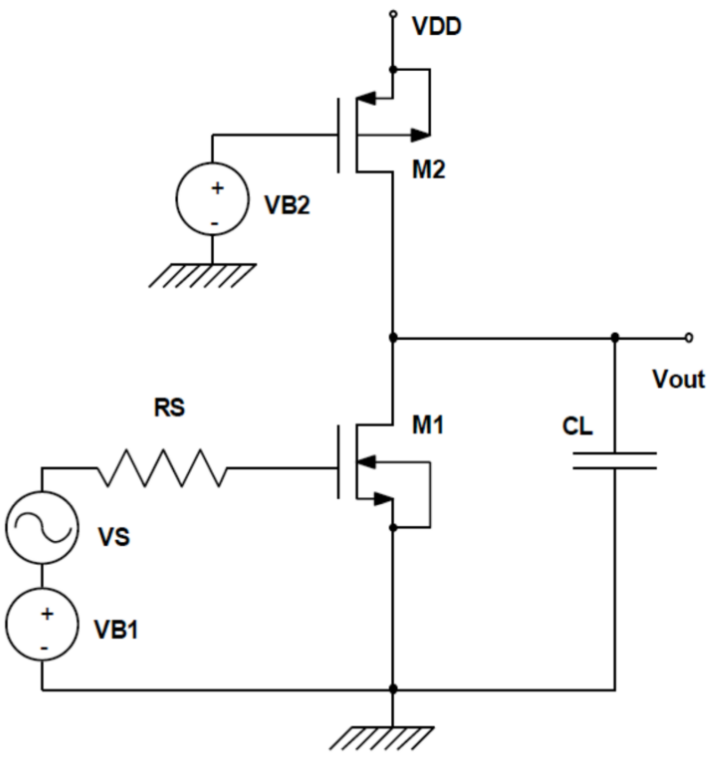
\includegraphics[scale=0.25, center]{p2pmos.PNG}\\
\noindent
Note that all biasing in this circuit is performed with two DC sources: $VB1$ and $VB2$. The power supply for this amplifier is $V_{DD} = 5\,V$. In your design, you have to determine the values of these two sources. There are two external elements in this amplifier:
\begin{align*}
    R_S &= 5\,k\Omega\\[0.25cm]
    C_L &= 2.5\,pF
\end{align*}
Design the above common-source amplifier so that it satisfies the following specifications:
\begin{table}[H]
\centering
\setlength{\tabcolsep}{20pt}
\renewcommand{\arraystretch}{1.5}
\begin{tabular}{|l|c|}
    \hline
    \textit{\textbf{Parameter}} & \textit{\textbf{Specification}}\\
    \hline
    \textit{Midband Gain} & $\geq 120\,V/V$\\
    \hline
    \textit{$3\,dB$ Cutoff Frequency (bandwidth)} & $\geq 180\,kHz$\\
    \hline
    \textit{Output Voltage Swing} & $\geq 3\,V_{pp}$\\
    \hline
    \textit{Load Capacitance} & $2.5\,pF$\\
    \hline
    \textit{Source Resistance} & $5\,k\Omega$\\
    \hline
    \textit{Supply Voltage} & $V_{DD} = 5\,V,\;V_{SS} = 0\,V$\\
    \hline
\end{tabular}
\caption{CS amplifier specifications.
\label{tab:cs_specs}} 
\end{table}
\newpage\noindent
\textbf{\emph{Solution: }}
%%%%%%%%%%%%%%%%%%%%%%%%%%%%%%%%%%%%%%%%
%            HAND CALCULATIONS         %
%%%%%%%%%%%%%%%%%%%%%%%%%%%%%%%%%%%%%%%%
\subsubsection{Hand Calculations}
For the hand calculations we will again be ignoring the body effect and channel length modulation.  We will also assume that $C_L$ is the dominant pole, which will be checked in the hand calculations to make sure our assumption was correct.\\[0.25cm]
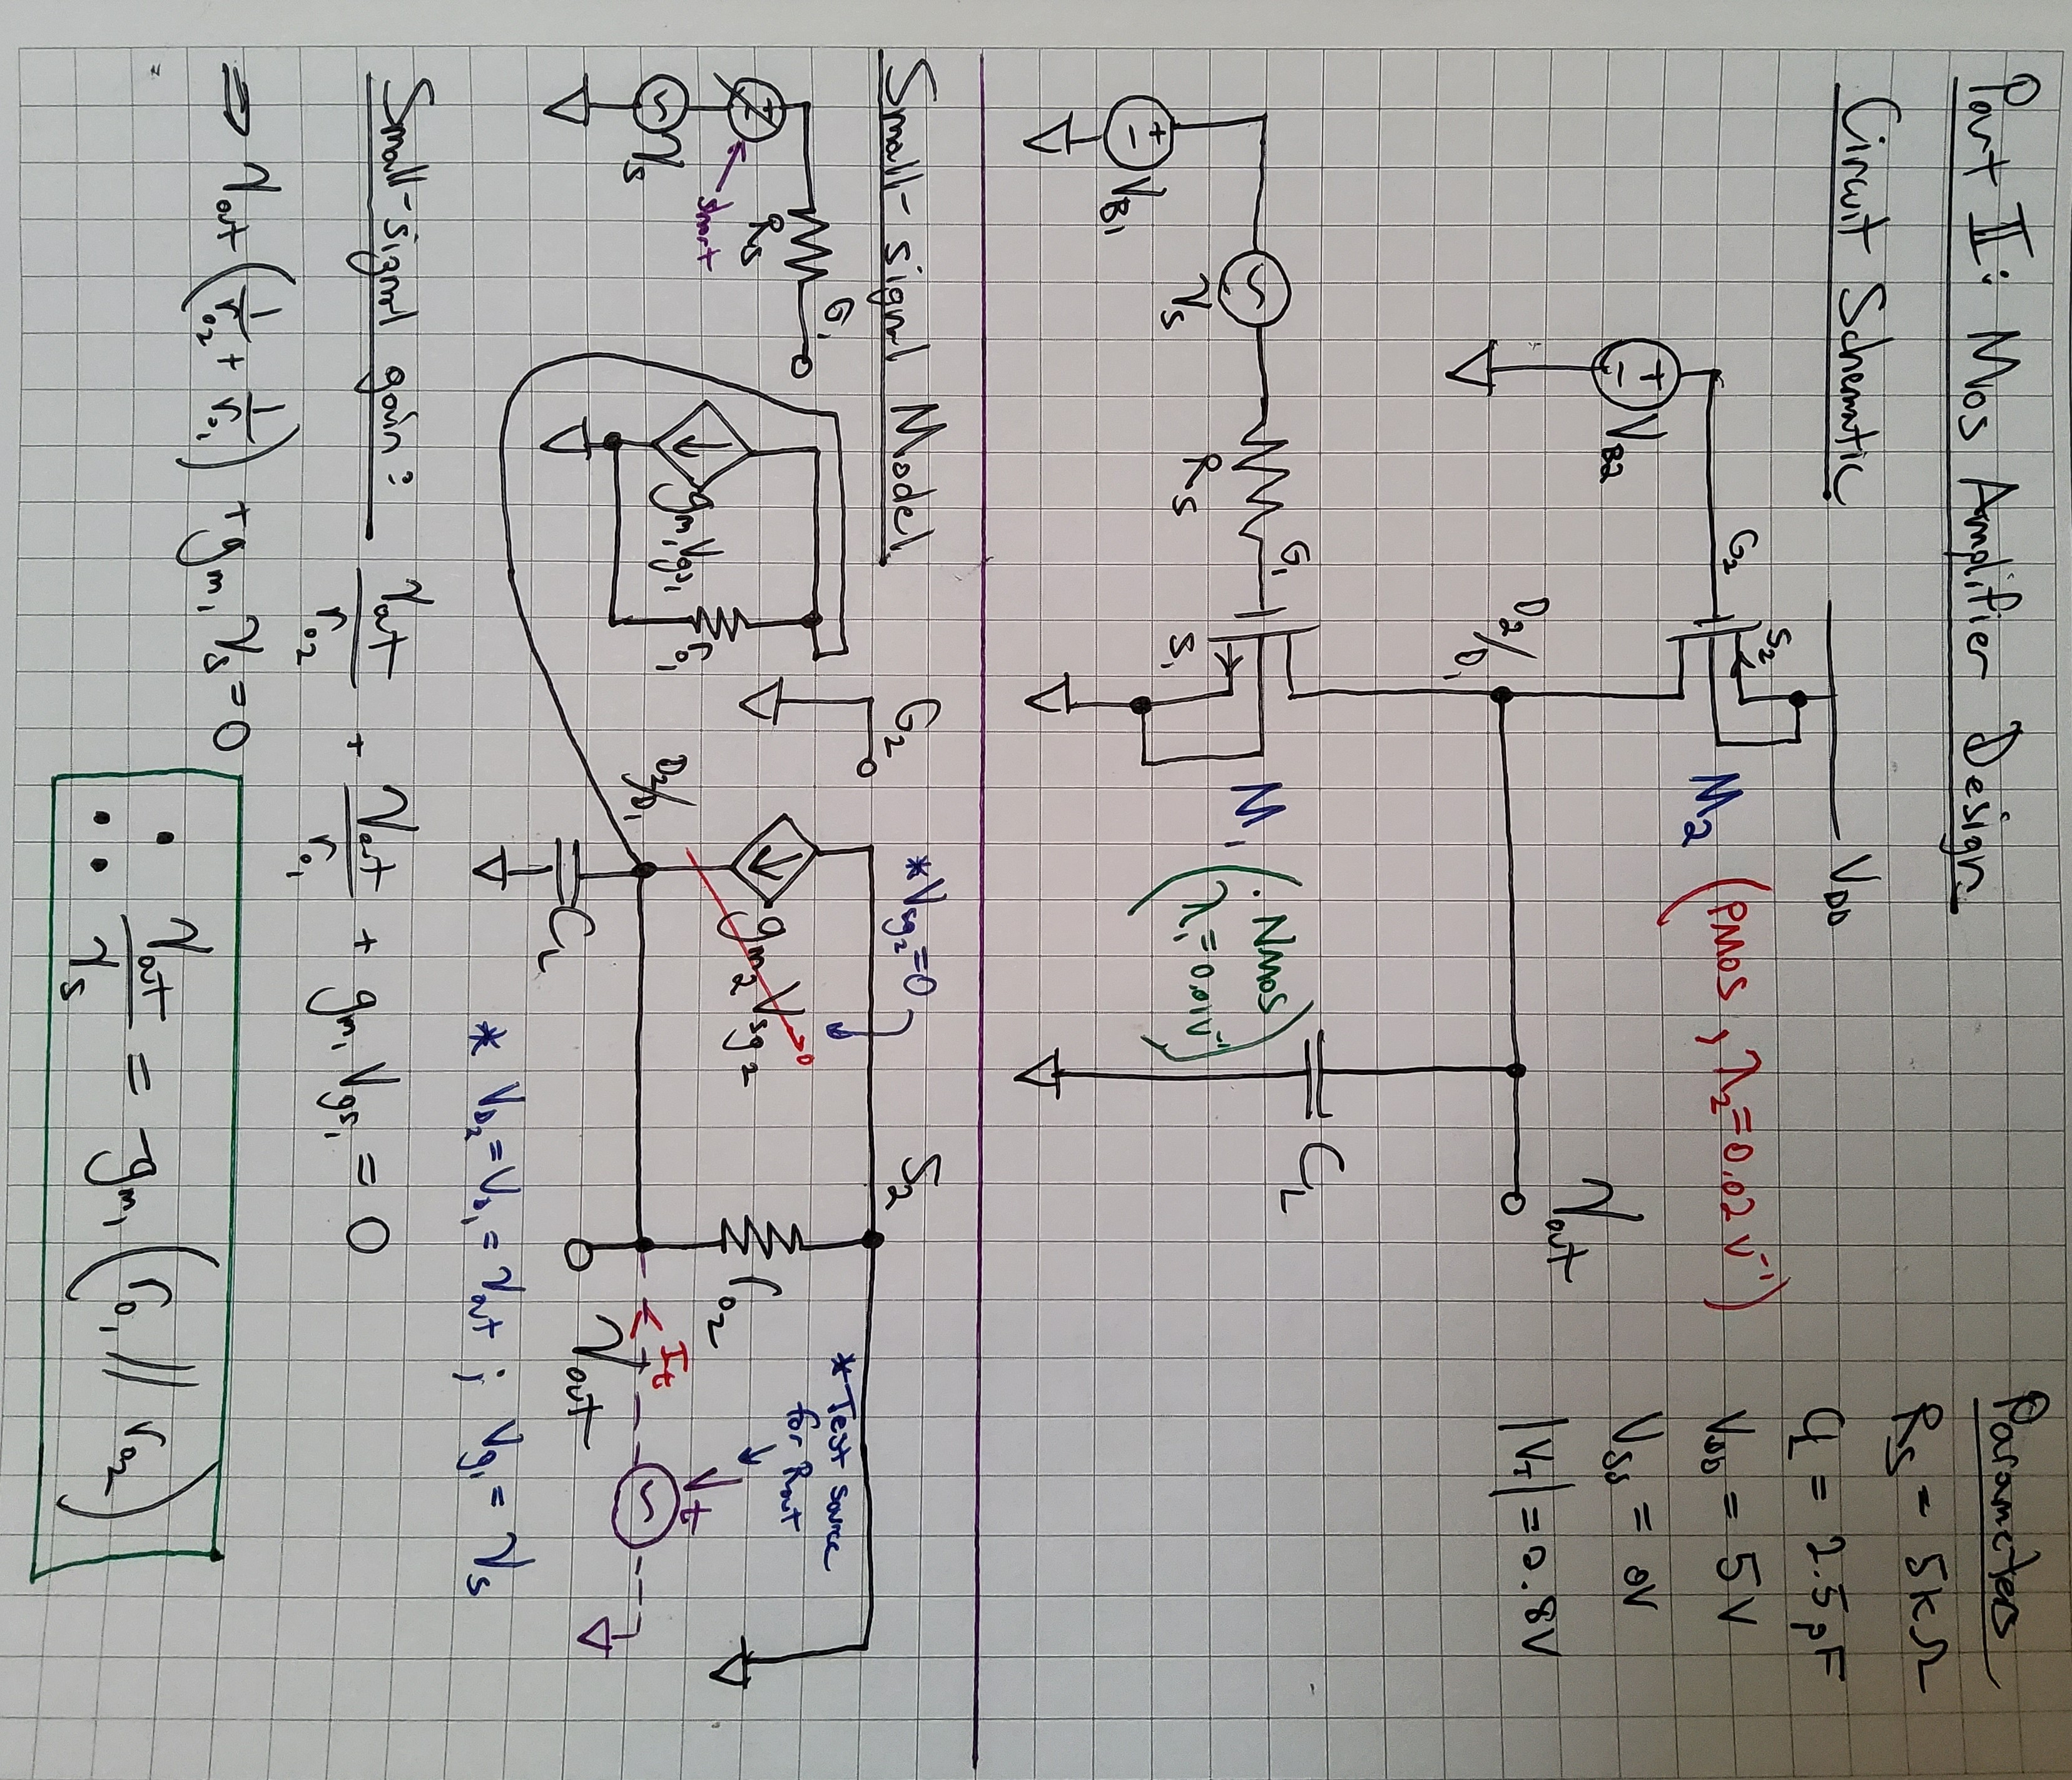
\includegraphics[scale=0.155, angle=90, center]{p2a_1.jpg}\\
\newpage
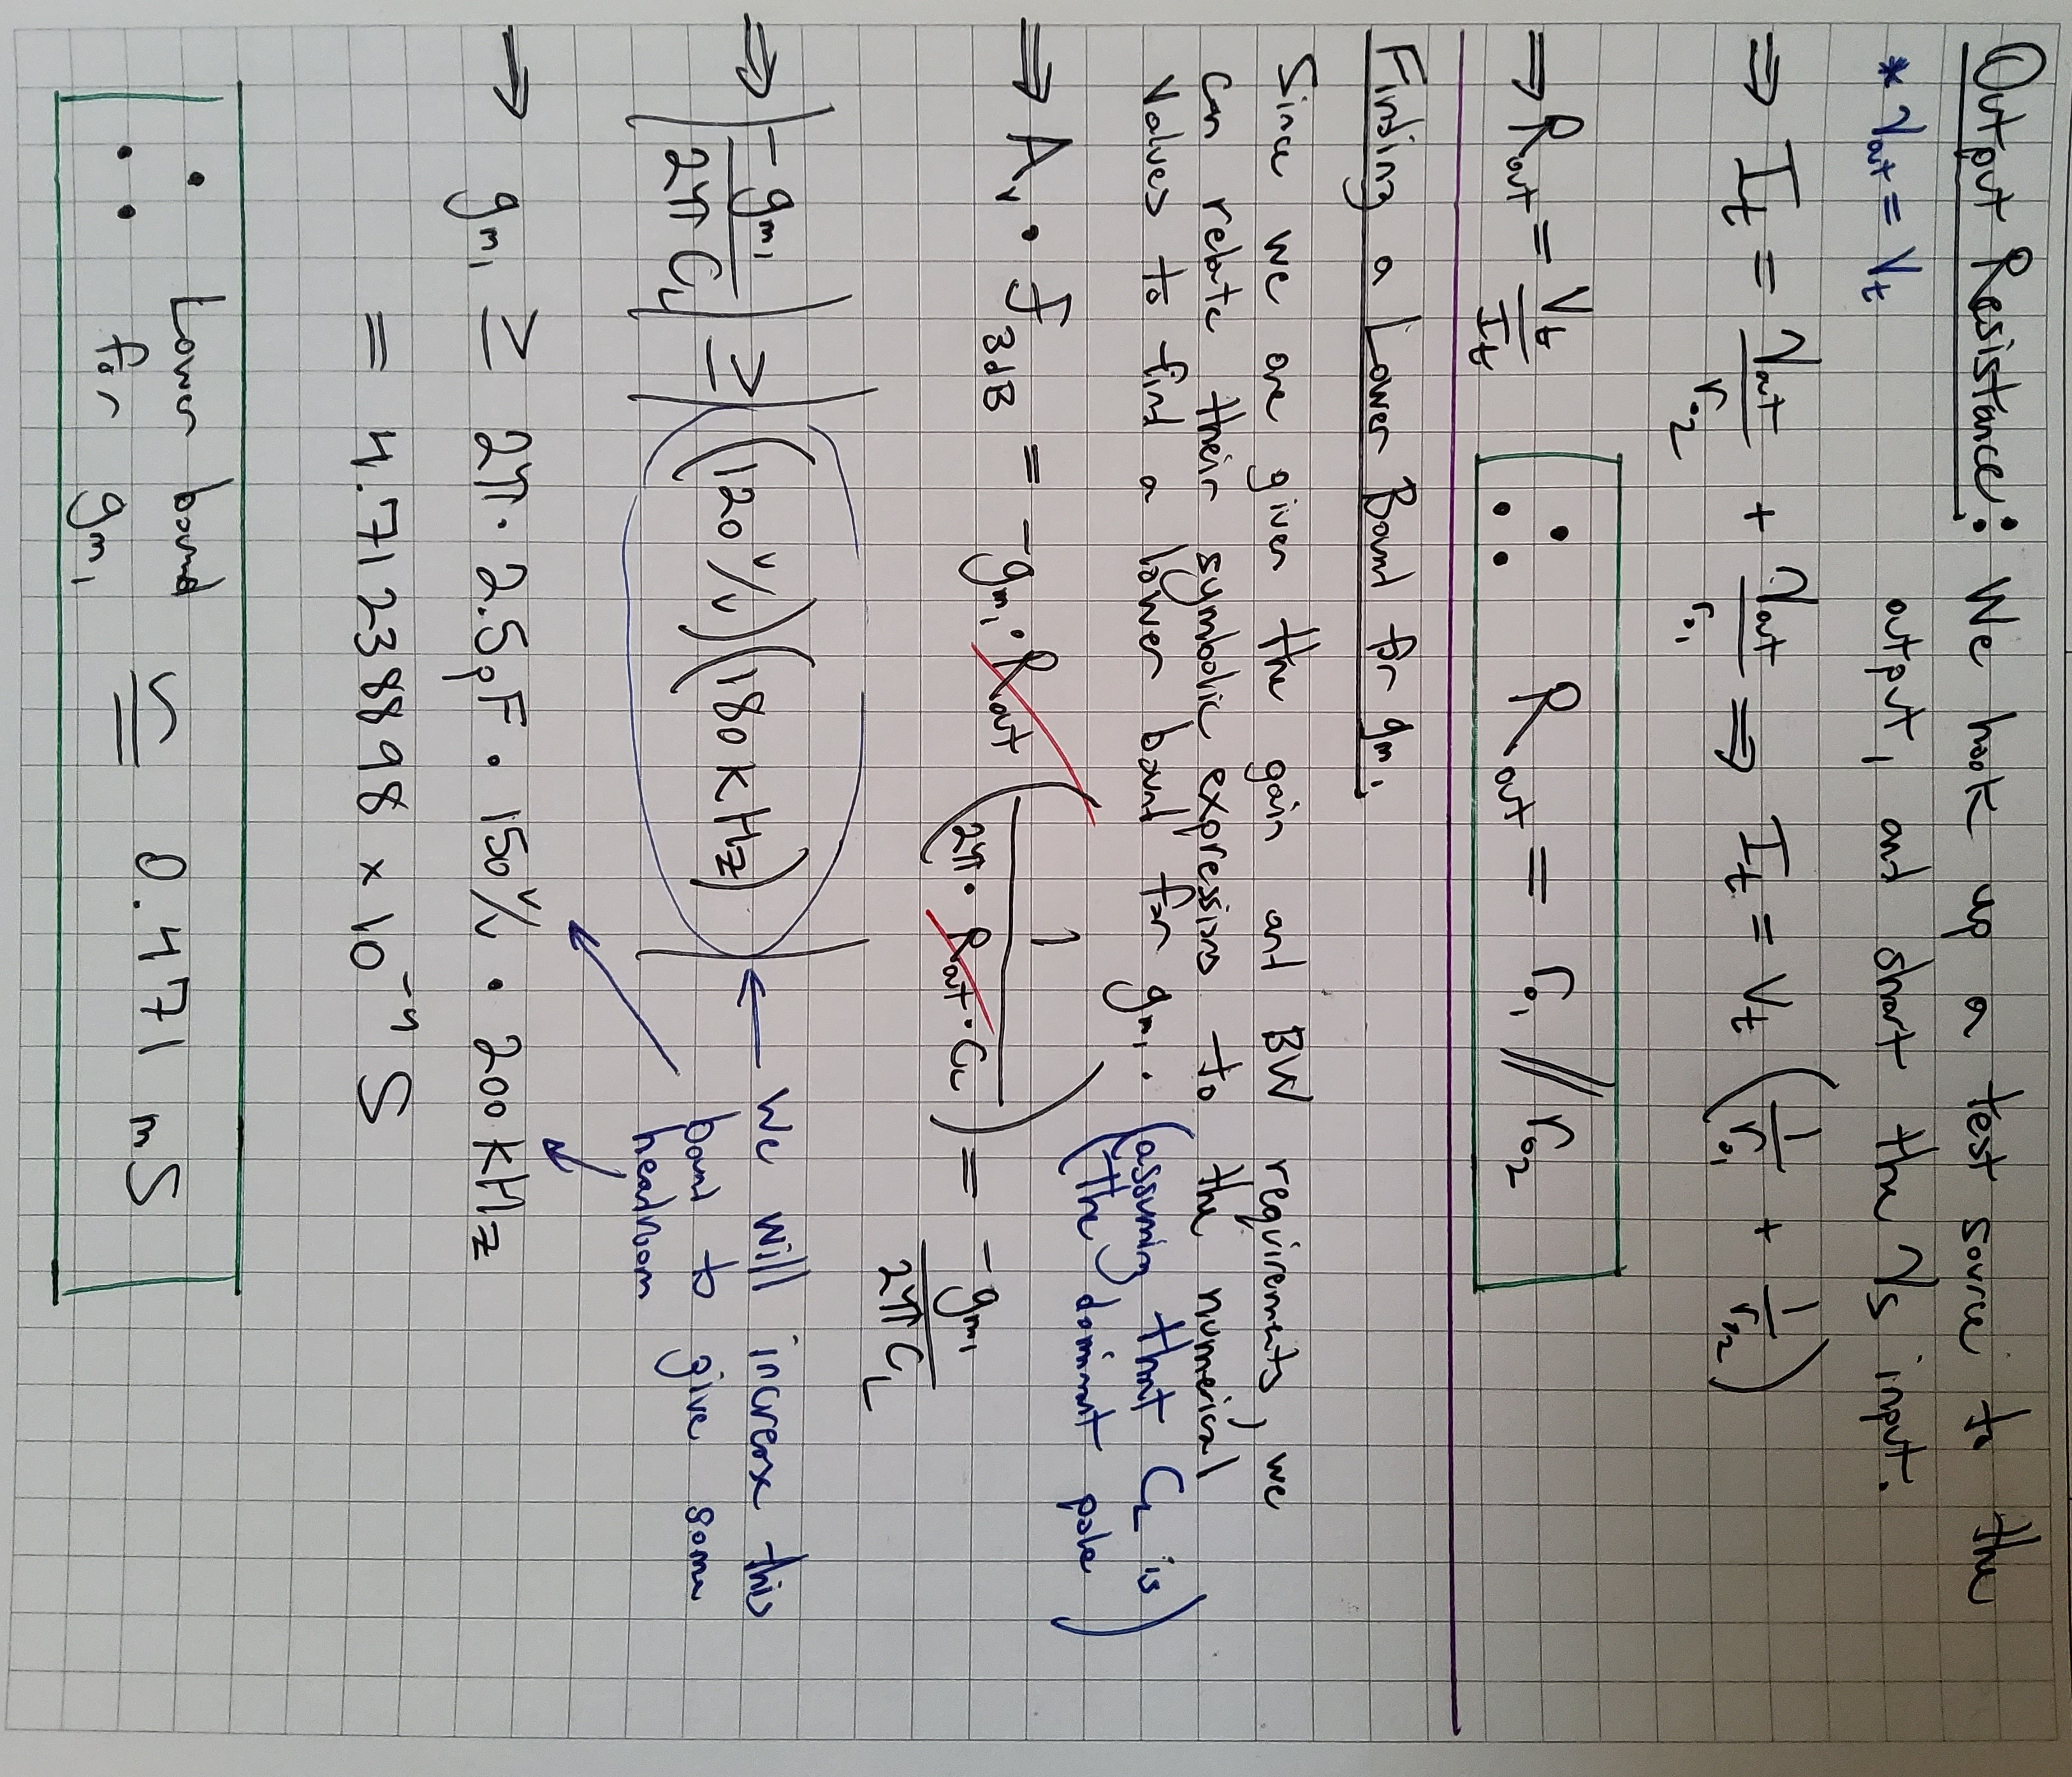
\includegraphics[scale=0.165, angle=90, center]{p2a_2.jpg}\\
\newpage
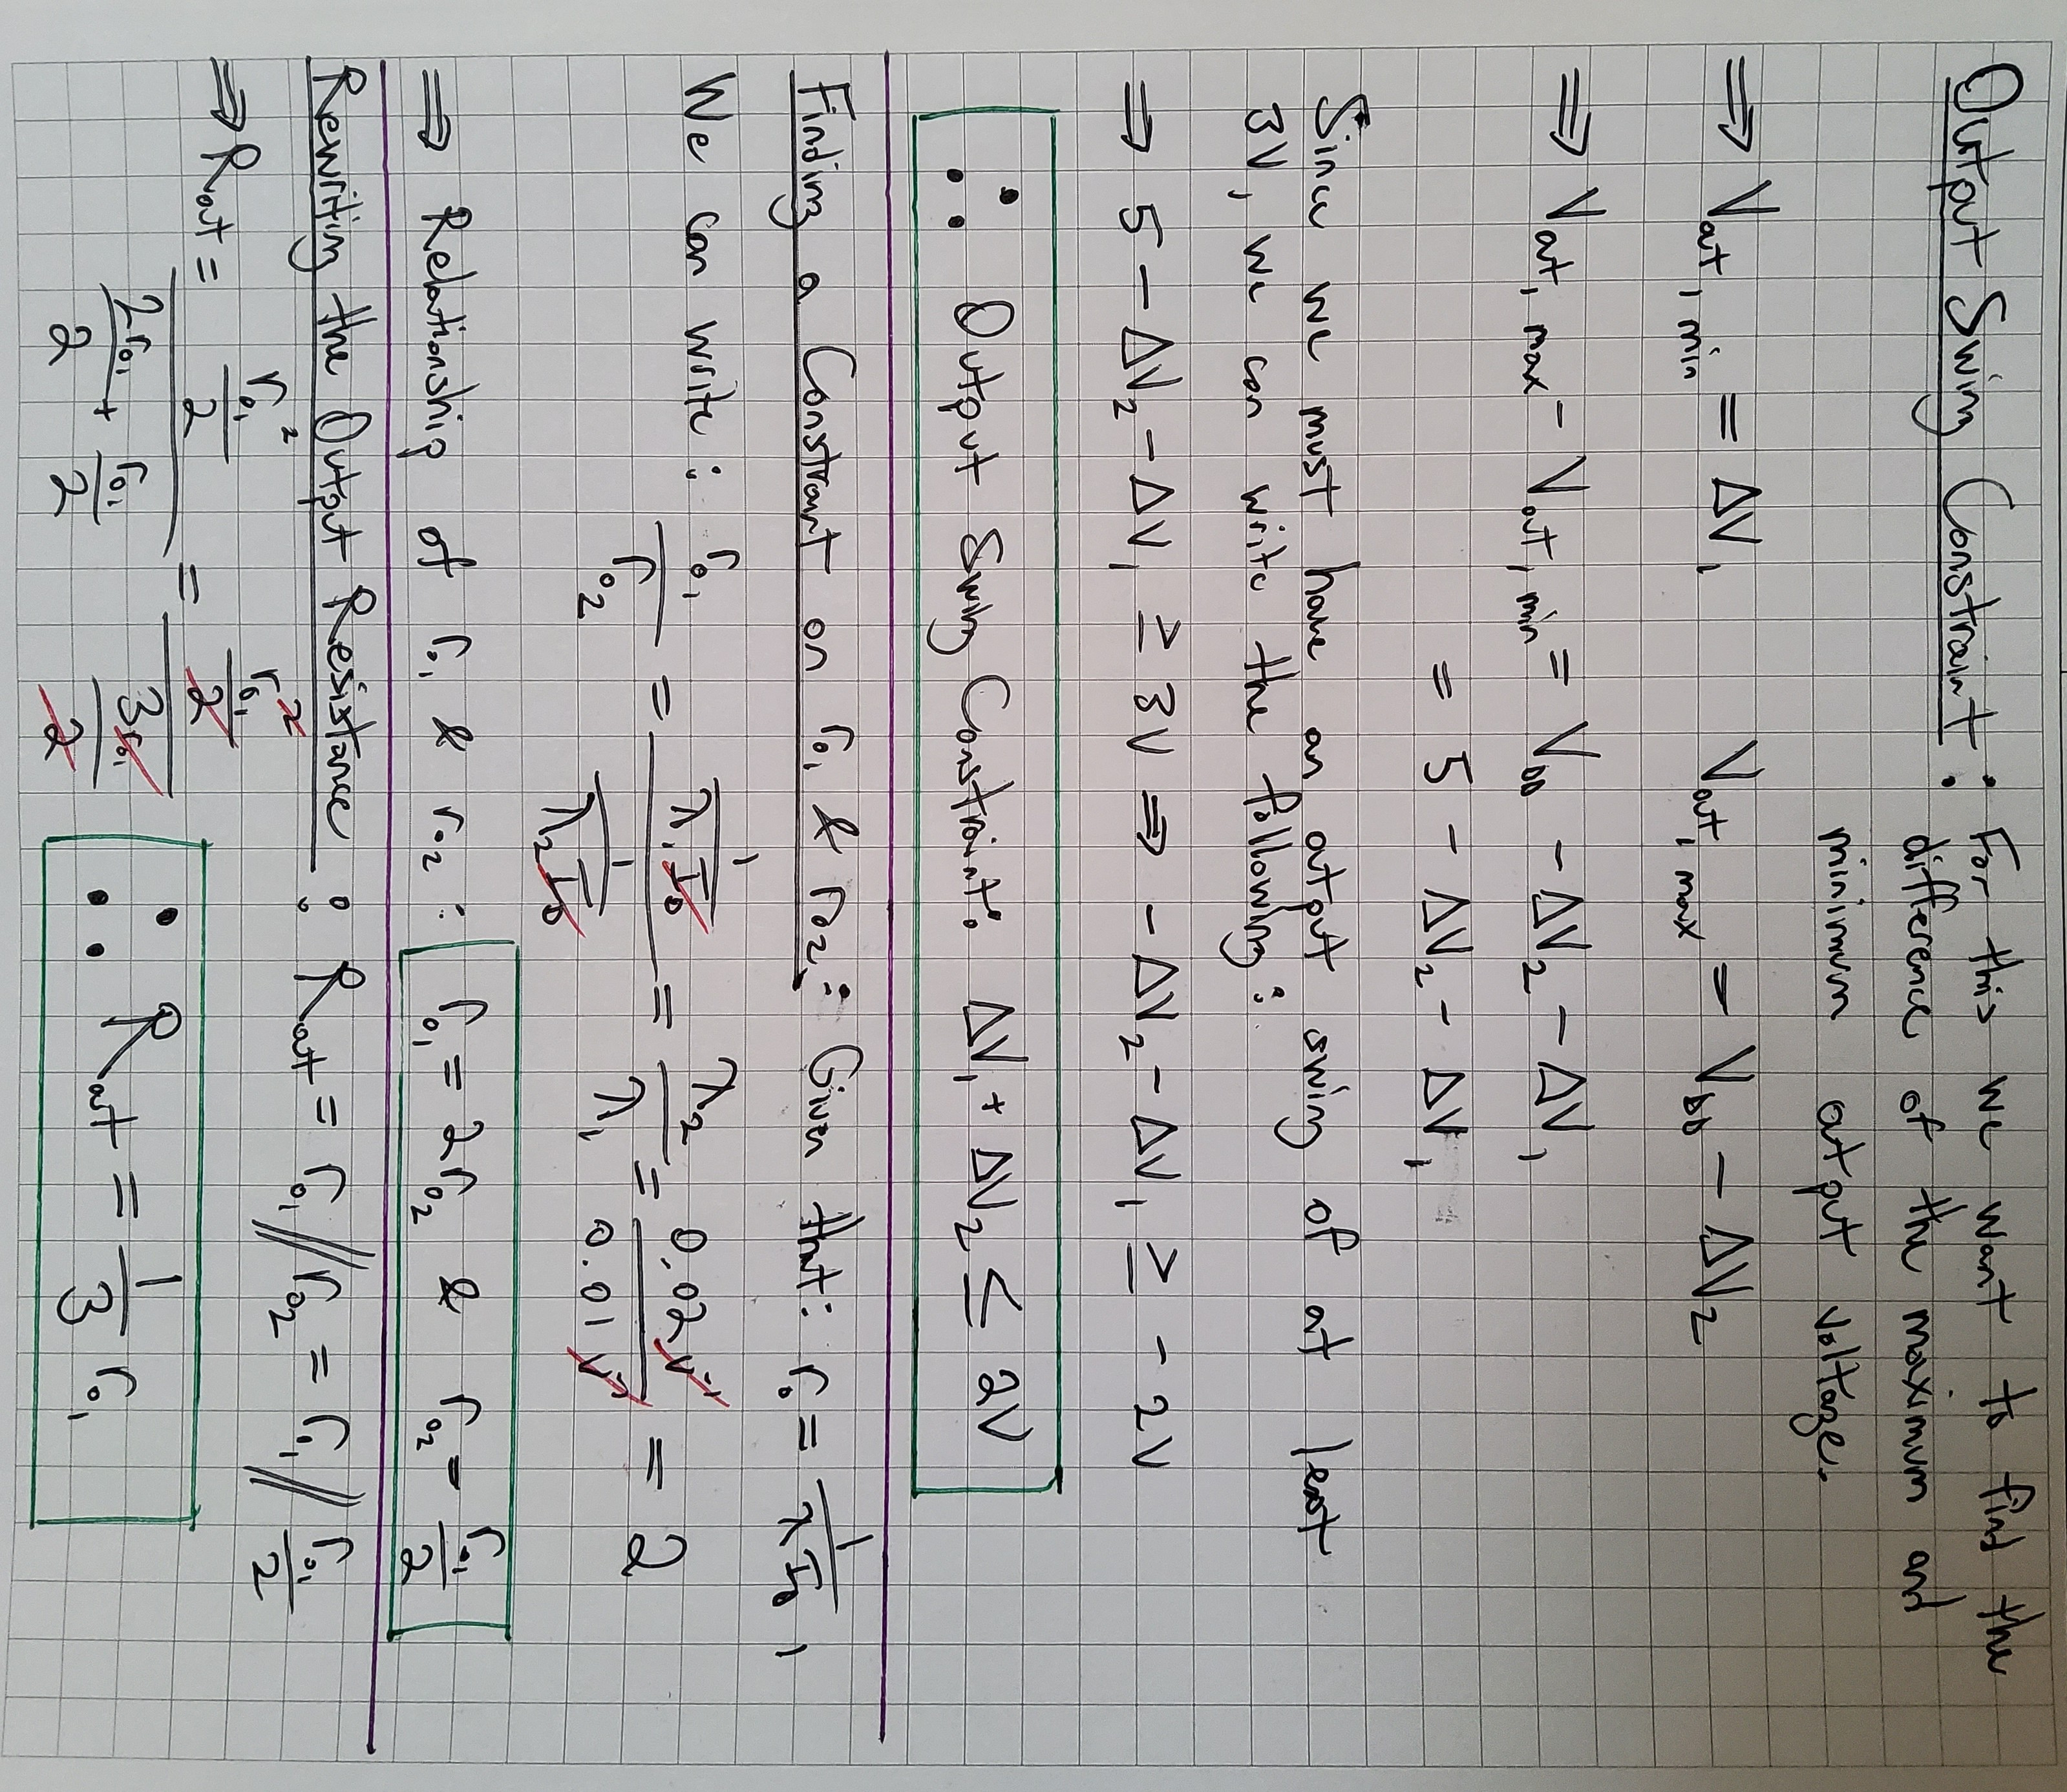
\includegraphics[scale=0.165, angle=90, center]{p2a_3.jpg}\\
\newpage
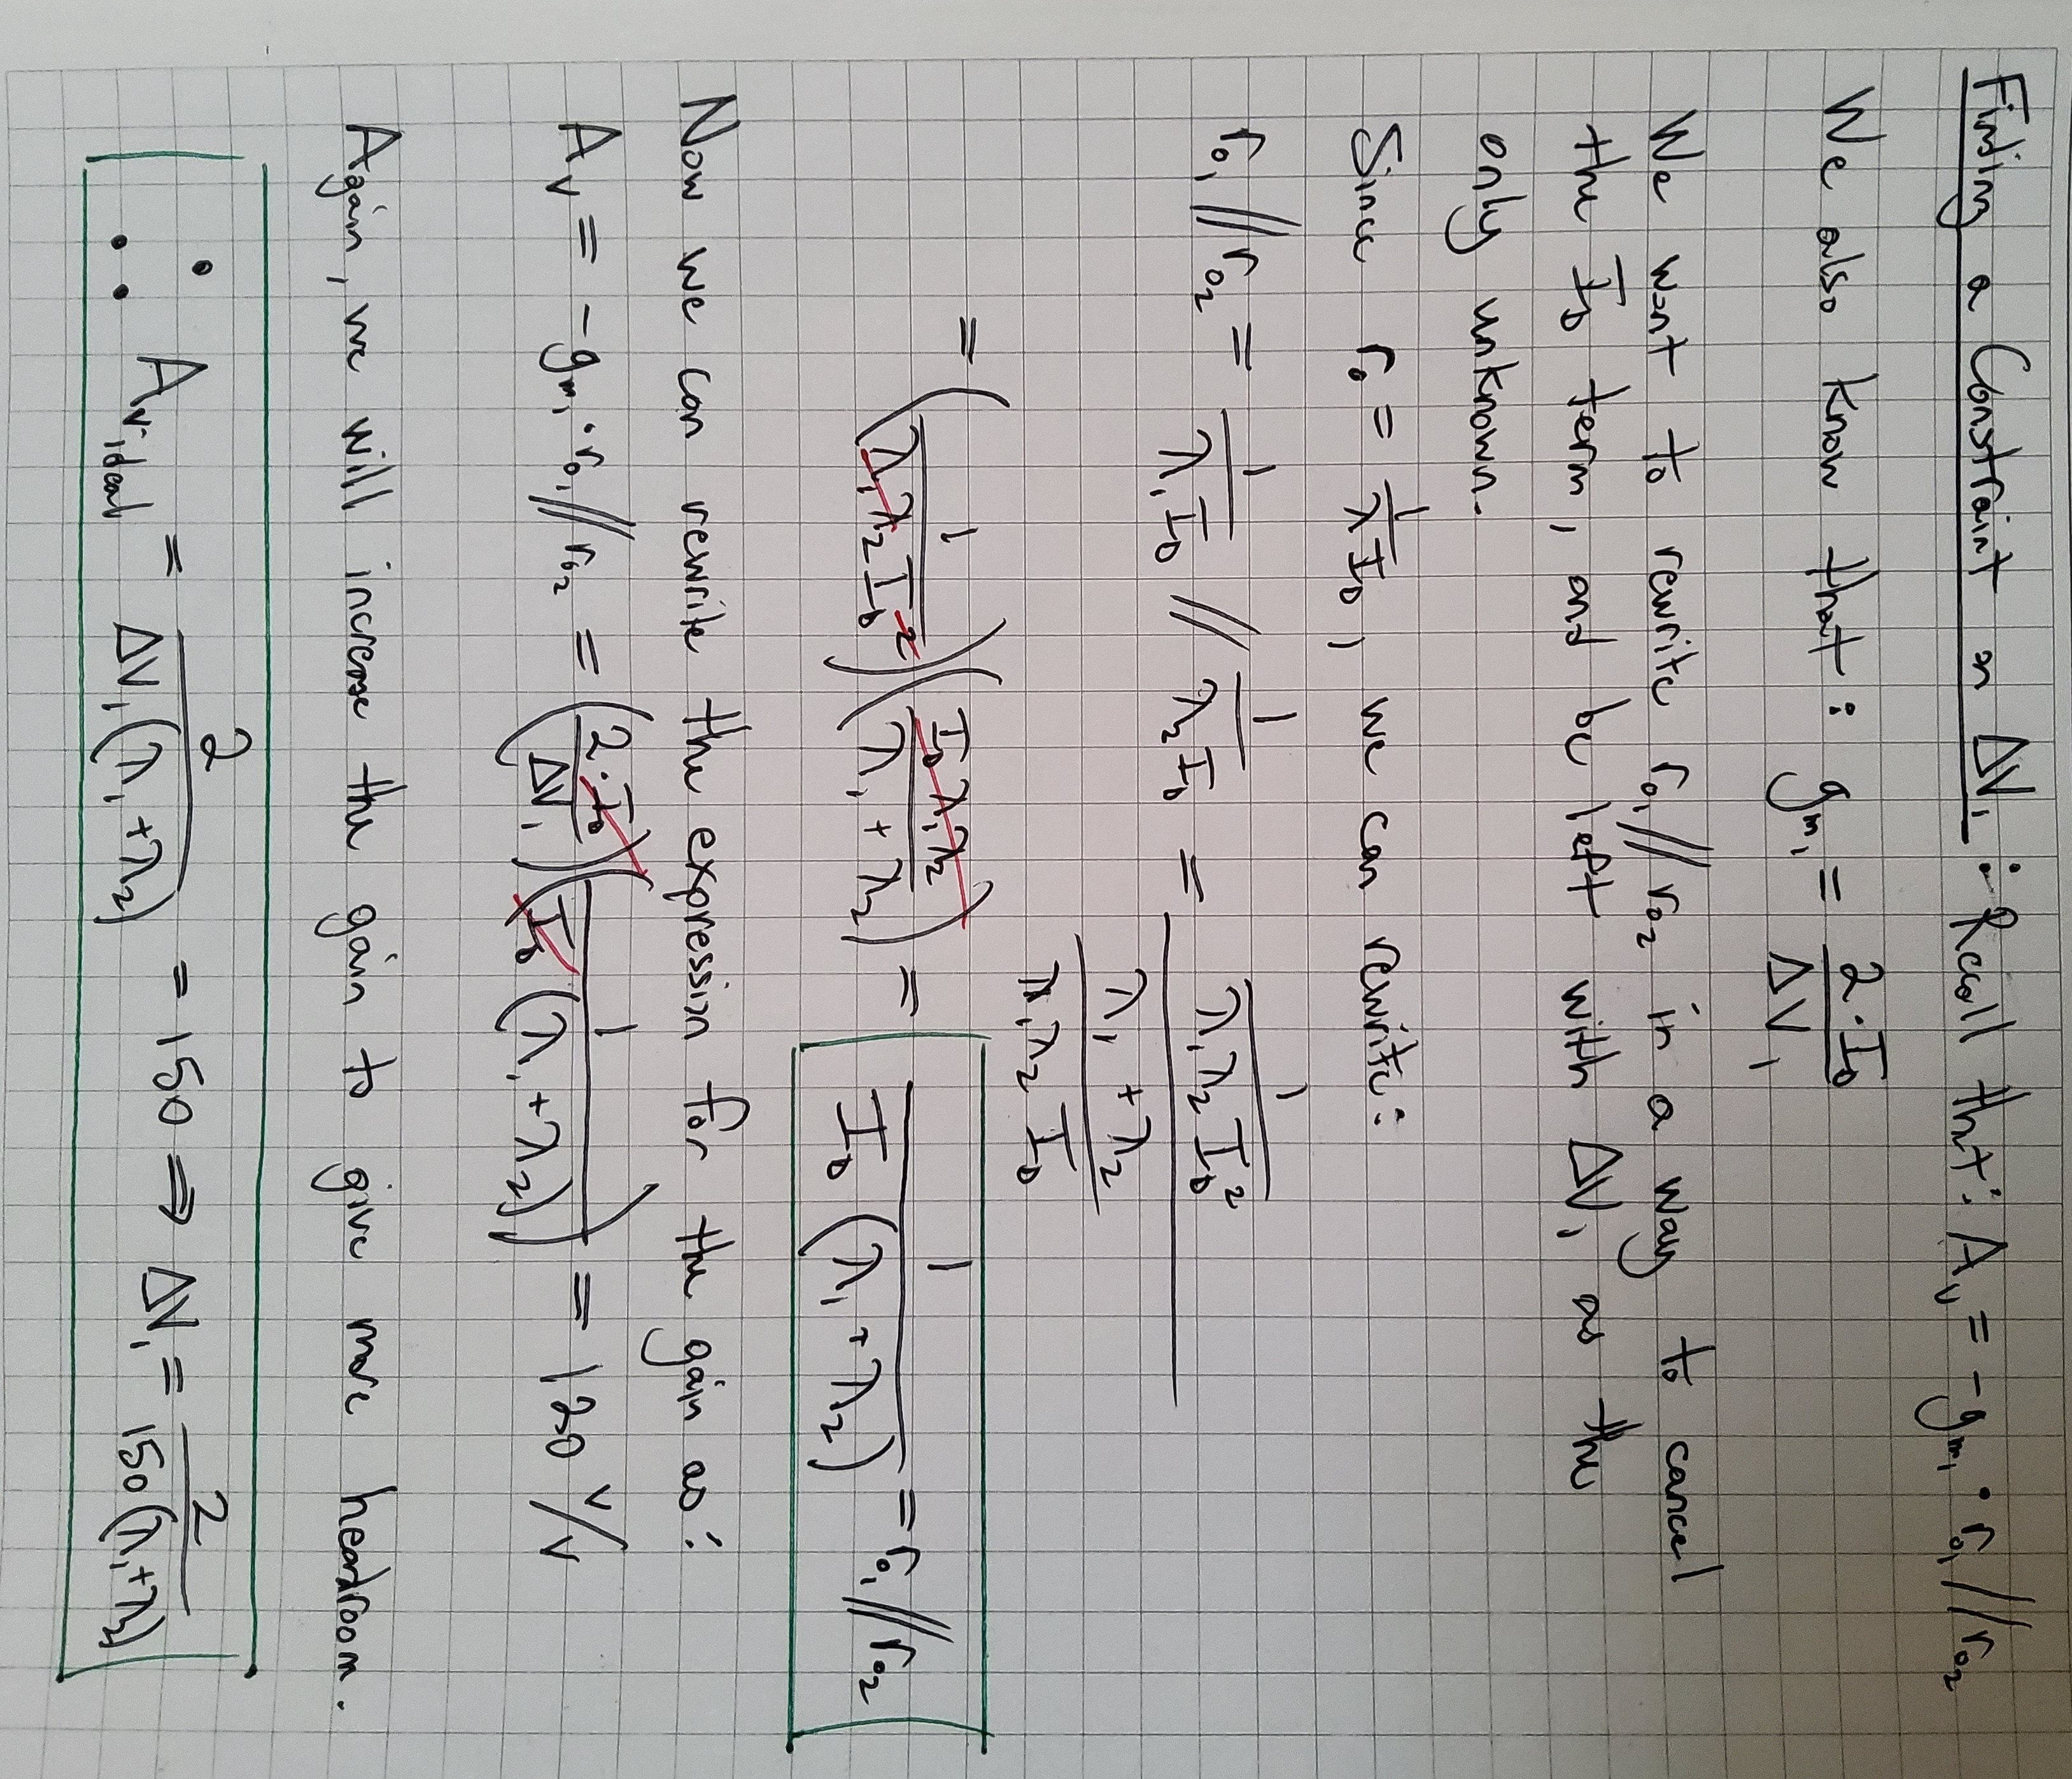
\includegraphics[scale=0.165, angle=90, center]{p2a_4.jpg}\\
\newpage
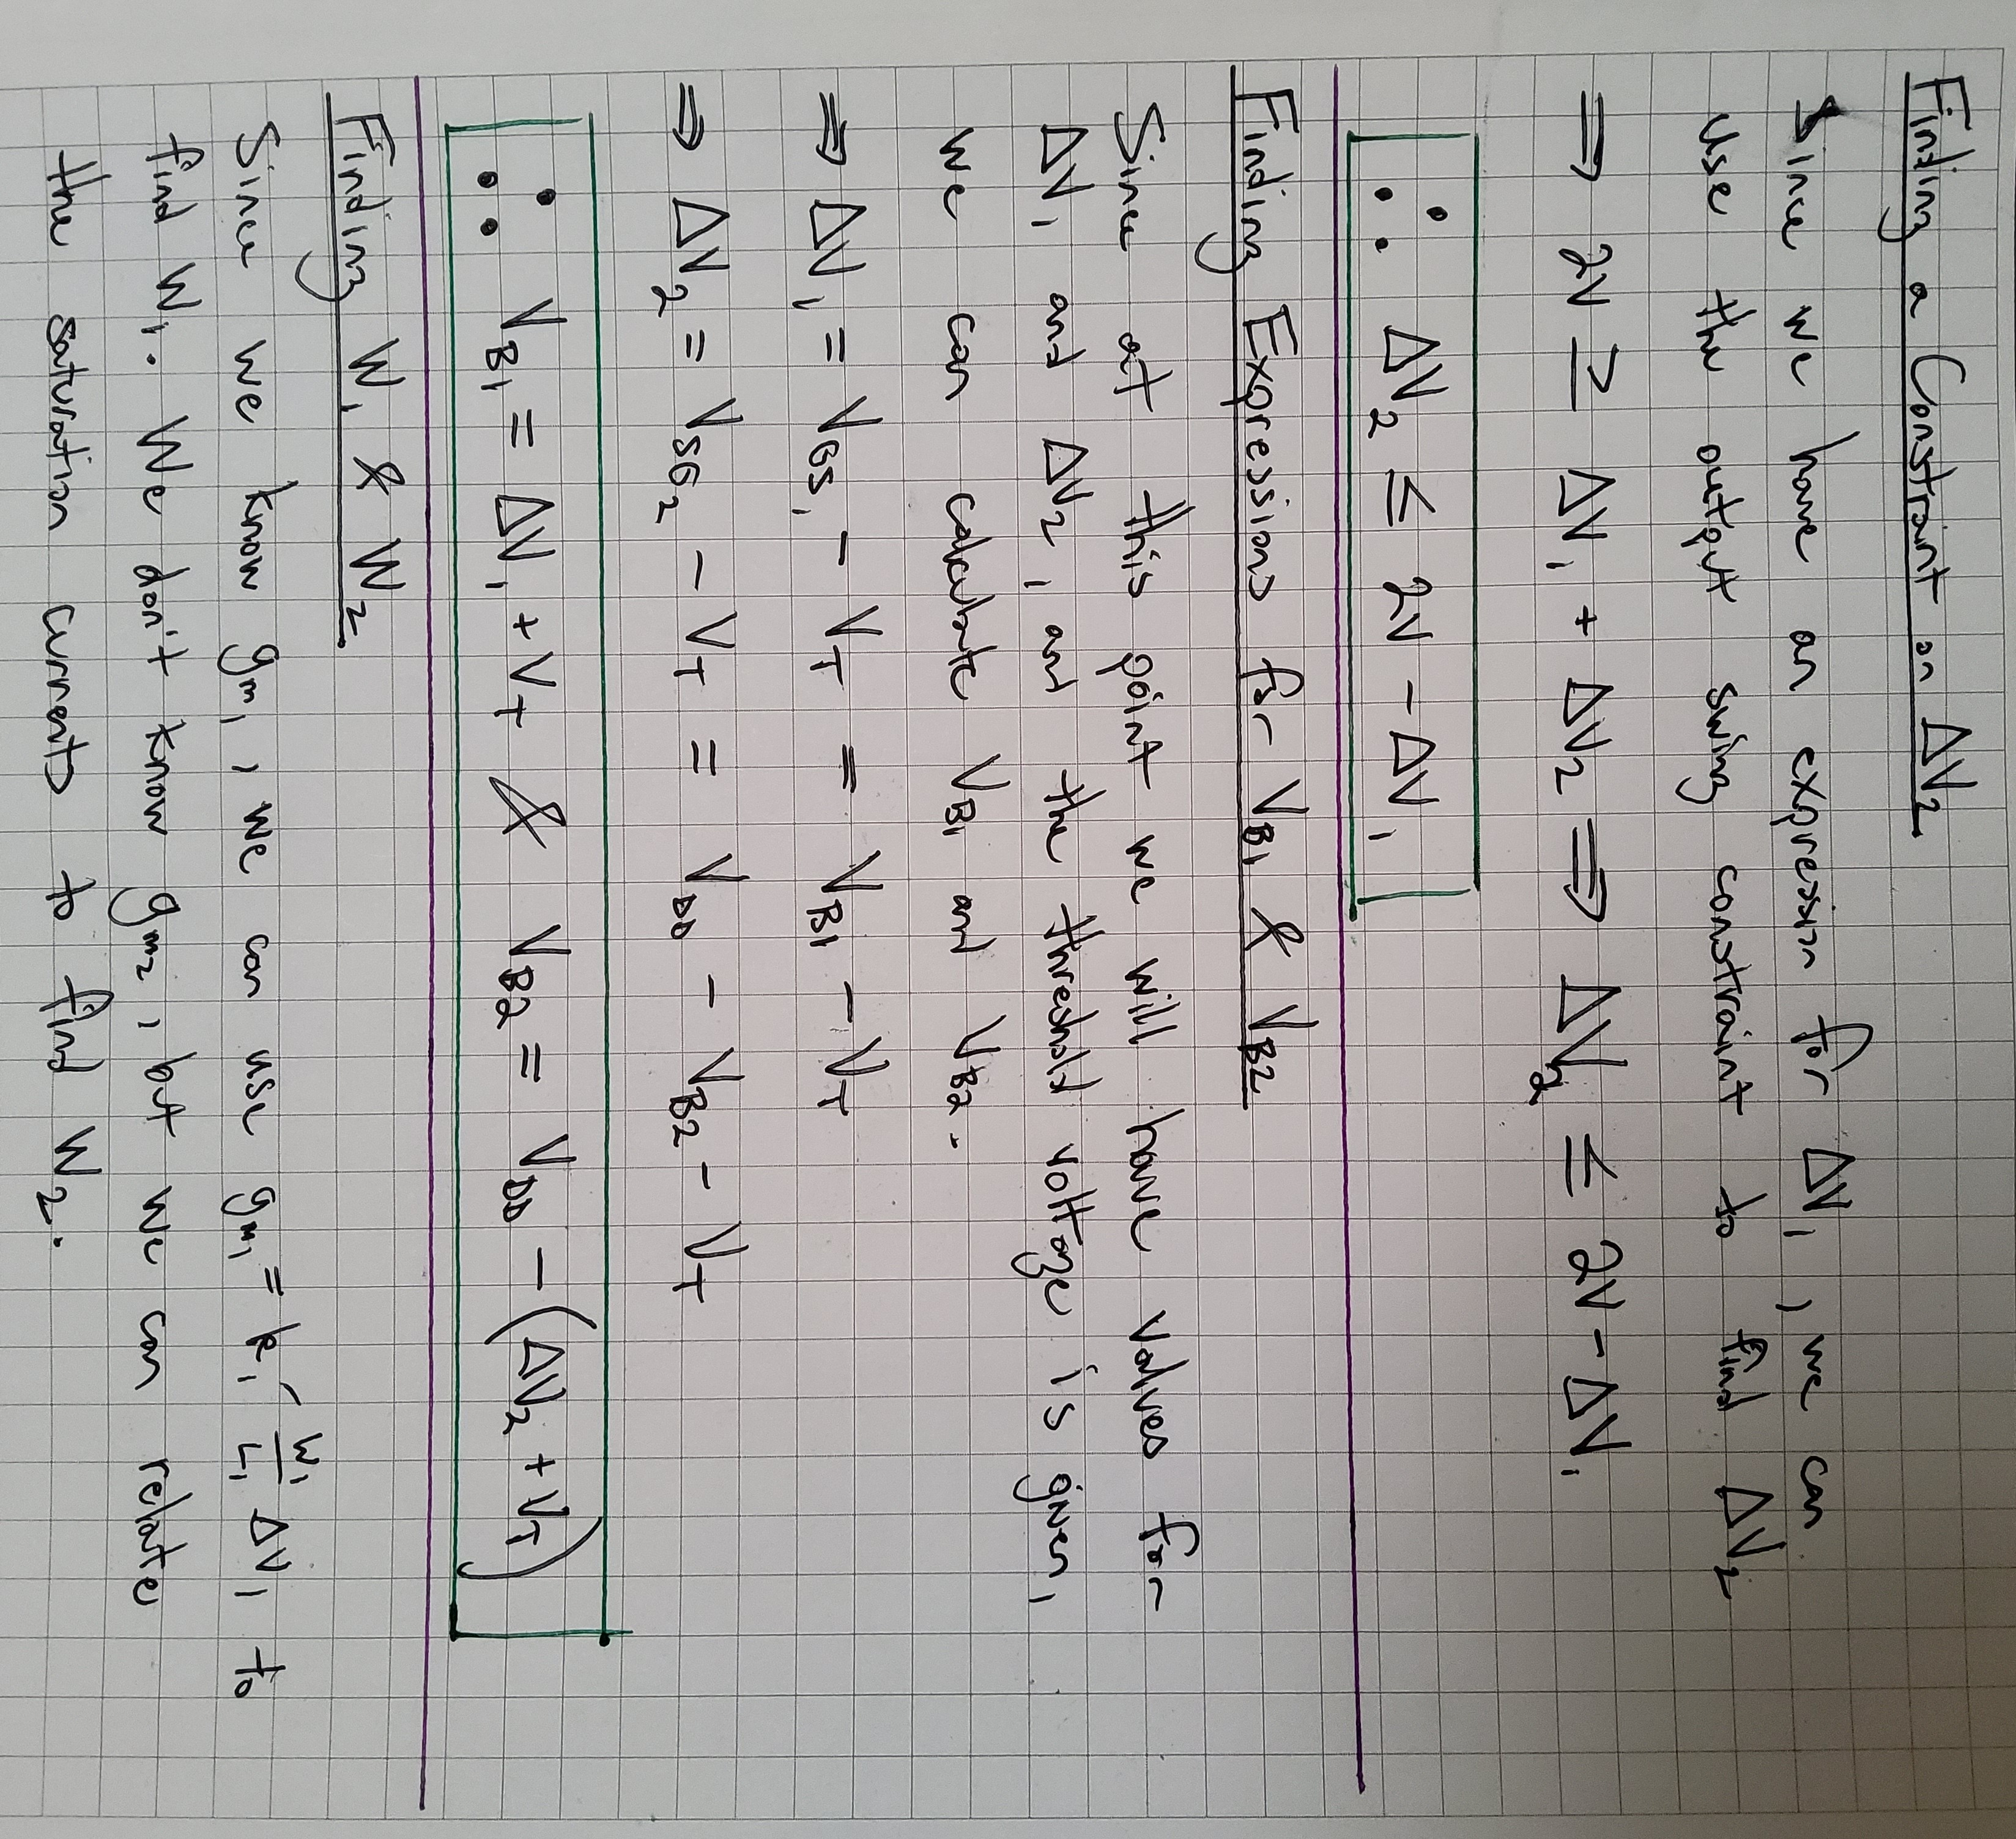
\includegraphics[scale=0.165, angle=90, center]{p2a_5.jpg}\\
\newpage
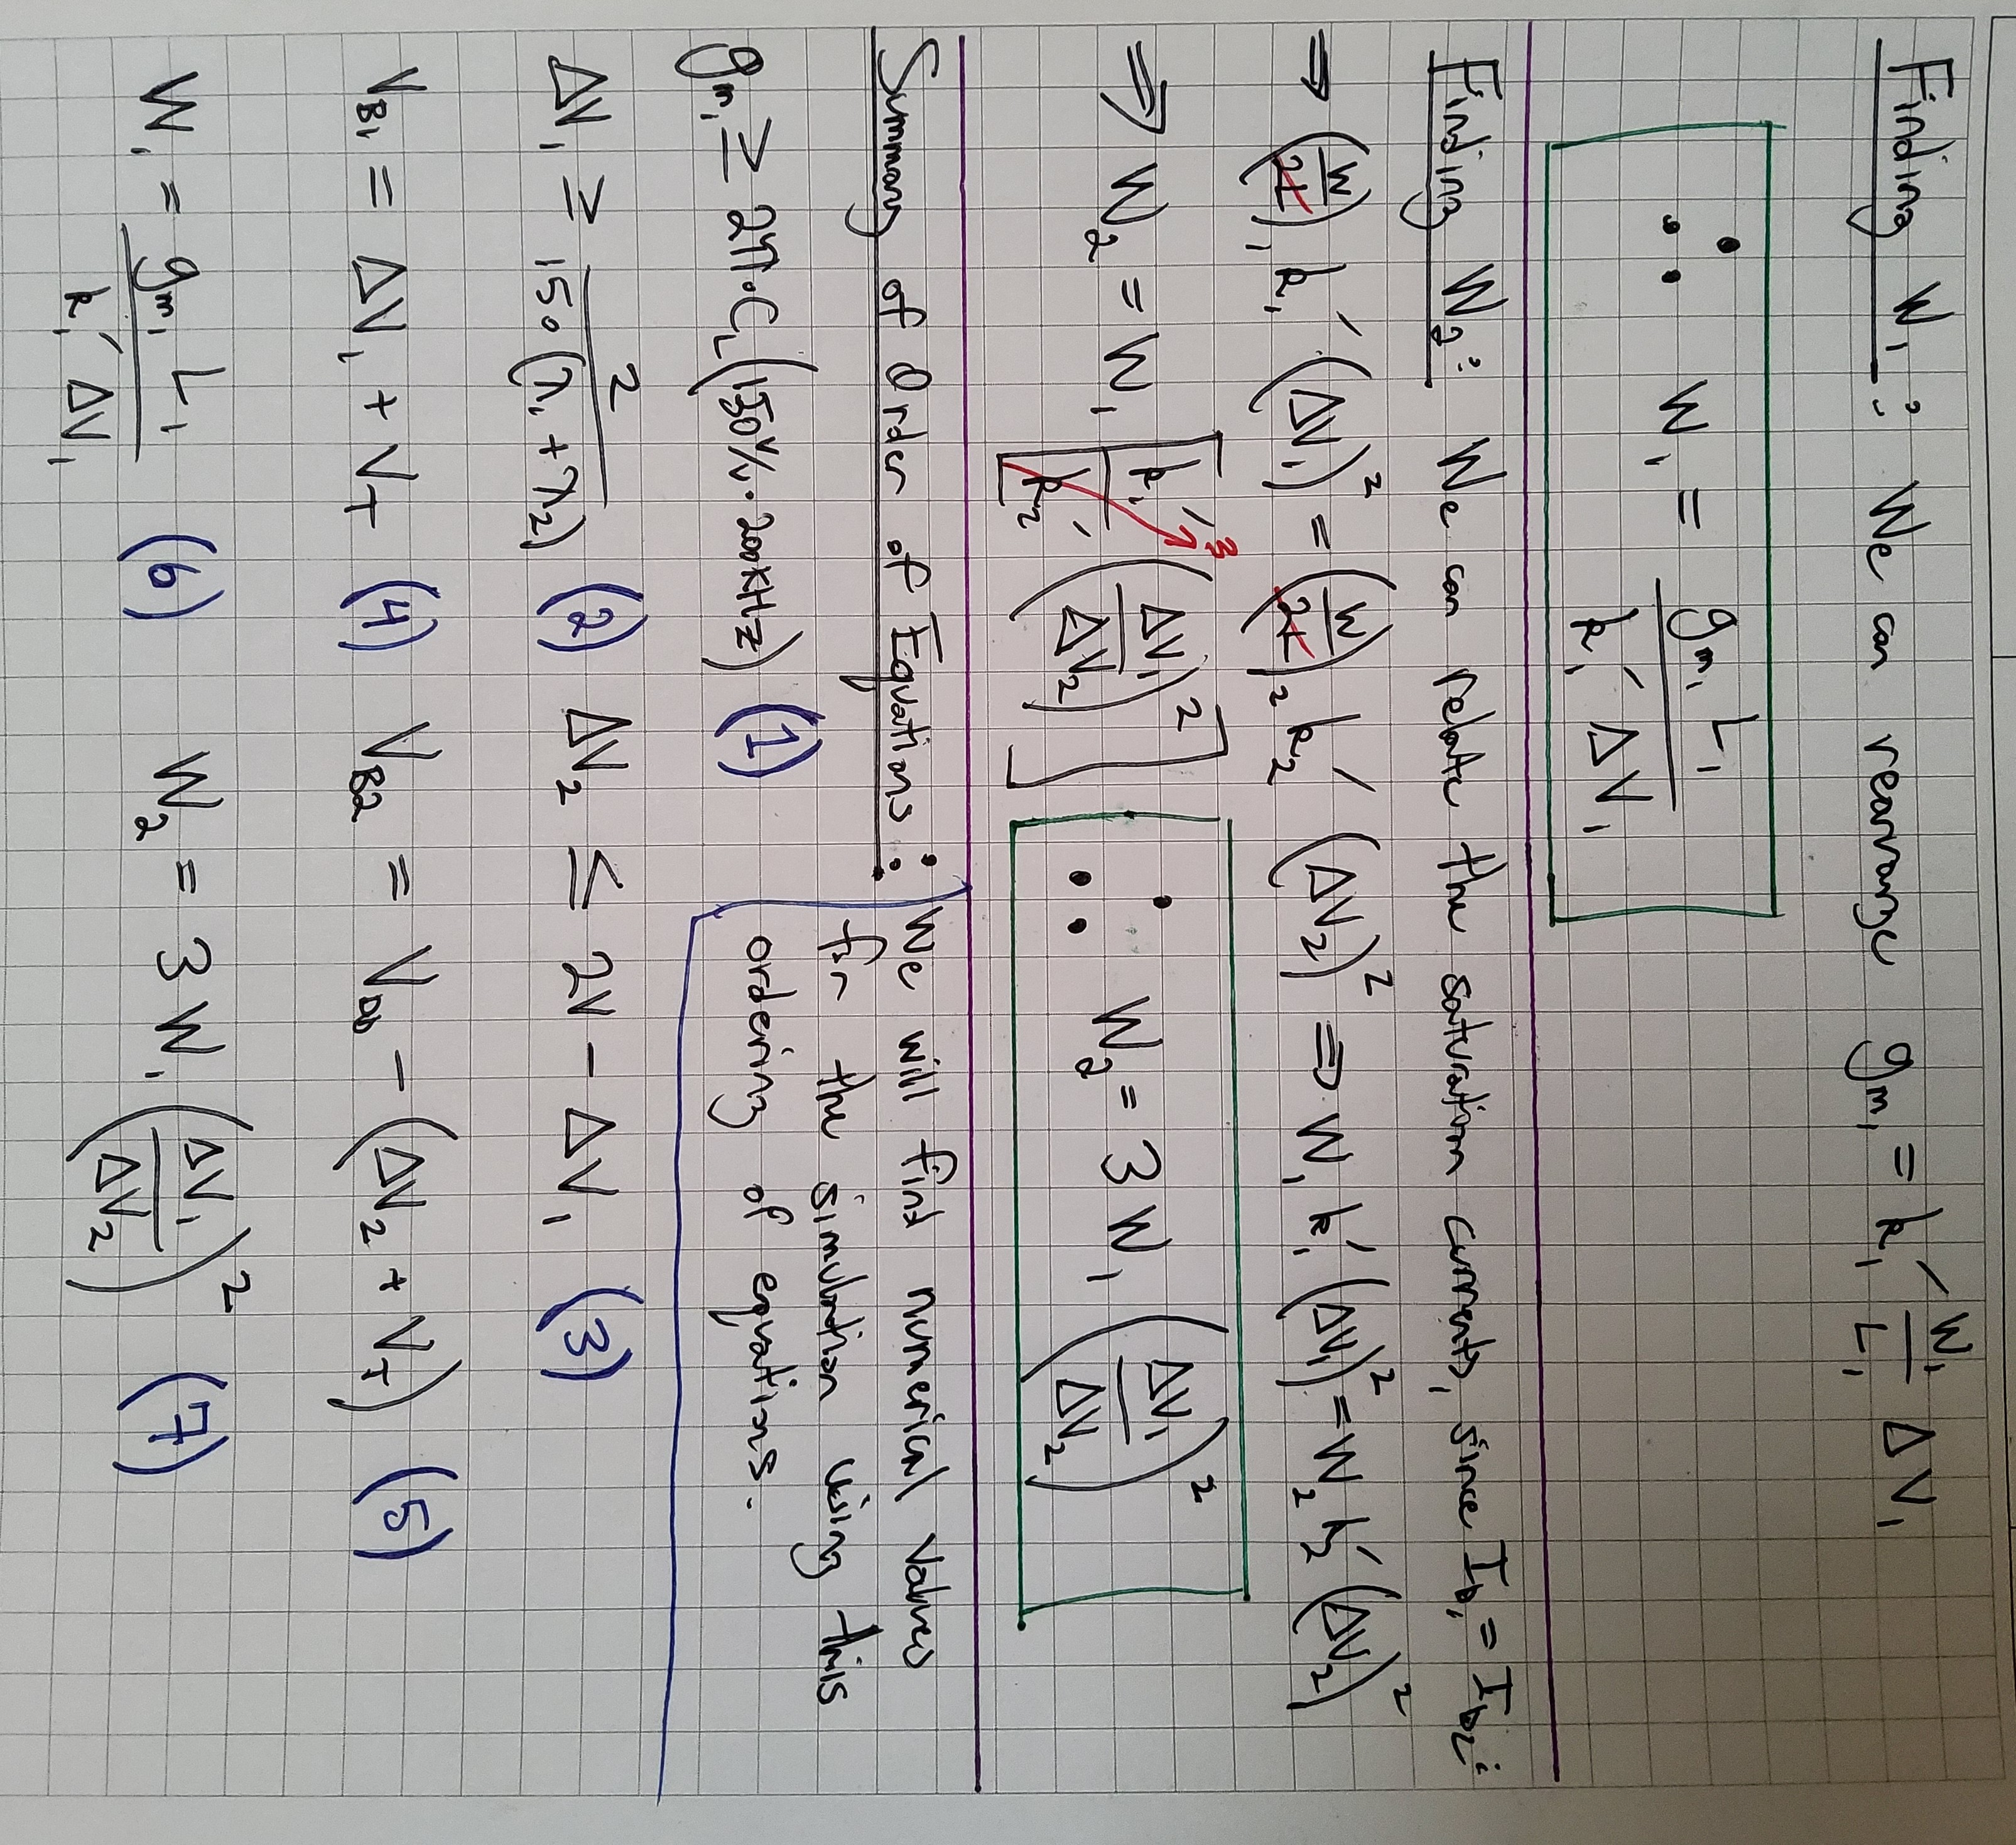
\includegraphics[scale=0.165, angle=90, center]{p2a_6.jpg}\\
\newpage
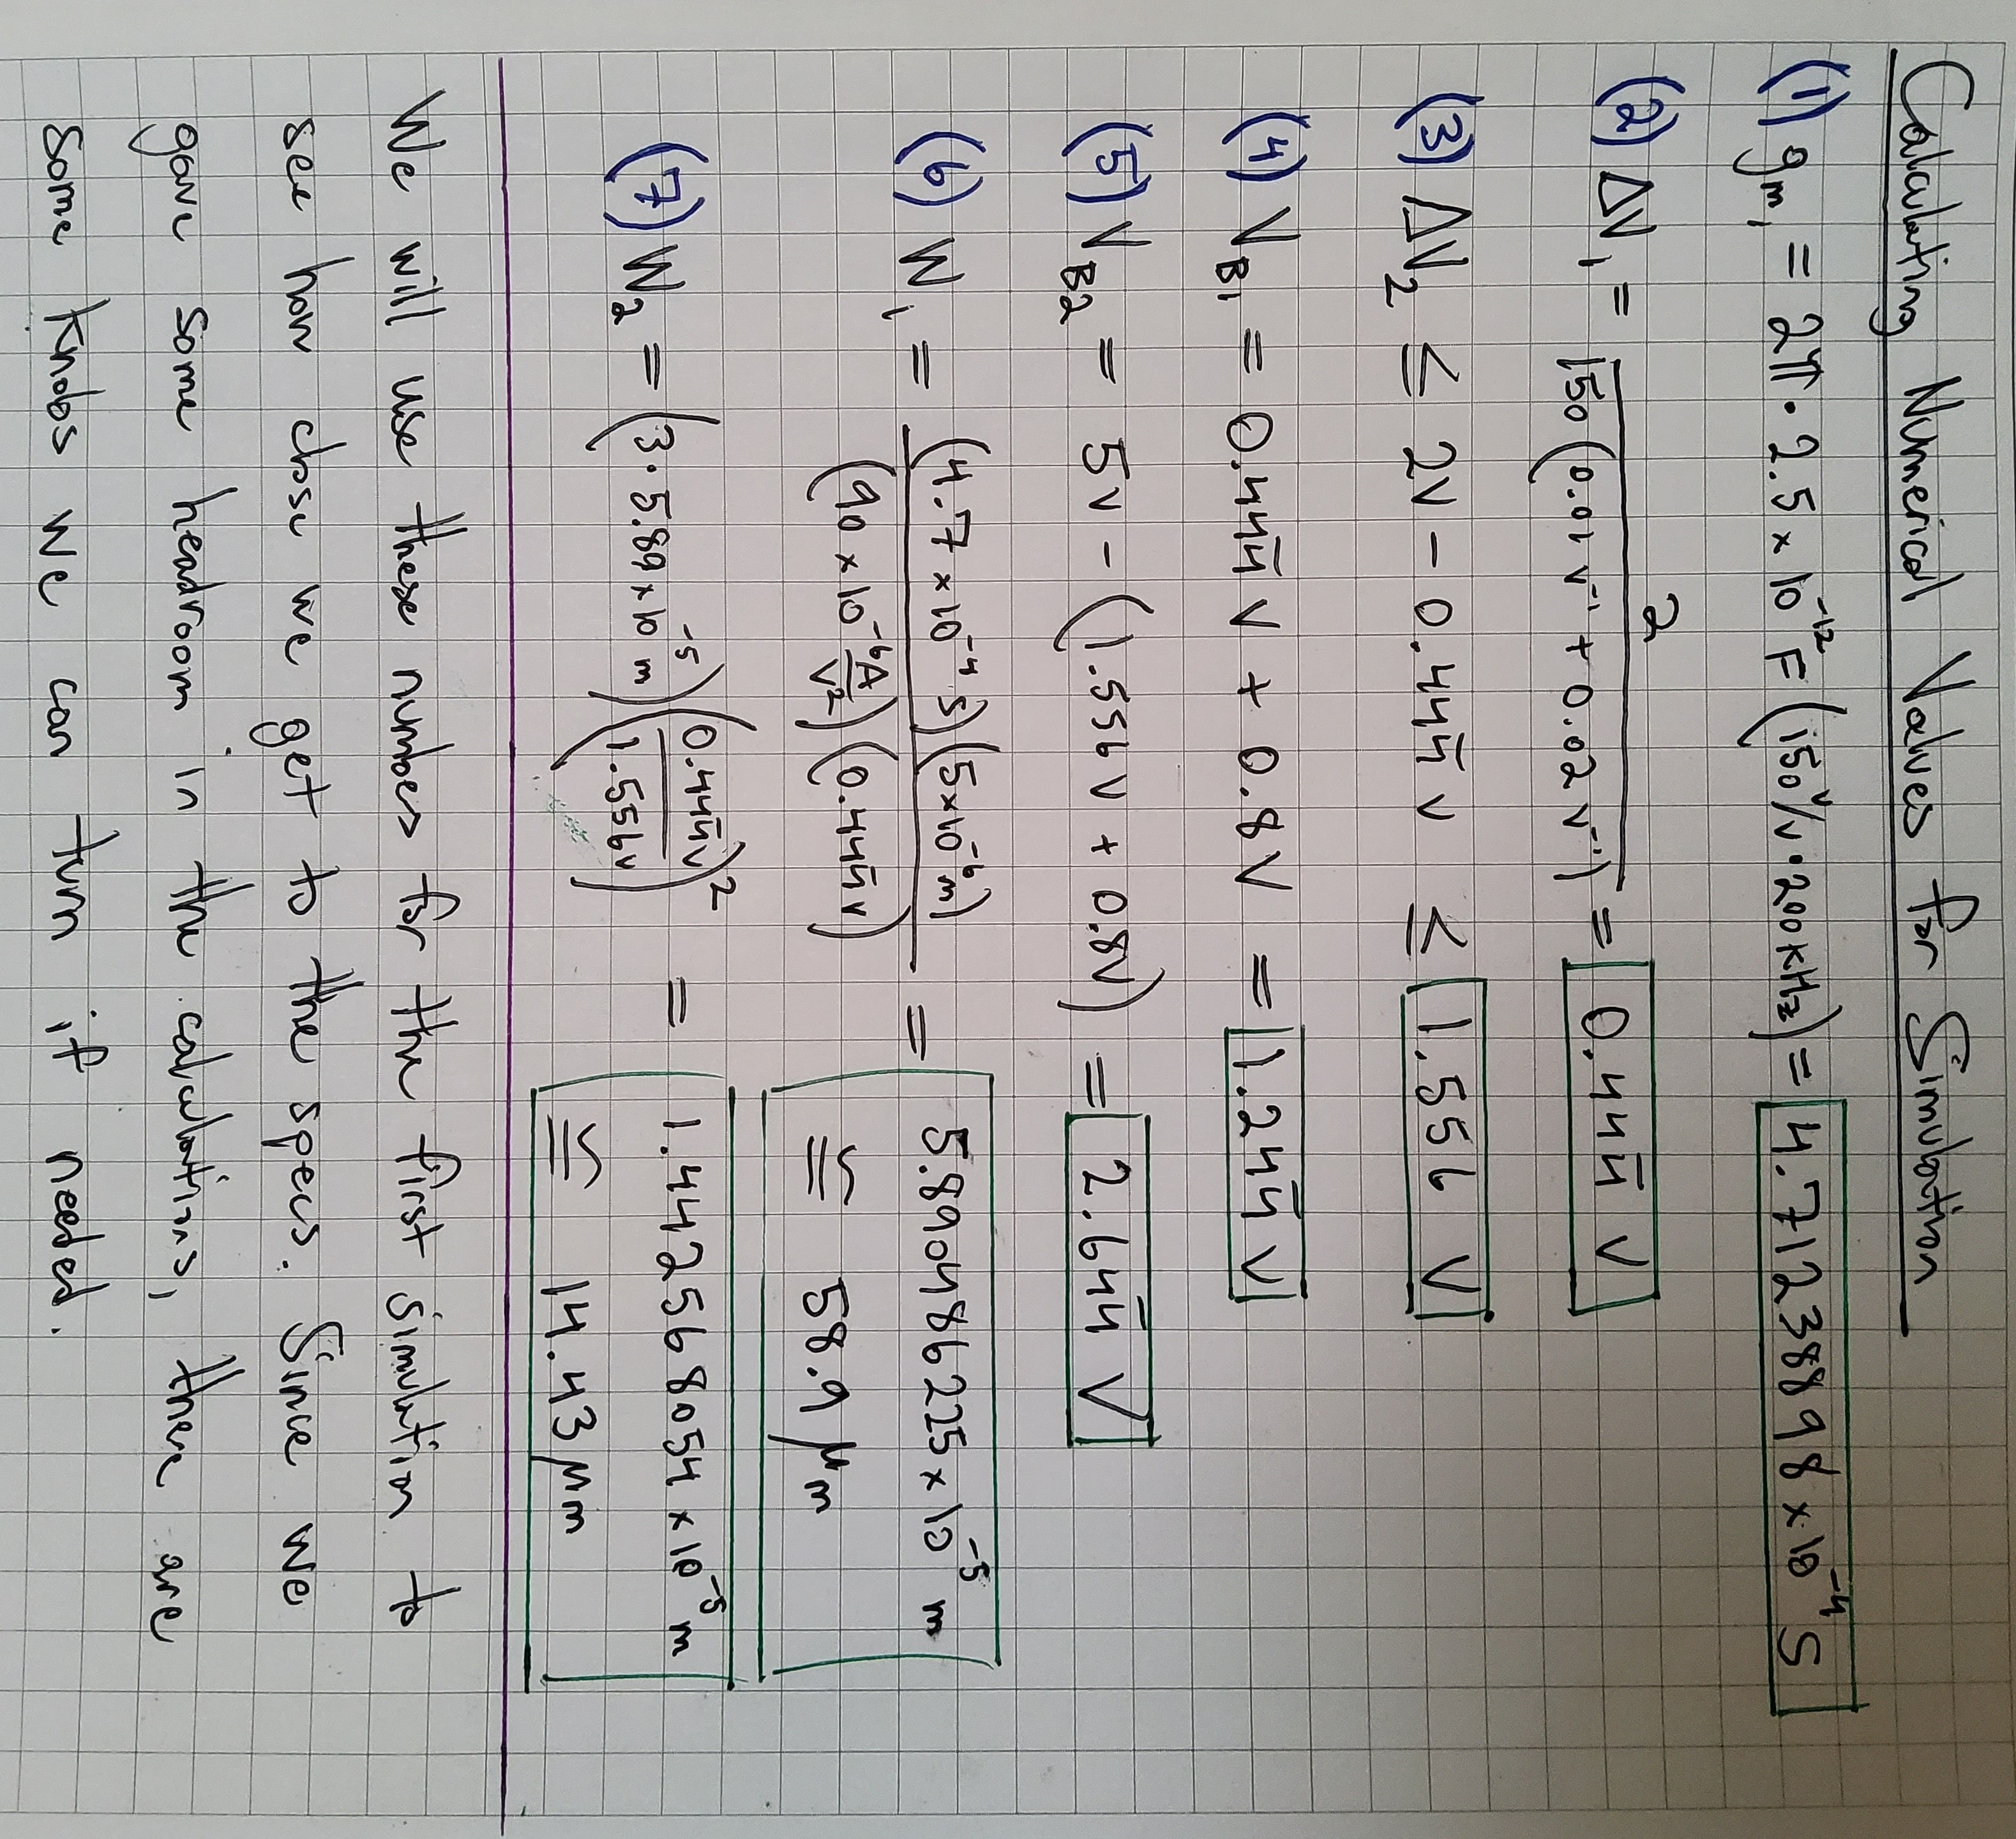
\includegraphics[scale=0.165, angle=90, center]{p2a_7.jpg}\\
\newpage
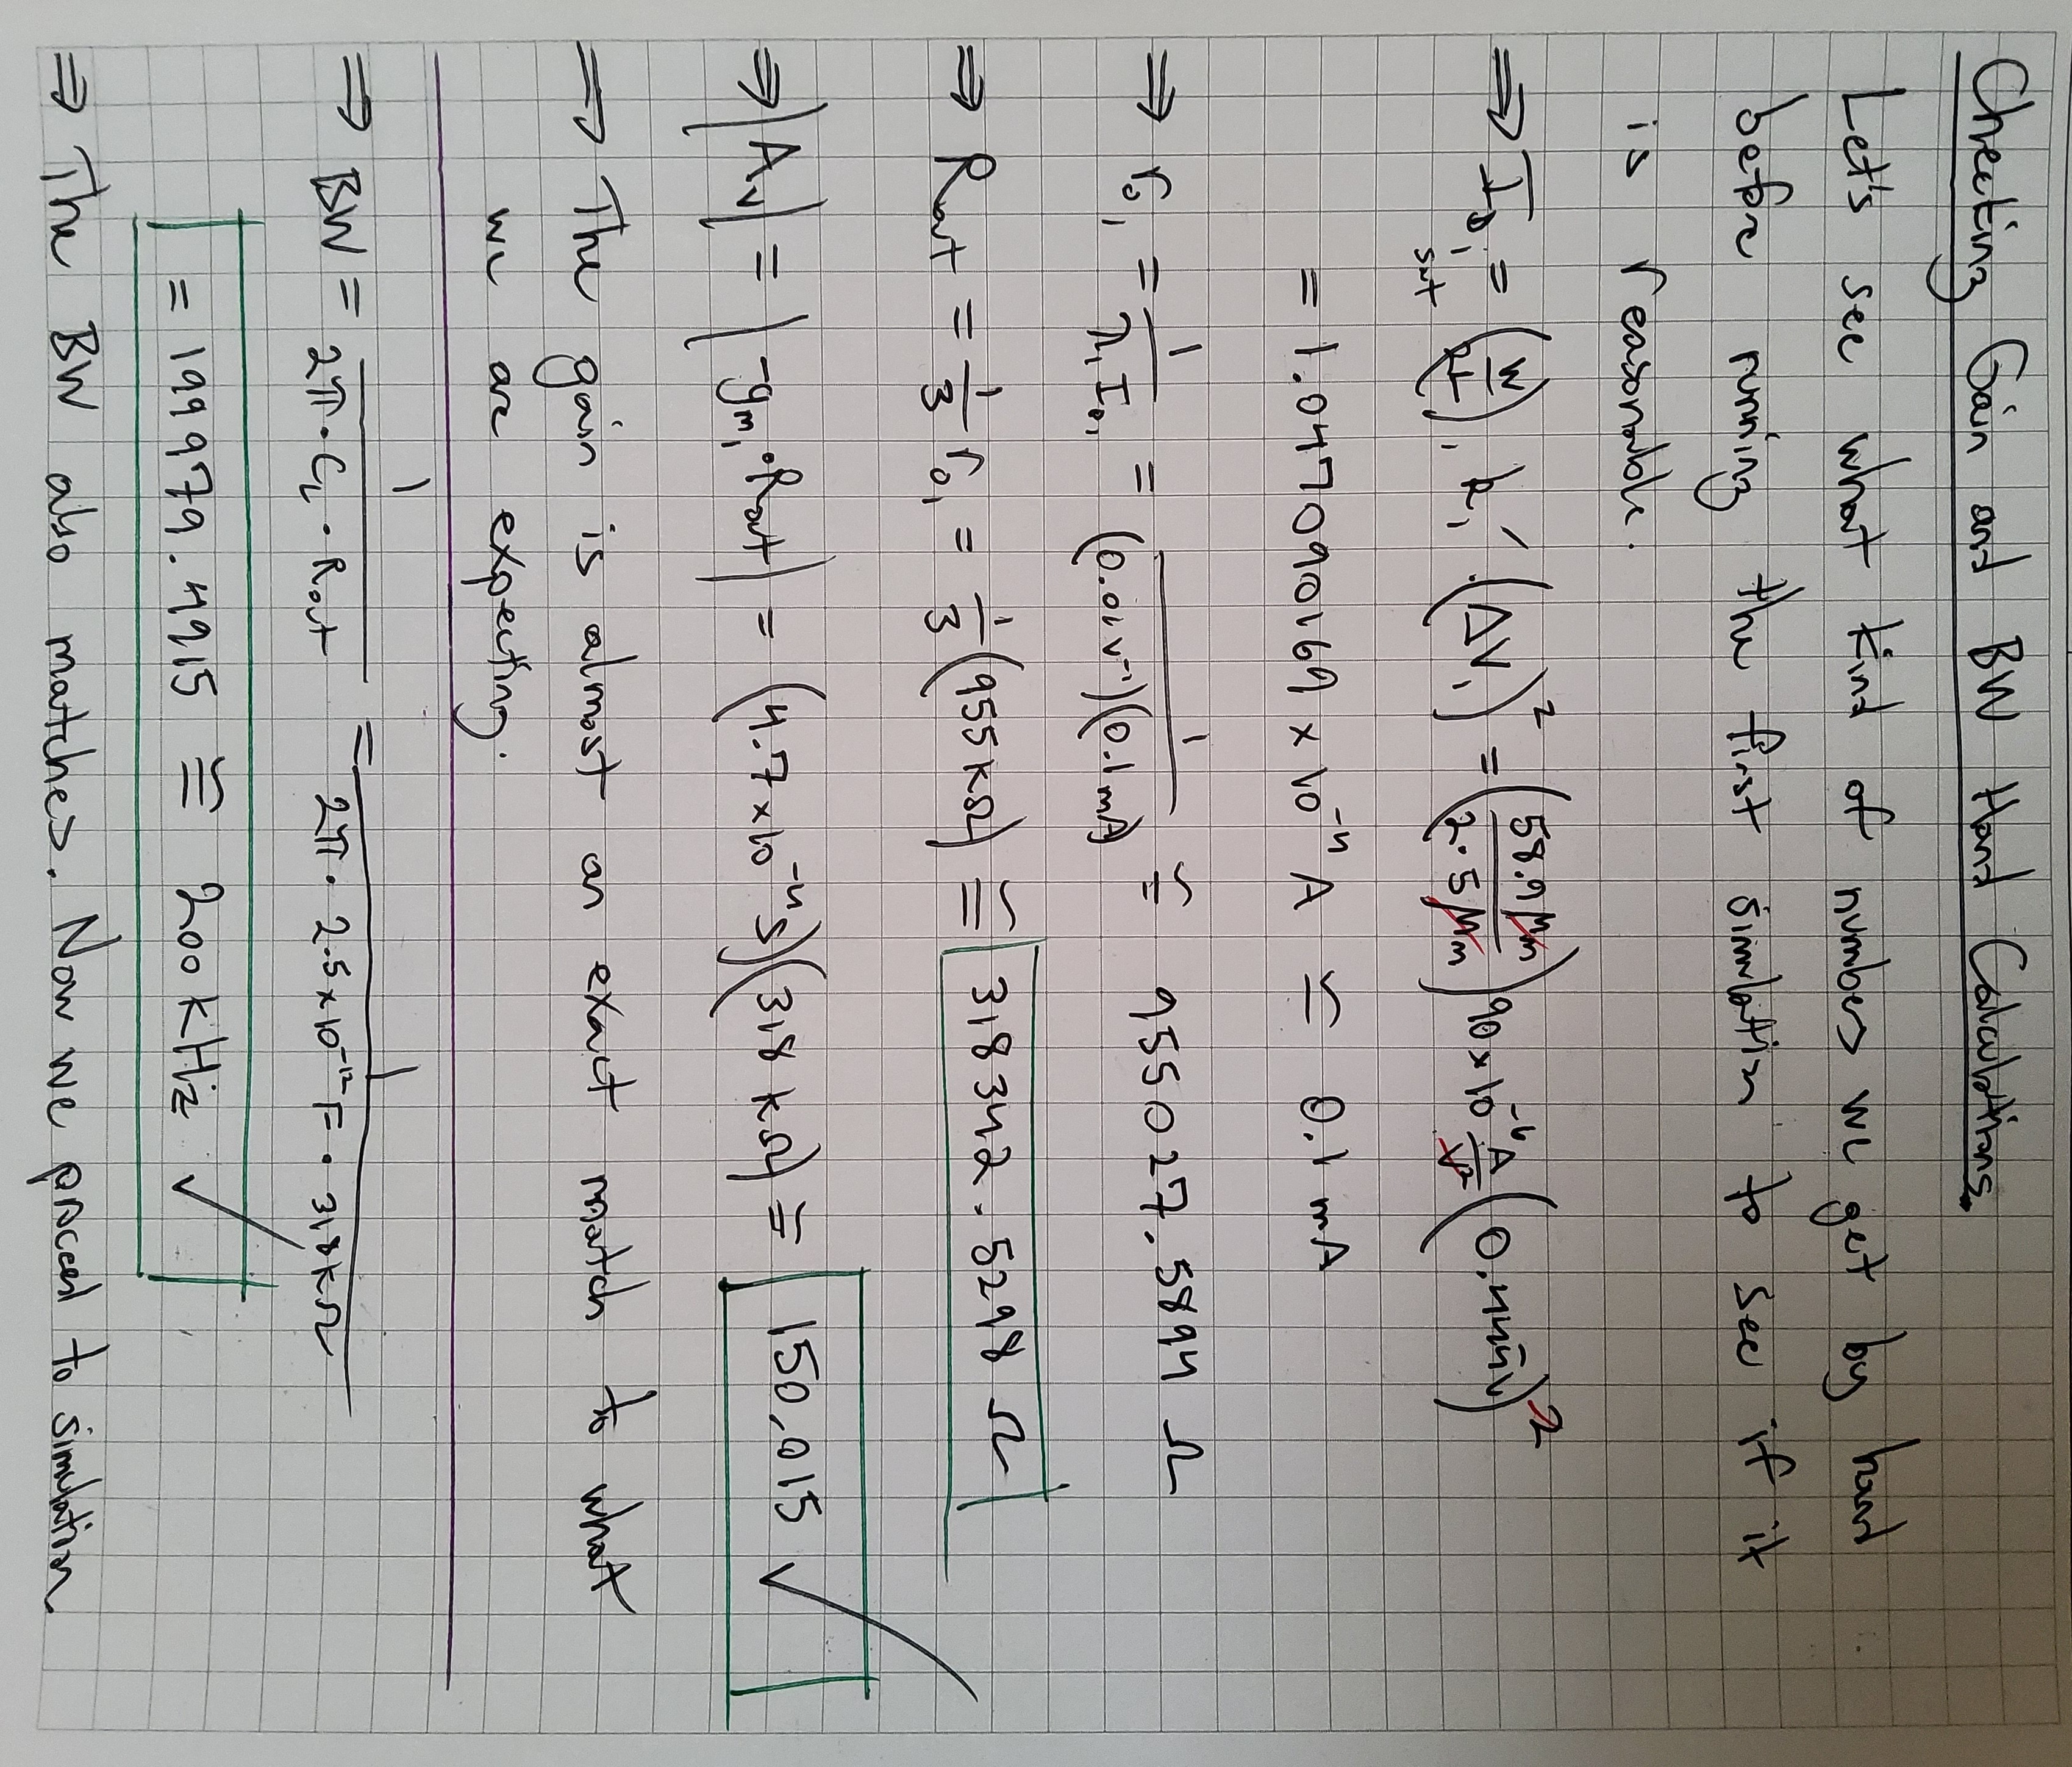
\includegraphics[scale=0.165, angle=90, center]{p2a_8.jpg}\\
\newpage
%%%%%%%%%%%%%%%%%%%%%%%%%%%%%%%%%%%%%%%%
%               SIMULATION             %
%%%%%%%%%%%%%%%%%%%%%%%%%%%%%%%%%%%%%%%%
\subsubsection{Simulation}
Below is the internal schematic of the amplifier used for simulation:\\[0.1cm]
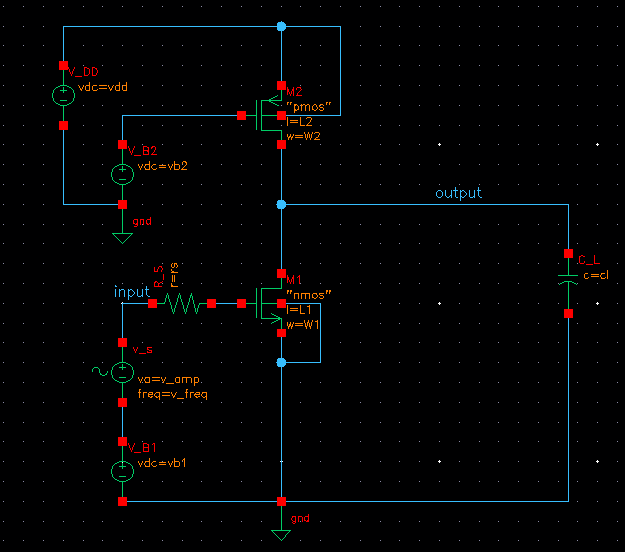
\includegraphics[scale=0.55, center]{c_internal.png}\\[0.25cm]
Below is the gain and bandwidth using our hand calculated numbers:\\[0.1cm]
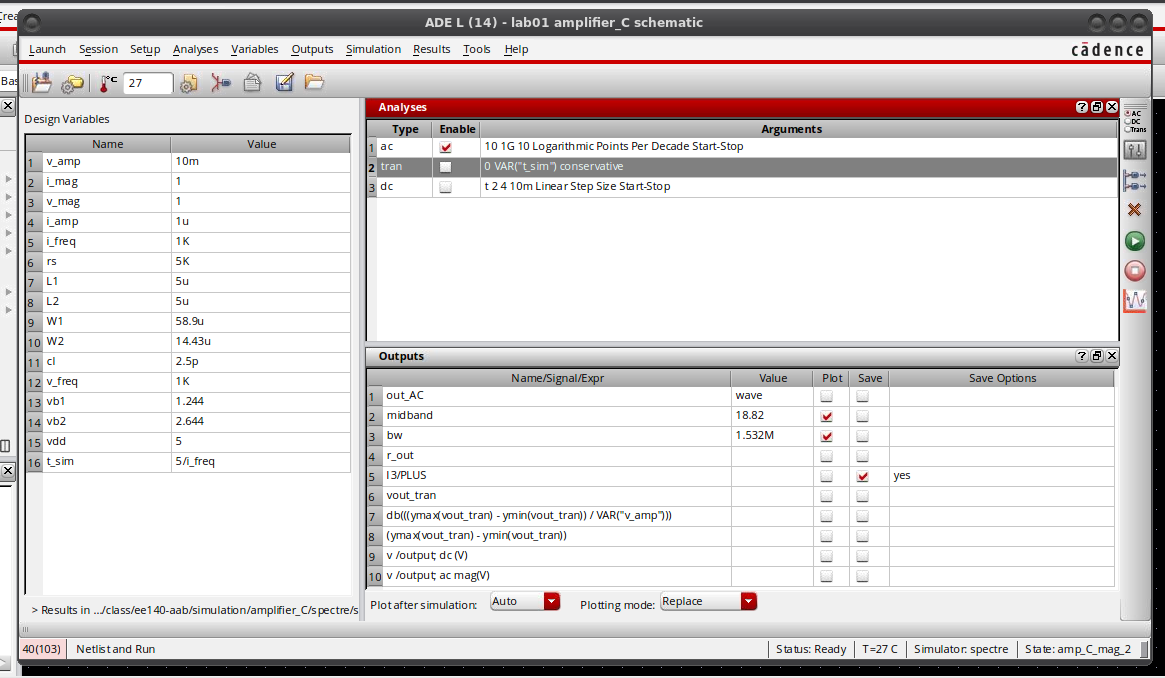
\includegraphics[scale=0.4, center]{c_gain_bw_init.png}
\newpage\noindent
We see that the gain is quite low, and the BW is quite large.  I decided to observe the DC voltages, because I want the output voltage to be at mid-rail for optimum performance, which is $V_{DD} / 2 = 2.5\,V$.  Below is a screenshot of the current node voltages:\\[0.1cm]
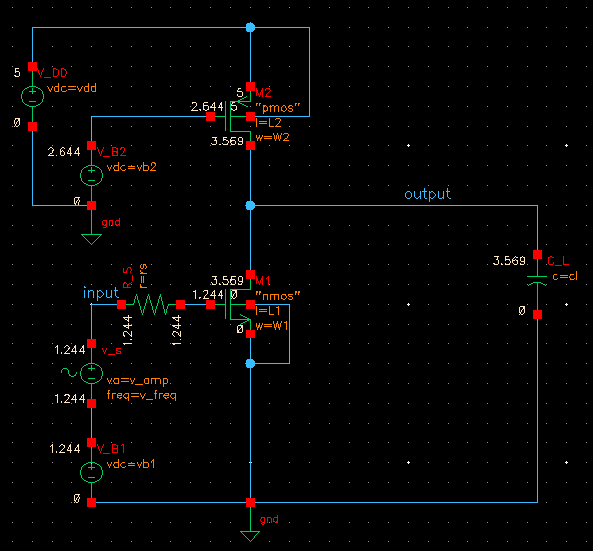
\includegraphics[scale=0.55, center]{c_dc_voltage.png}\\[0.25cm]
Because of the high gain requirement, $V_{B2}$ must be precisely tuned to meet the requirements, and our hand calculations are not that precise.  So we will sweep $V_{B2}$ to find what voltage will satisfy $2.5\,V$ at the output.  Below is the result of the sweep.\\[0.1cm]
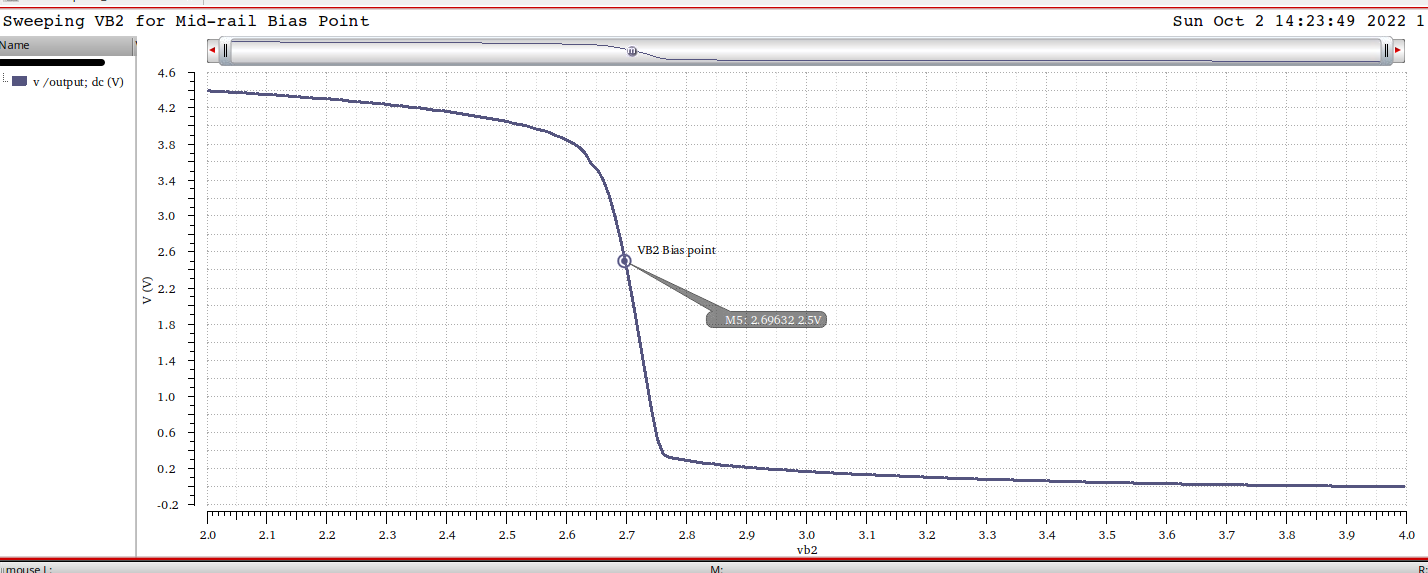
\includegraphics[scale=0.35, center]{c_dc_sweep.png}
\newpage\noindent
Now we run the simulation again with the new bias point of $2.696\,V$ for $V_{B2}$.  Below is a screenshot of the new results:\\[0.1cm]
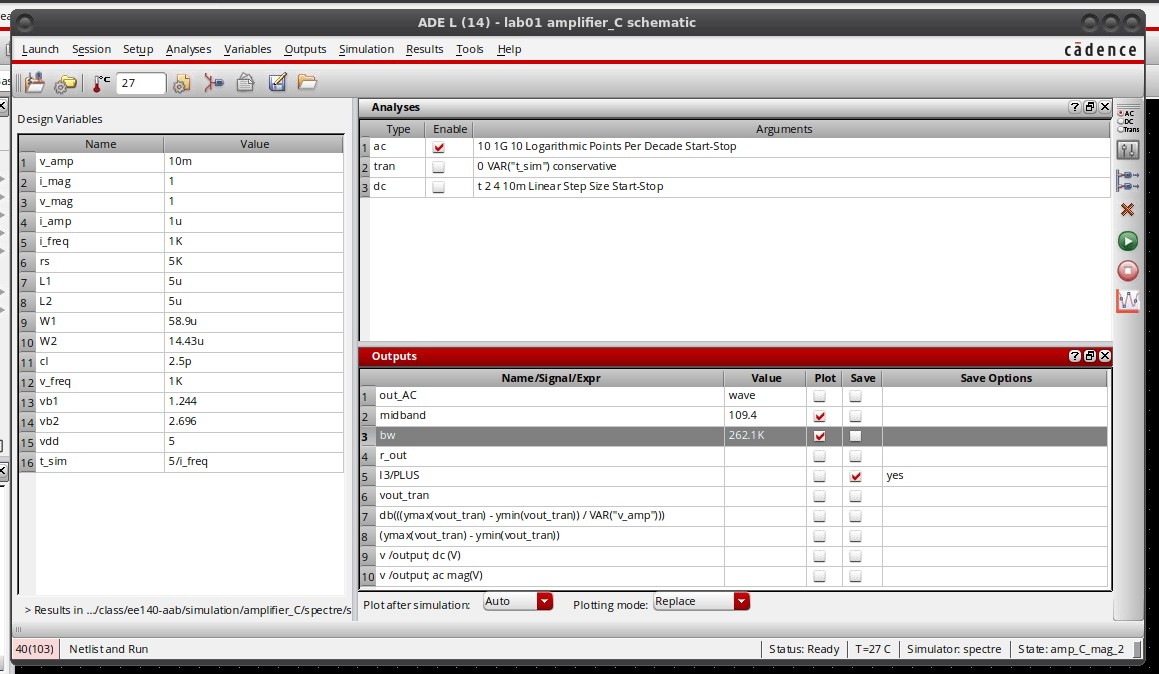
\includegraphics[scale=0.325, center]{c_gain_bw_new.png}\\[0.25cm]
The gain has come very close to our requirement of $120\,V/V$ with this adjustment, but it is not quite there.  The BW is also still quite large.

Since we had some headroom with the bias voltages, I will proceed by slightly decreasing $\Delta V_1$ in order to increase the gain, which should reduce the BW at the same time. We will have to use the formulas in the hand calculations to recalculate $\Delta V_2$, $V_{B1}$, $V_{B2}$, and the transistor widths.  For now we will leave $g_{m_1}$ alone, although there is also room to turn that dial if needed.  I will omit the calculations for brevity of this report, because they are the same process as already shown.

Below is the gain and BW with our new numbers after sweeping $V_{B2}$ to find the right operating point.\\[0.1cm]
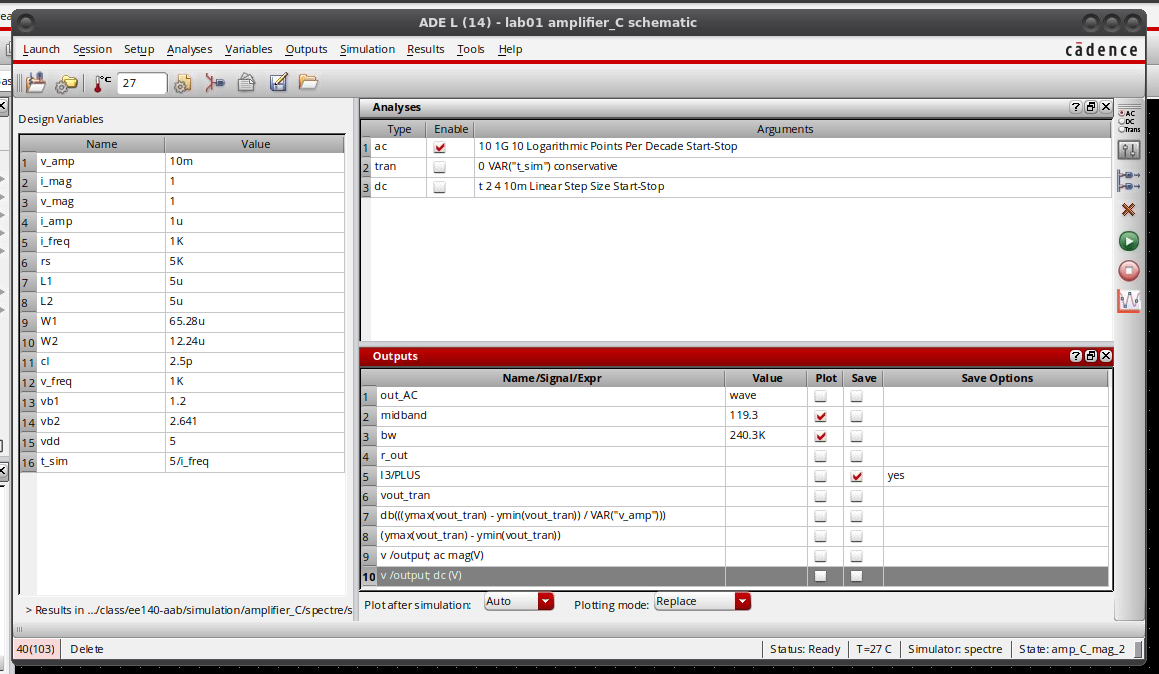
\includegraphics[scale=0.325, center]{c_gain_bw_new2.png}
\newpage\noindent
Since we are very close with the gain I decided it was time to check the output swing.  Below is a screenshot:\\[0.1cm]
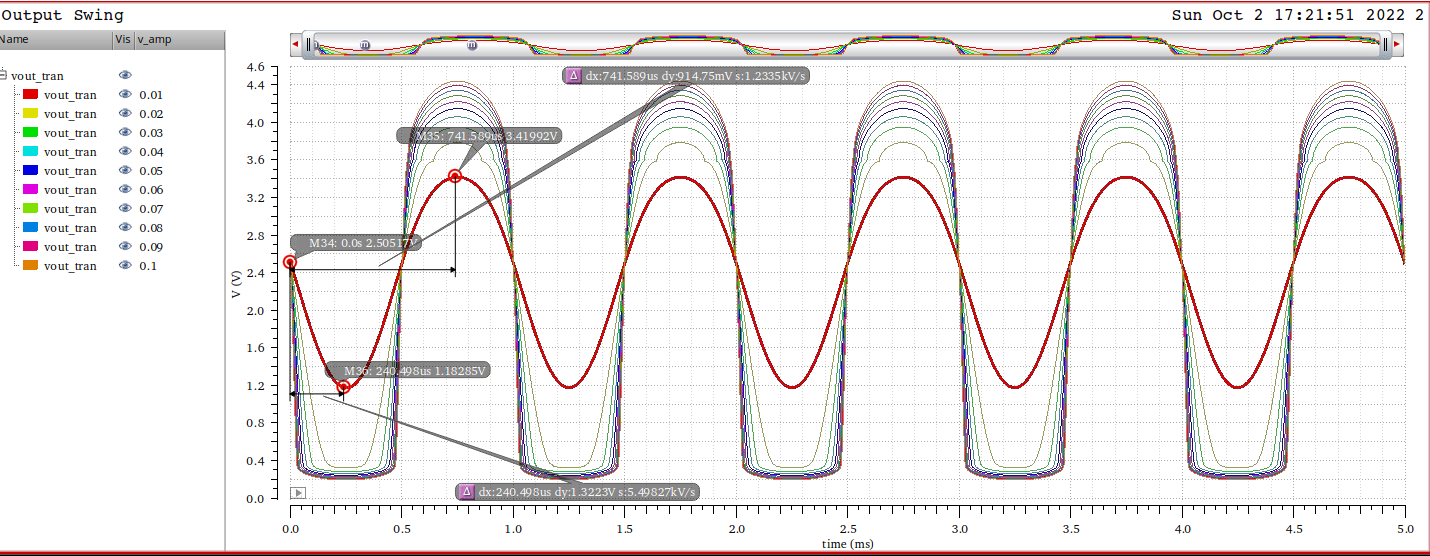
\includegraphics[scale=0.325, center]{c_swing_init.png}\\
Unfortunately we only have an output swing of ~$2\,V$, so other adjustments will need to be made.

At this point I have decided to run trials and organize the results into a table in order to better analyze the data, and find out the best way to turn the dials in order to meet the specs.  Once again I will omit the calculations and pictures, because it is the same procedure as above.  After I have a final result of either meeting or not meeting the requirements, I will discuss my reasoning.  Below is a table of the trials run to meet all the requirements:
\begin{table}[H]
\centering
\setlength{\tabcolsep}{4pt}
\renewcommand{\arraystretch}{1.25}
\begin{tabular}{|c|c|c|c|c|c|c|c|c|c|}
    \hline
    $g_{m_1}$ & $\Delta V_1$ & $\Delta V_2$ & $V_{B1}$ & $V_{B2}$ & $W_1$ & $W_2$ & Gain & BW & Swing\\
    \hline
    $0.47\,mS$ & $0.444\,V$ & $1.556\,V$ & $1.244\,V$ & $2.644\,V$ & $58.9\,\mu m$ & $14.43\,\mu m$ & $109.4\,V/V$ & $262.1\,kHz$ & N/A\\
    \hline
    $0.47\,mS$ & $0.4\,V$ & $1.6\,V$ & $1.2\,V$ & $2.641\,V$ & $65.278\,\mu m$ & $12.24\,\mu m$ & $119.3\,V/V$ & $240.3\,kHz$ & $2\,V$\\
    \hline
    $0.47\,mS$ & $0.3\,V$ & $1.2\,V$ & $1.1\,V$ & $3.021\,V$ & $87.037\,\mu m$ & $16.319\,\mu m$ & $173.6\,V/V$ & $165.8\,kHz$ & $2.6\,V$\\
    \hline
    $0.55\,mS$ & $0.3\,V$ & $1.0\,V$ & $1.1\,V$ & $3.224\,V$ & $101.851\,\mu m$ & $27.50\,\mu m$ & $181.9\,V/V$ & $181.8\,kHz$ & $2.8\,V$\\
    \hline
    $0.65\,mS$ & $0.3\,V$ & $0.9\,V$ & $1.1\,V$ & $3.325\,V$ & $120.37\,\mu m$ & $40.123\,\mu m$ & $185.6\,V/V$ & $204.7\,kHz$ & $2.9\,V$\\
    \hline
    $0.6\,mS$ & $0.3\,V$ & $0.8\,V$ & $1.1\,V$ & $3.425\,V$ & $111.111\,\mu m$ & $46.875\,\mu m$ & $187.5\,V/V$ & $189.3\,kHz$ & $3.0\,V$\\
    \hline
\end{tabular}
\caption{Results of trials to tune the amplifier.}
\end{table}

\noindent
After realizing that I needed to increase the voltage swing, I decided to lower $\Delta V_1$ and $\Delta V_2$, because $\Delta V_1 + \Delta V_2 \leq 2\,V$ was an upper bound for the swing, and increasing the spread between $V_{B1}$ and $V_{B2}$ should help to improve it.  This worked, and also had the added effect of increasing the gain at the cost of reducing the BW.  Although the output swing, while improved, was still not satisfied.  The same strategy of decreasing $\Delta V_1$ and $\Delta V_2$ to improve swing was used, while at the same time increasing $g_m$ to compensate for the reduction in BW.  The initial $g_m$ we found was a lower bound, so increasing it was acceptable.  This method was done in small increments until all requirements were met.  After six trials I was able to successfully tune the amplifier.  
\newpage\noindent
Below is the gain and BW with our with our final values that allow this amplifier to meet all the specs.\\[0.1cm]
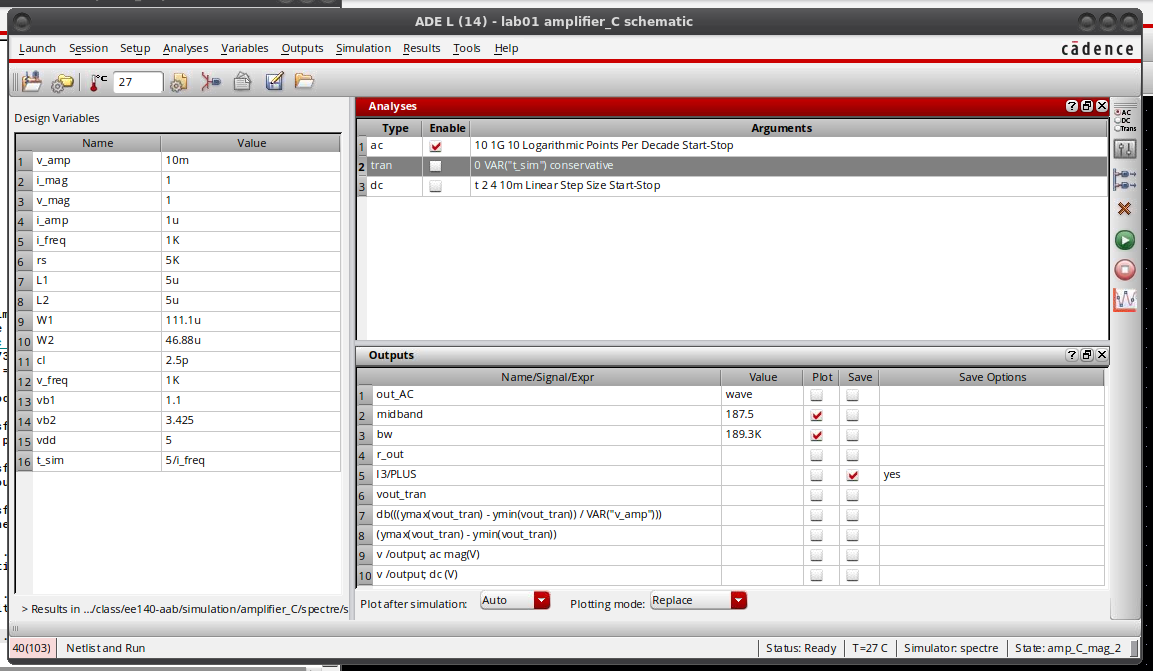
\includegraphics[scale=0.35, center]{c_gain_bw.png}\\[0.25cm]
Below is the output resistance.\\[0.1cm]
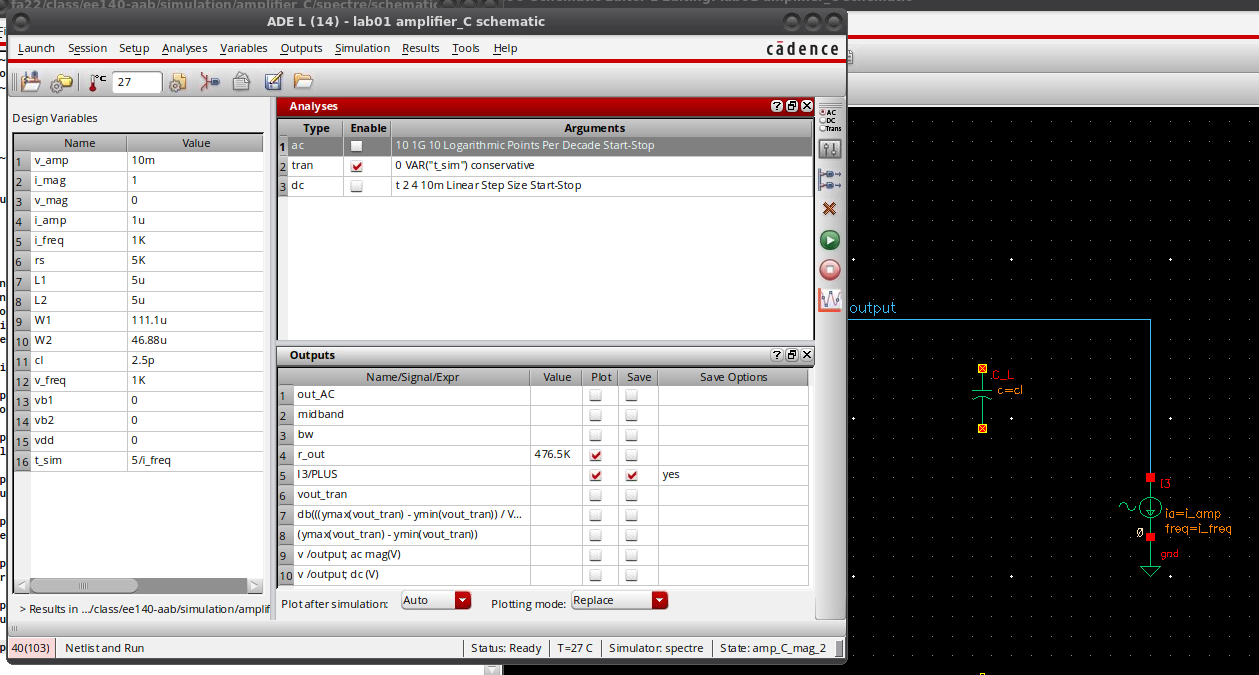
\includegraphics[scale=0.35, center]{c_rout.png}
\newpage
Below is a transient plot of the output swing.\\[0.1cm]
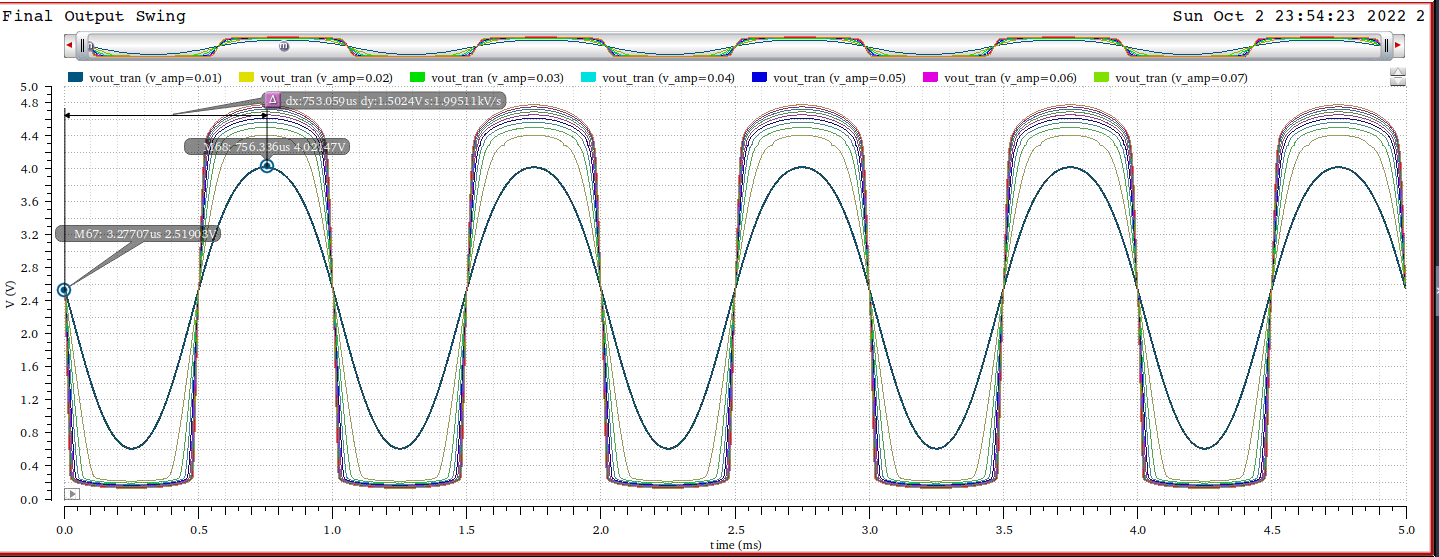
\includegraphics[scale=0.35, center]{c_swing.png}\\[0.25cm]
Below is a Bode plot of the gain and BW.\\[0.1cm]
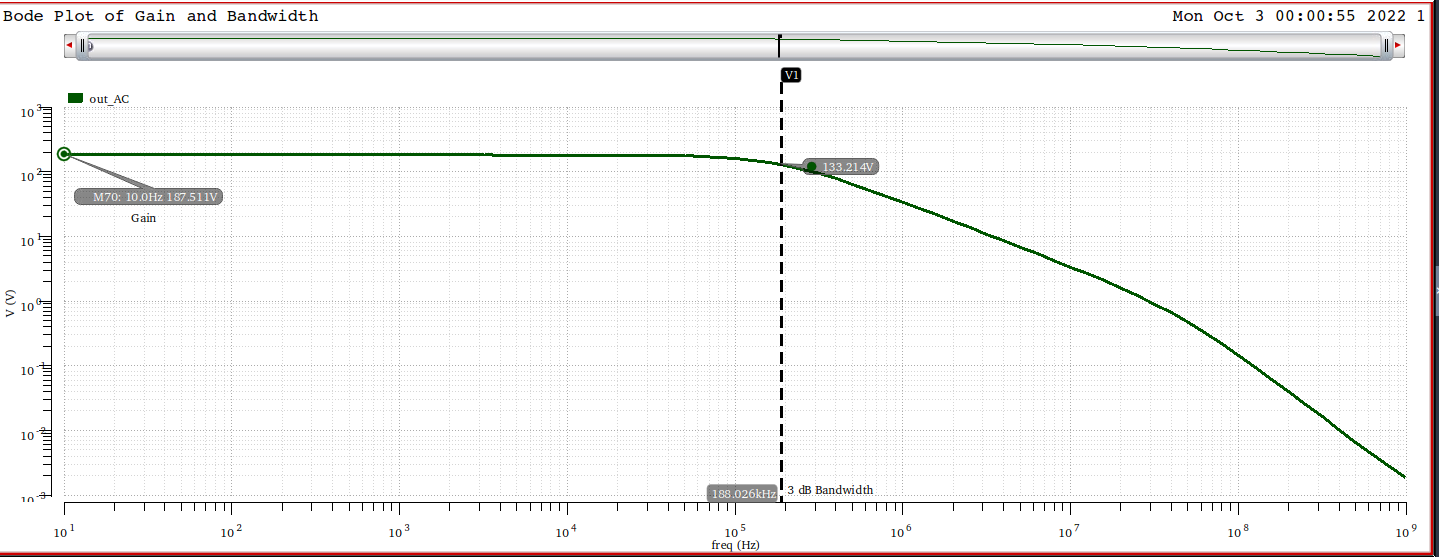
\includegraphics[scale=0.35, center]{c_bode.png}
\newpage
%%%%%%%%%%%%%%%%%%%%%%%%%%%%%%%%%%%%%%%%
%                 RESULTS              %
%%%%%%%%%%%%%%%%%%%%%%%%%%%%%%%%%%%%%%%%
\subsubsection{Results}
Below is a table of results for both the hand calculations and simulated values:

\begin{table}[H]
\centering
\setlength{\tabcolsep}{20pt}
\renewcommand{\arraystretch}{1.5}
\begin{tabular}{|l|c|c|}
    \hline
    \textbf{\textit{Parameter}} & \textbf{\textit{Hand Calculated Value}} & \textbf{\textit{Simulated Value}}\\
    \hline
    $\left|\text{\textit{Voltage Gain}}\right|$ & $150.015\,V/V$ & $187.5\,V/V$\\
    \hline
    \textit{Bandwidth} & $199.98\,kHz$ & $189.3\,kHz$\\
    \hline
    \textit{Output Resistance} & $318.34\,k\Omega$ & $476.5\,k\Omega$\\
    \hline
    \textit{Voltage Swing} & $3\,V$ & $3\,V$\\
    \hline
\end{tabular}
\caption{Results for MOS amplifier in \textit{Part II}.}
\end{table}
\noindent
\underline{\textbf{\textit{Summary of Results}}}\\[0.25cm]
In this case the discrepancies of hand calculated values compared to the simulated results arise from the fact that we were trying to find bounds on values, and adding in headroom in order to find a proper biasing point.  Ignoring body effect and CLM also probably heightened this error.  Since $V_{B2}$ was required to be so precisely tuned in order for both transistors to operate in saturation, it is impractical to expect being able to have precise hand calculations with this setup.  Thus, we were required to sweep the voltage of $V_{B2}$ for precise mid-rail biasing in order to get a proper gain.

We also notice that the output resistance of this amplifier is much larger than the CS amplifier used in Part I.  At first this seems strange, because we have a voltage amplifier.  In a good voltage amplifier that is driving a load, we typically desire a high load impedance, but a low output impedance.  However, this makes sense because the expression for the gain that we derived is highly dependent on the output resistance.  The large gain severely reduced the BW from the CS amplifier, but that is to be expected.  The balance of speed and gain is usually the trade-off you make in designing amplifiers.
\newpage
%%%%%%%%%%%%%%%%%%%%%%%%%%%%%%%%%%%%%%%%%%%%%%%%%%%%%%
%                       TASK B                       %
%%%%%%%%%%%%%%%%%%%%%%%%%%%%%%%%%%%%%%%%%%%%%%%%%%%%%%
\subsection{Adding a Current Mirror}
\textbf{\emph{Find: }} Replace $V_{B2}$ with a current mirror to produce a more stable amplifier.\\[0.25cm]
\noindent
\textbf{\emph{Solution: }}
%%%%%%%%%%%%%%%%%%%%%%%%%%%%%%%%%%%%%%%%
%            HAND CALCULATIONS         %
%%%%%%%%%%%%%%%%%%%%%%%%%%%%%%%%%%%%%%%%
\subsubsection{Hand Calculations}
For the hand calculations we will again be ignoring the body effect and channel length modulation.  We will also assume that $C_L$ is the dominant pole, which will be checked in the hand calculations to make sure our assumption was correct.\\[0.25cm]
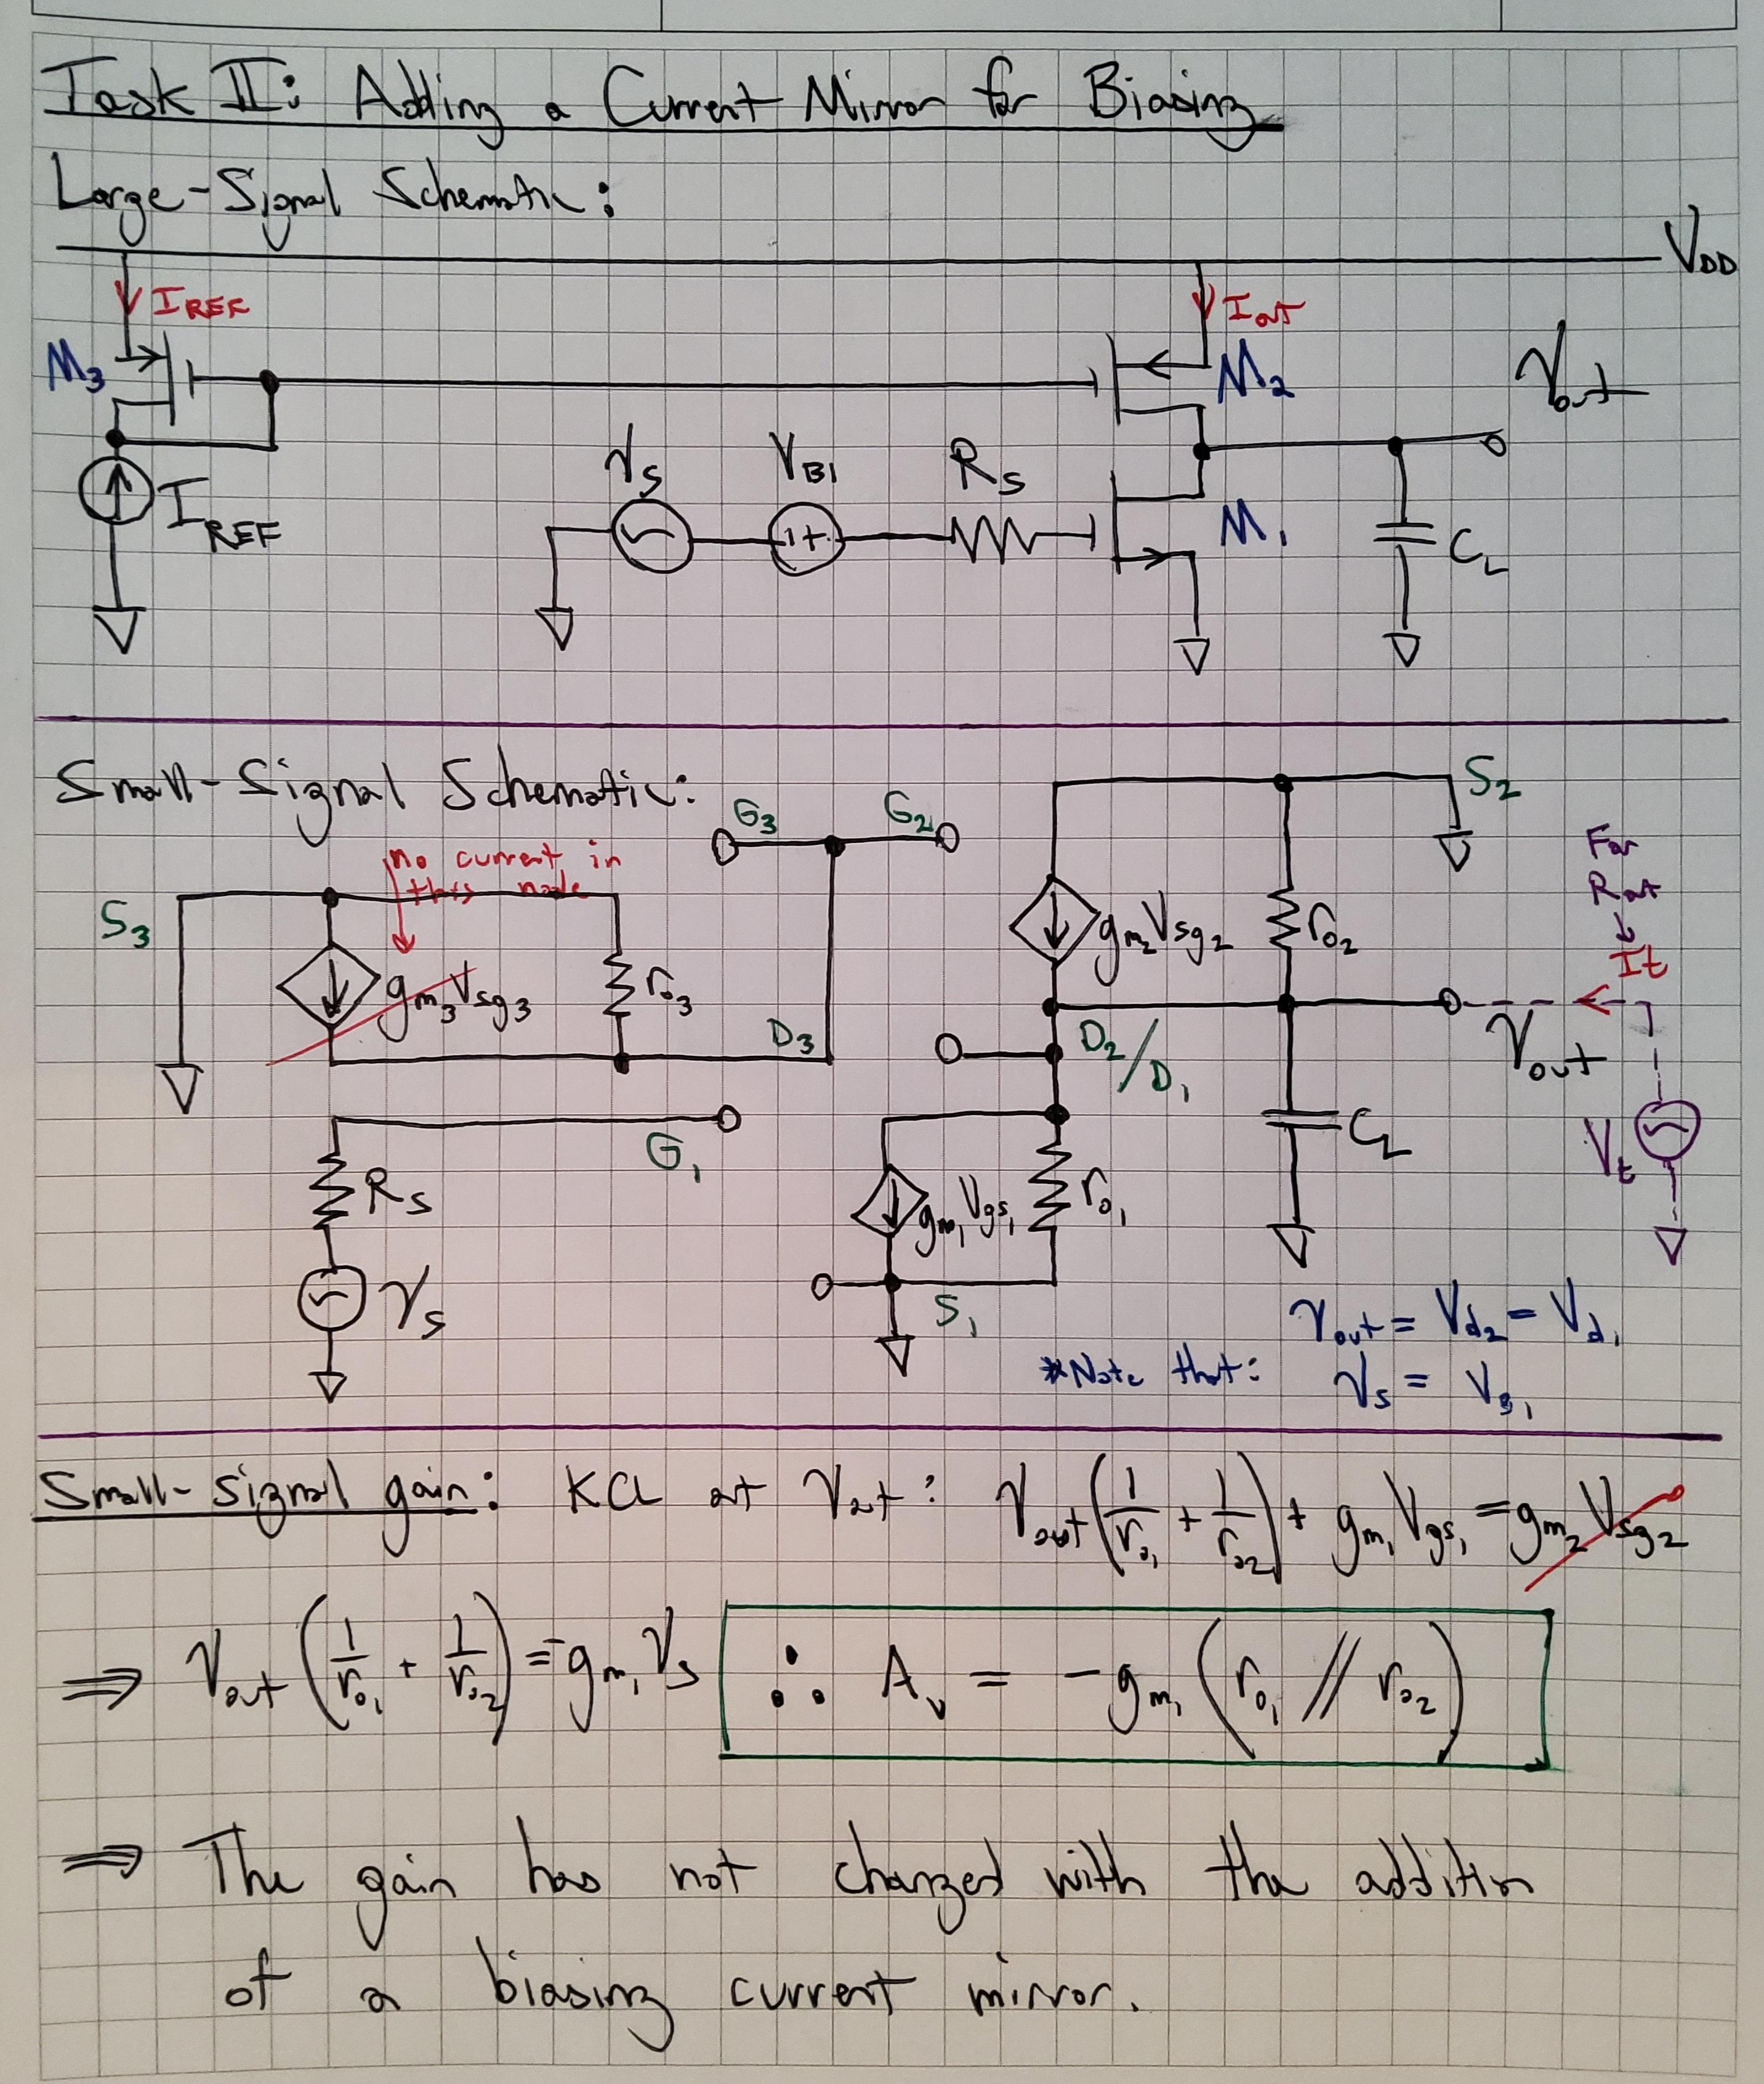
\includegraphics[scale=0.14, center]{p2b_1.jpg}\\
\newpage
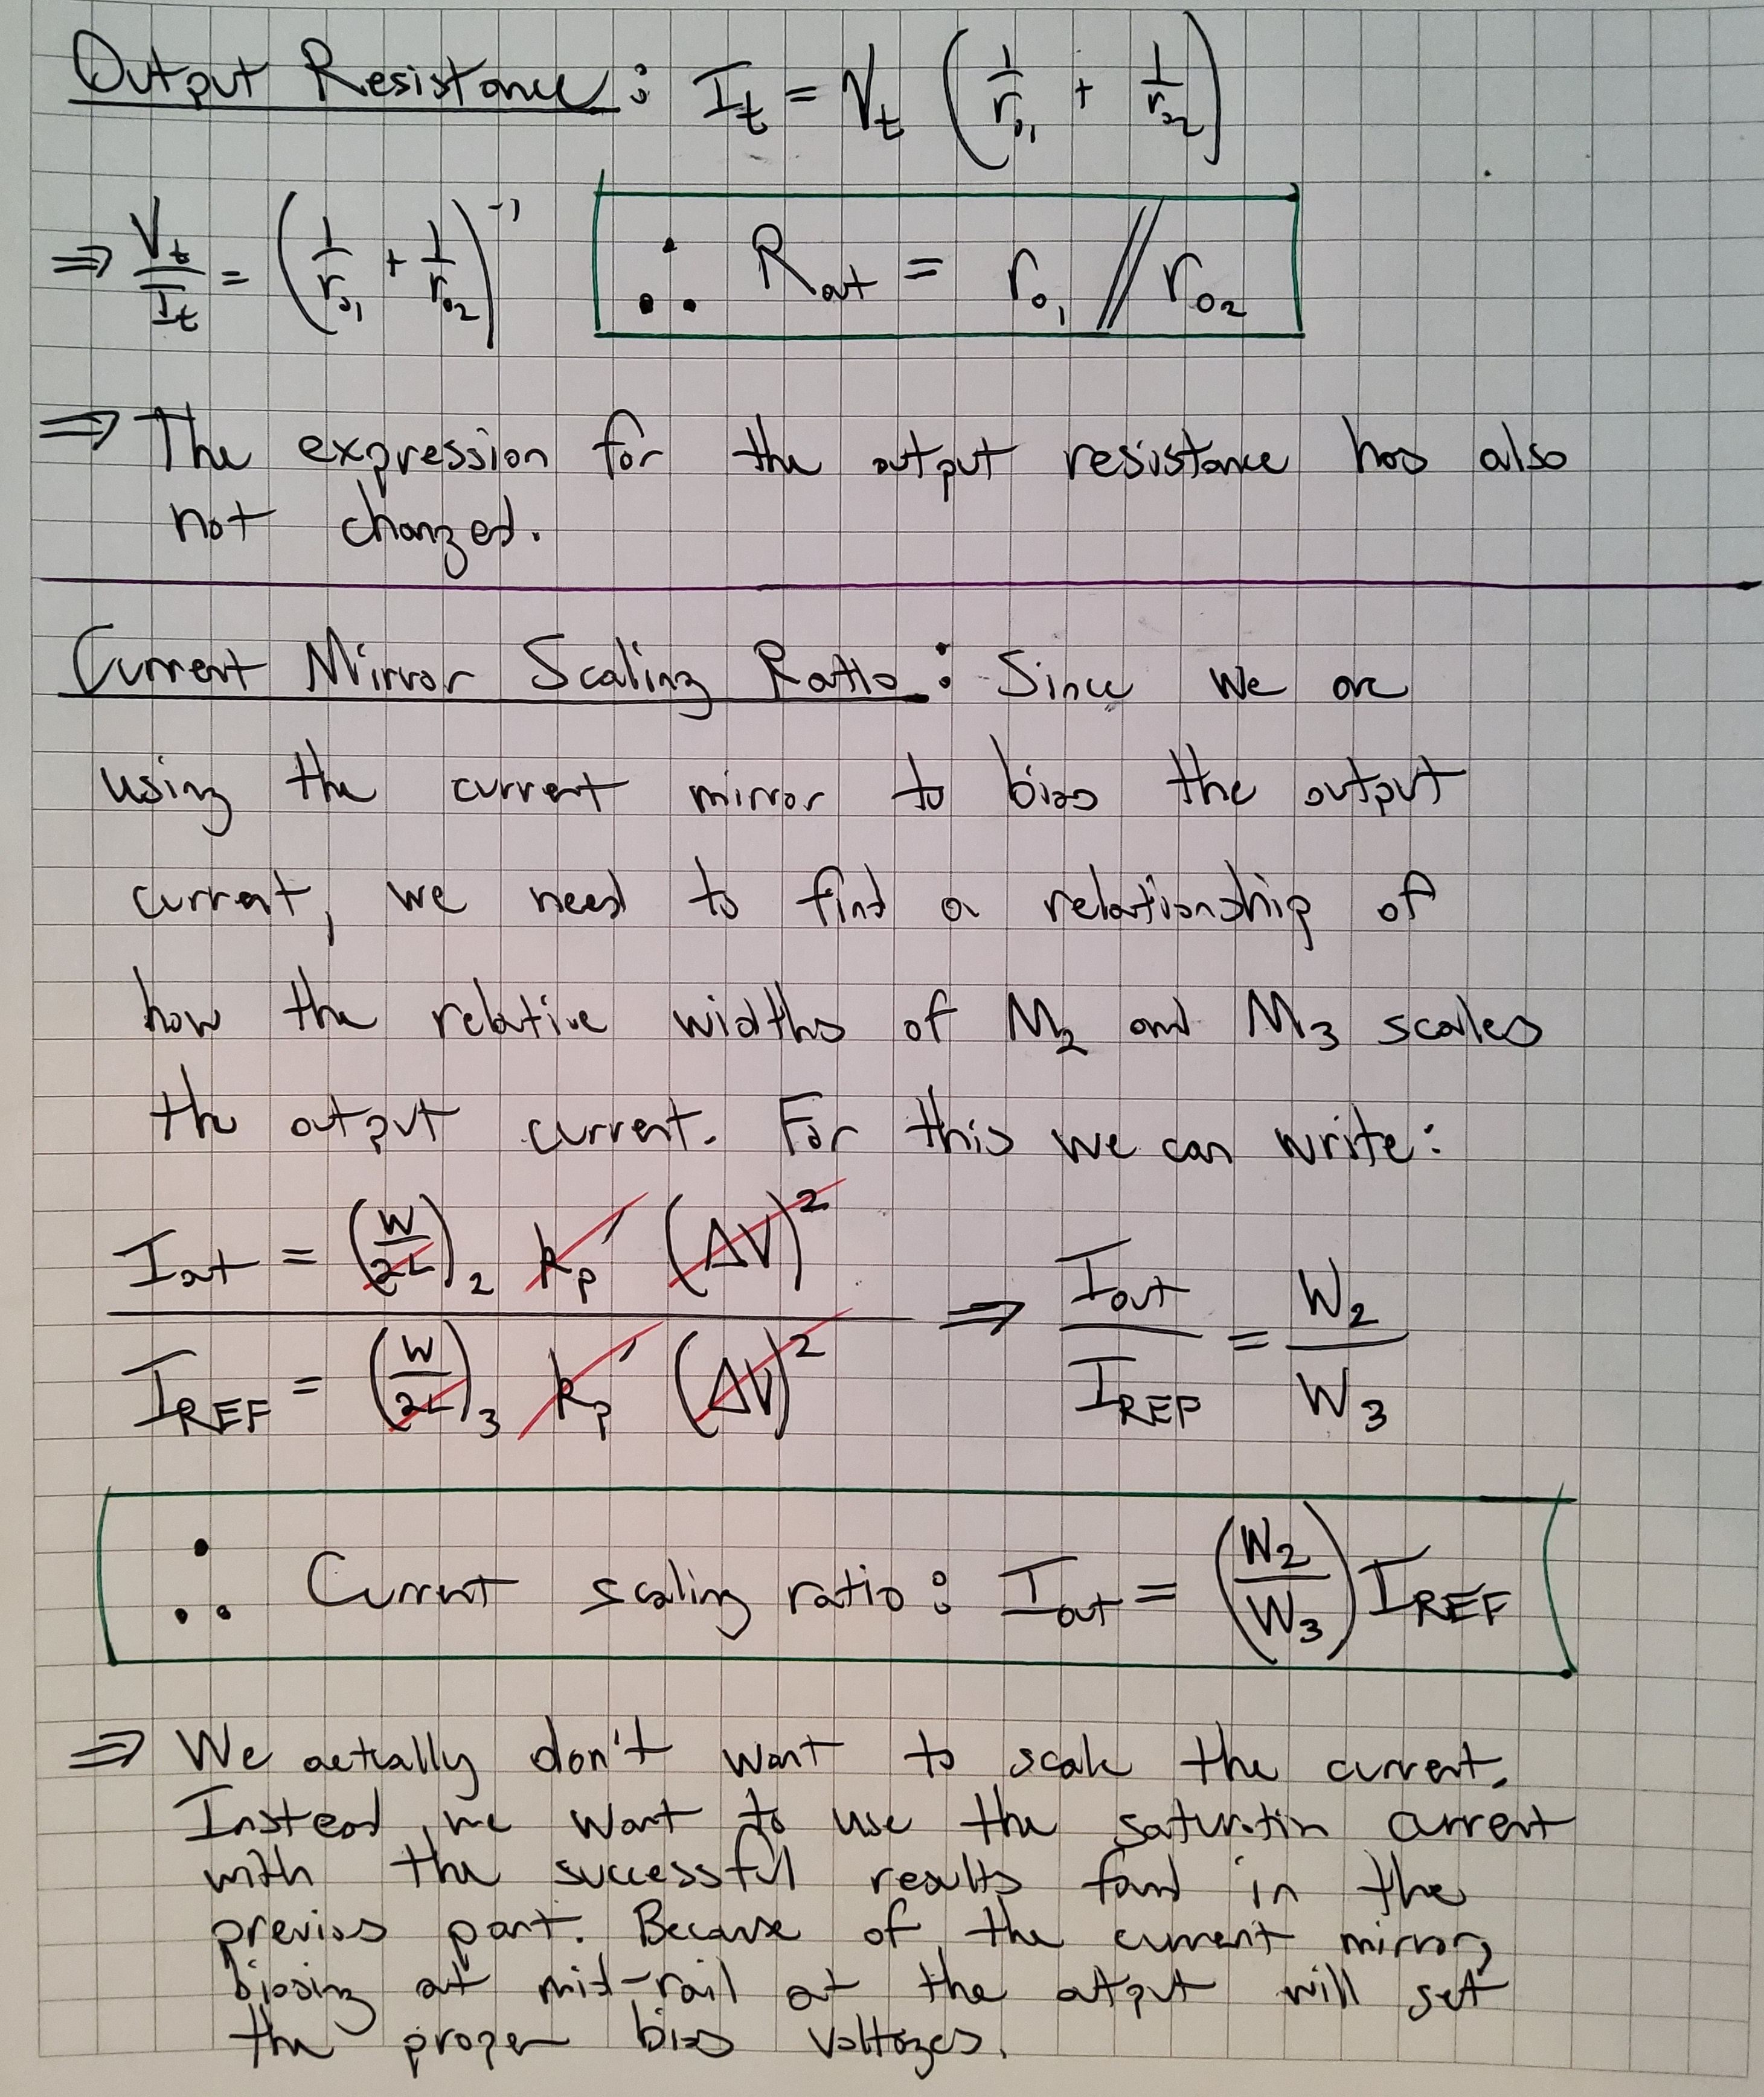
\includegraphics[scale=0.165, center]{p2b_2.jpg}\\
\newpage
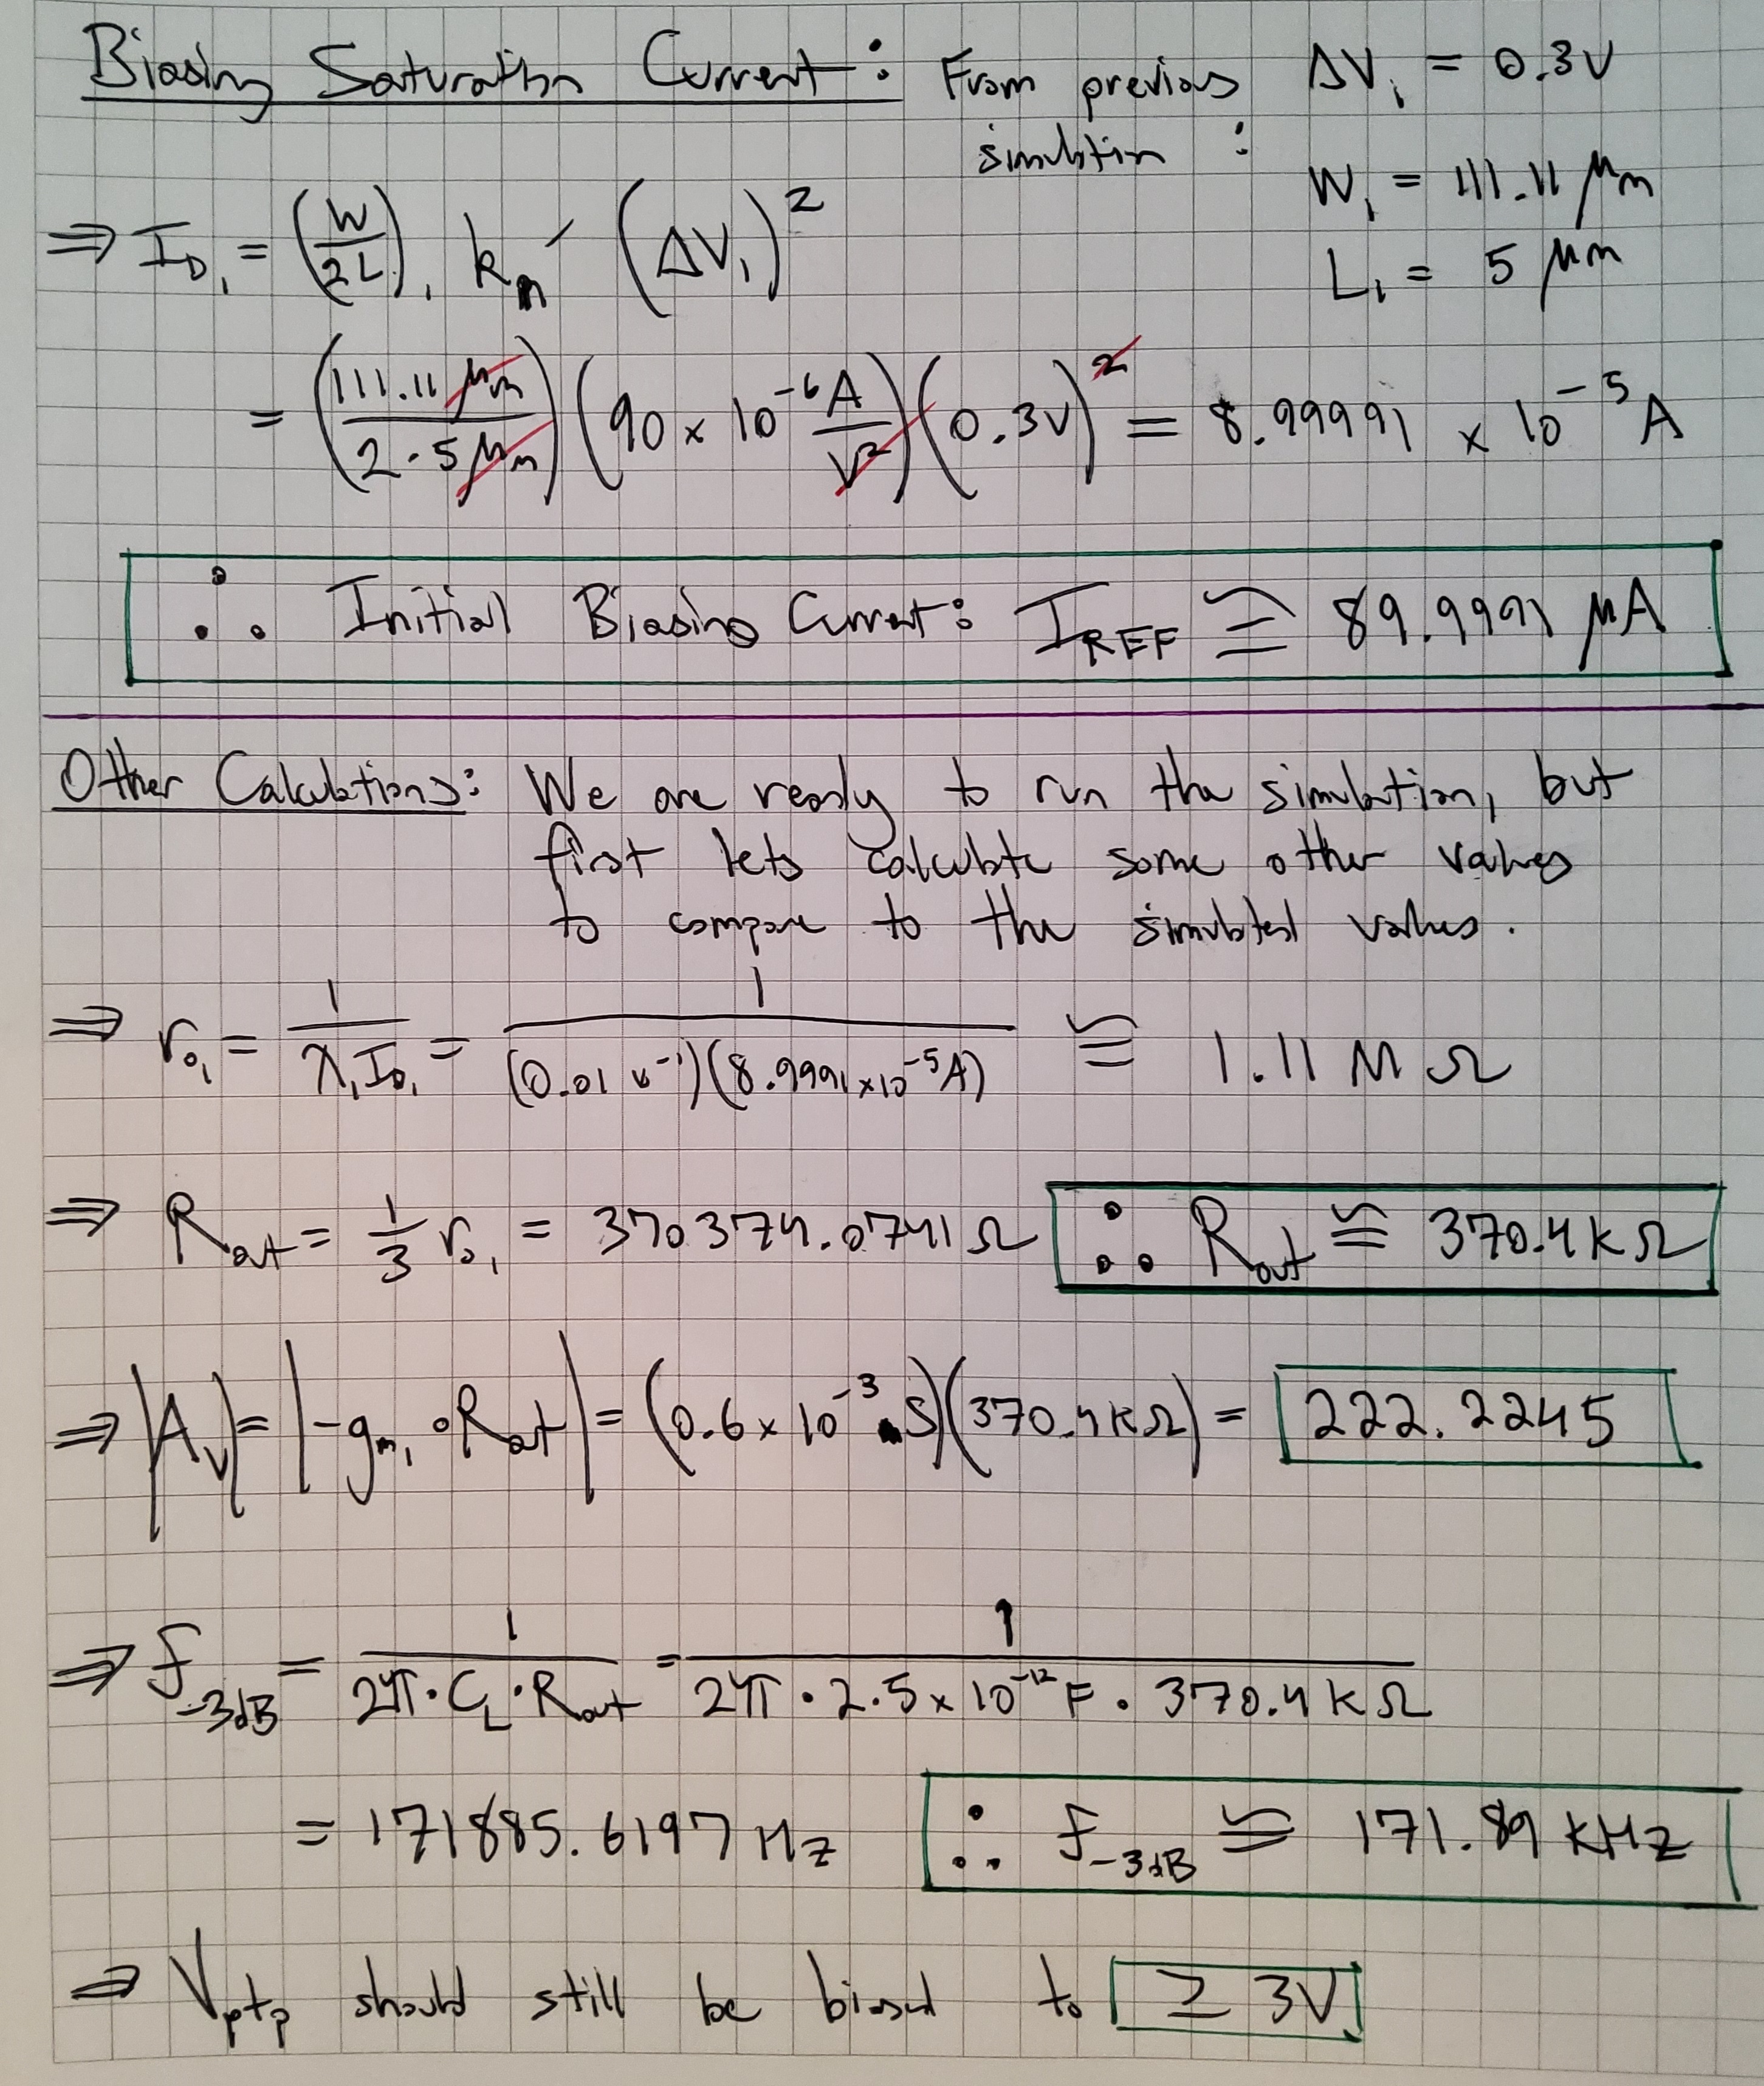
\includegraphics[scale=0.165, center]{p2b_3.jpg}\\
\newpage
%%%%%%%%%%%%%%%%%%%%%%%%%%%%%%%%%%%%%%%%
%               SIMULATION             %
%%%%%%%%%%%%%%%%%%%%%%%%%%%%%%%%%%%%%%%%
\subsubsection{Simulation}
Below is the internal schematic of the amplifier with the added current mirror used for simulation:\\[0.1cm]
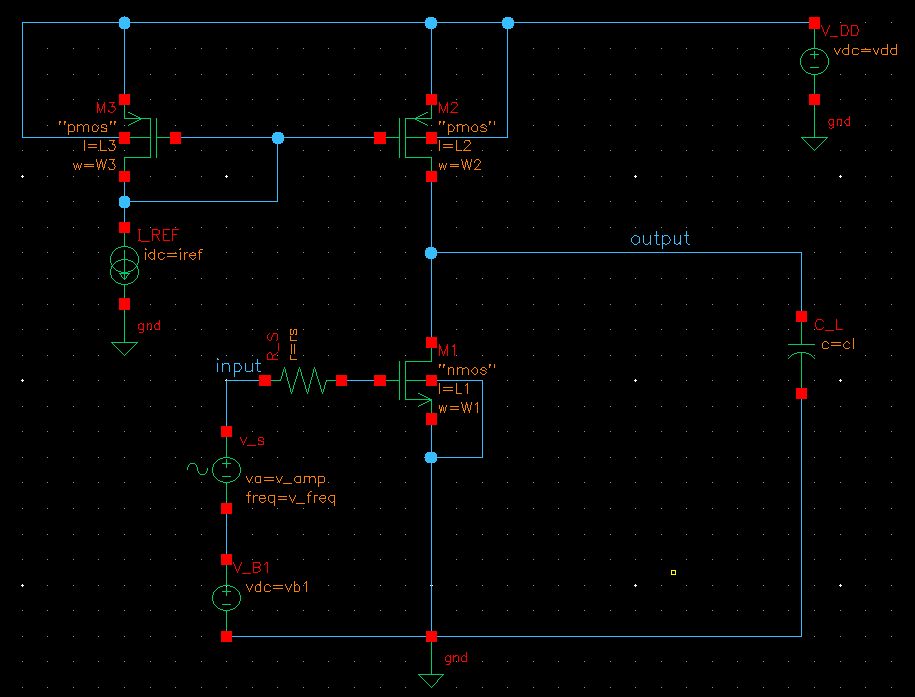
\includegraphics[scale=0.4, center]{d_internal.png}\\[0.25cm]
Below is the gain and bandwidth using our hand calculated numbers:\\[0.1cm]
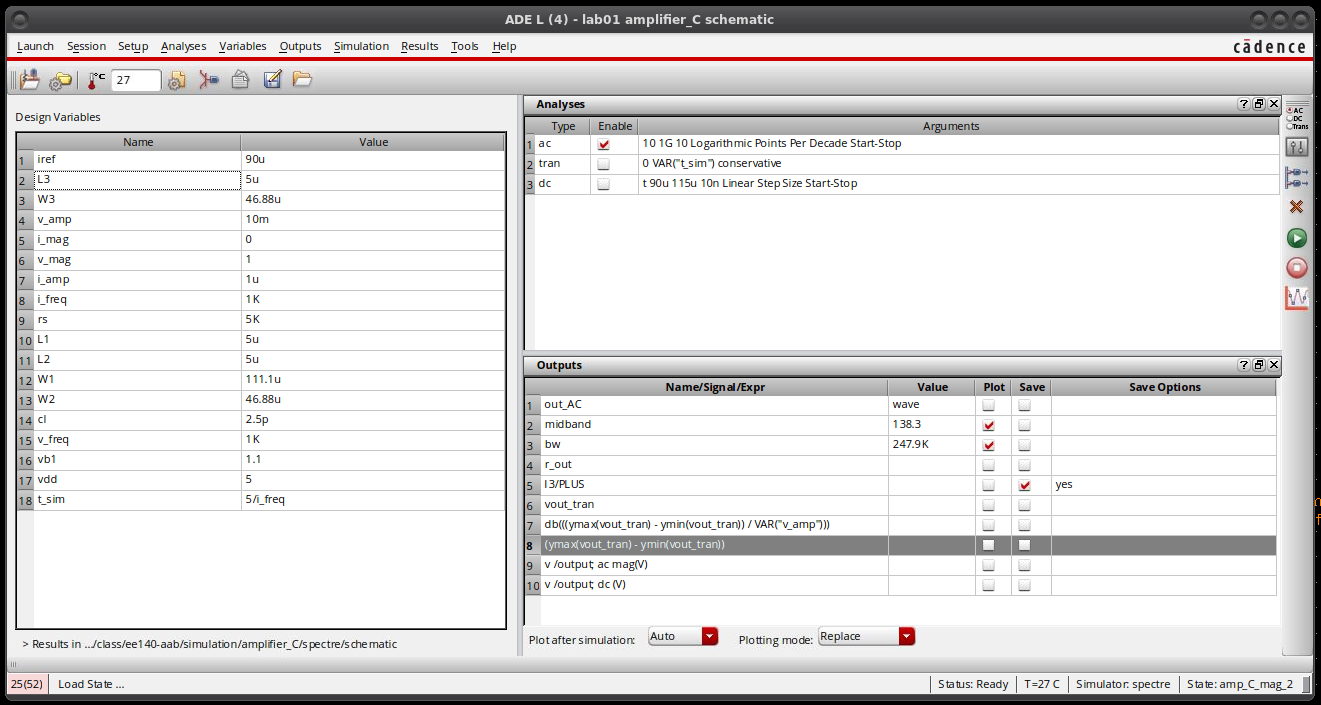
\includegraphics[scale=0.3, center]{d_gain_bw_init.png}
\newpage\noindent
We are actually already meeting the gain and BW specs, but the amplifier is almost certainly not operating at its peak performance levels.  I decided to observe the DC voltages, because I still want the output voltage to be at mid-rail for optimum performance, which is $V_{DD} / 2 = 2.5\,V$.  Below is a screenshot of the current node voltages:\\[0.1cm]
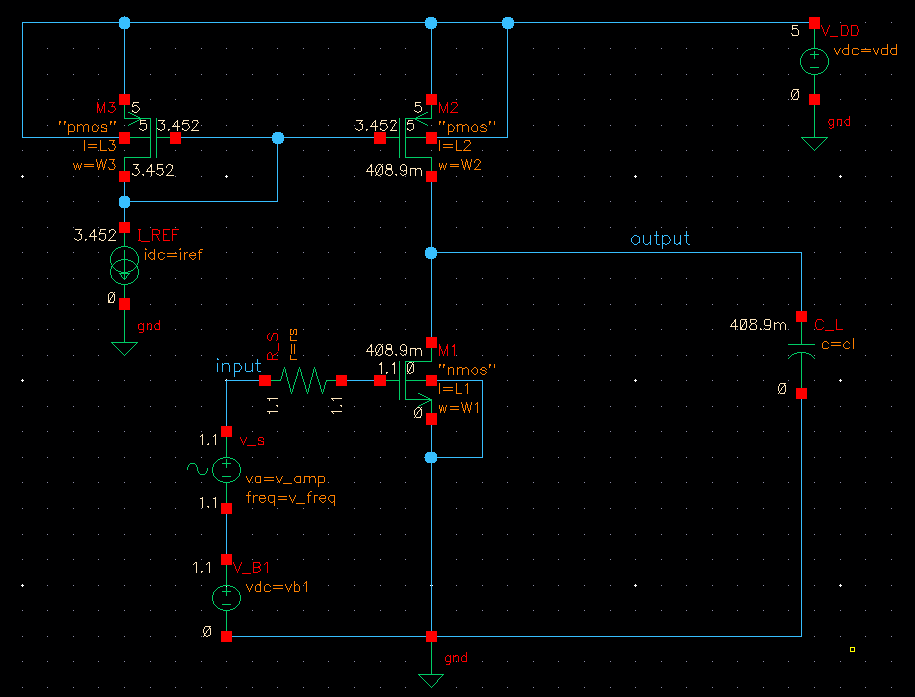
\includegraphics[scale=0.4, center]{d_dc_voltage.png}\\[0.25cm]
As we can see, the output node is well below mid-rail.  Running a sweep of $I_{REF}$ gives us the value to use for a mid-rail bias of $2.5\,V$.  This is shown below.\\[0.1cm]
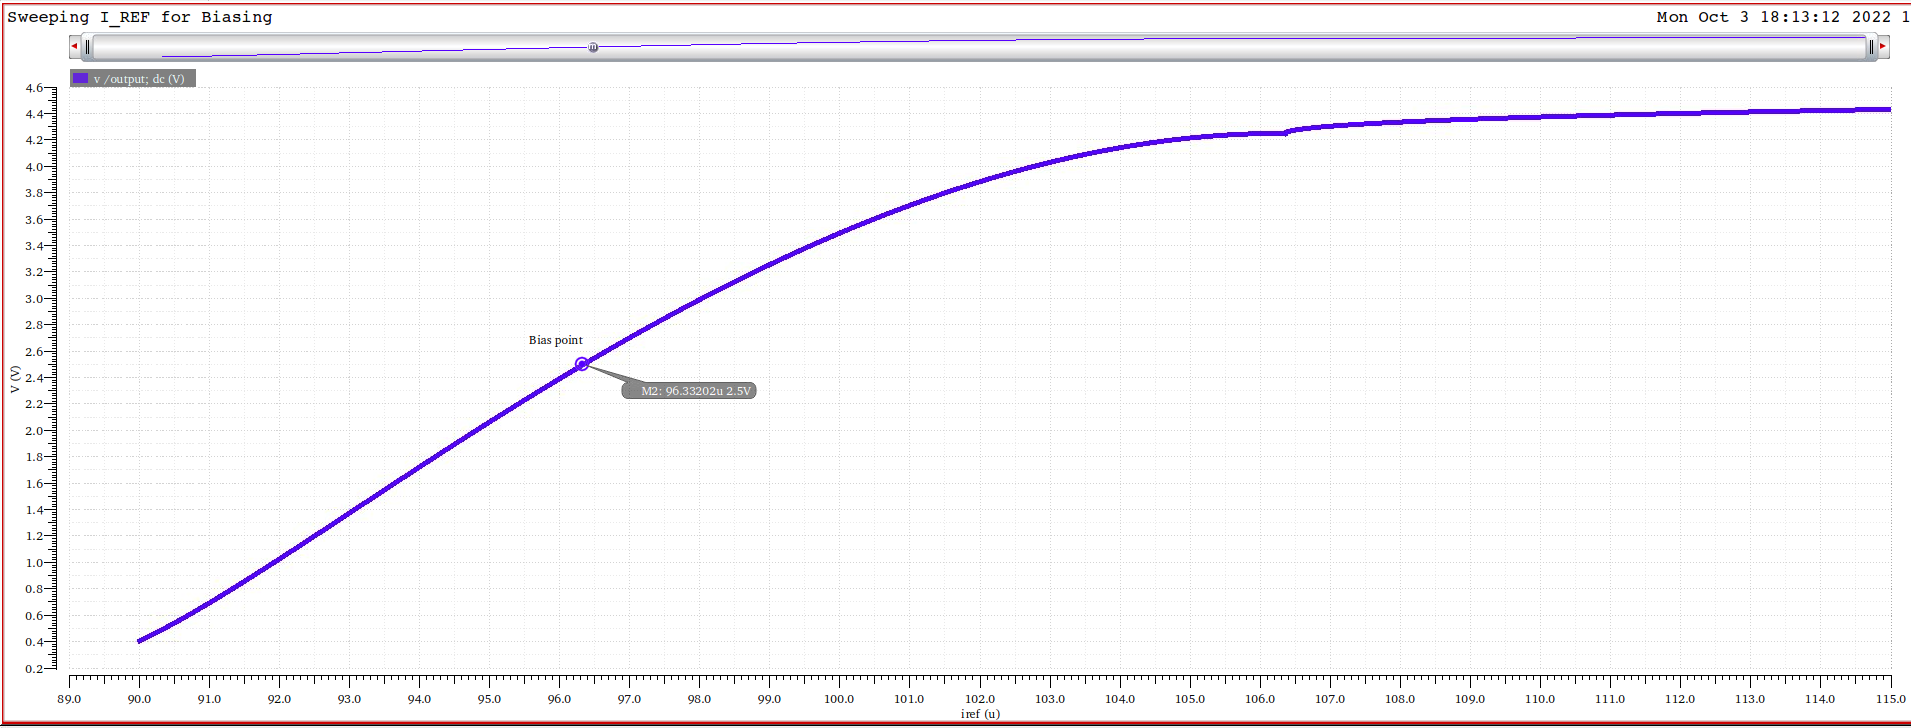
\includegraphics[scale=0.25, center]{d_dc_sweep.png}
\newpage\noindent
Now we run the simulation again with a new $I_{REF}$ bias current of $96.33\,\mu A$.  Below is a screenshot of the new results:\\[0.1cm]
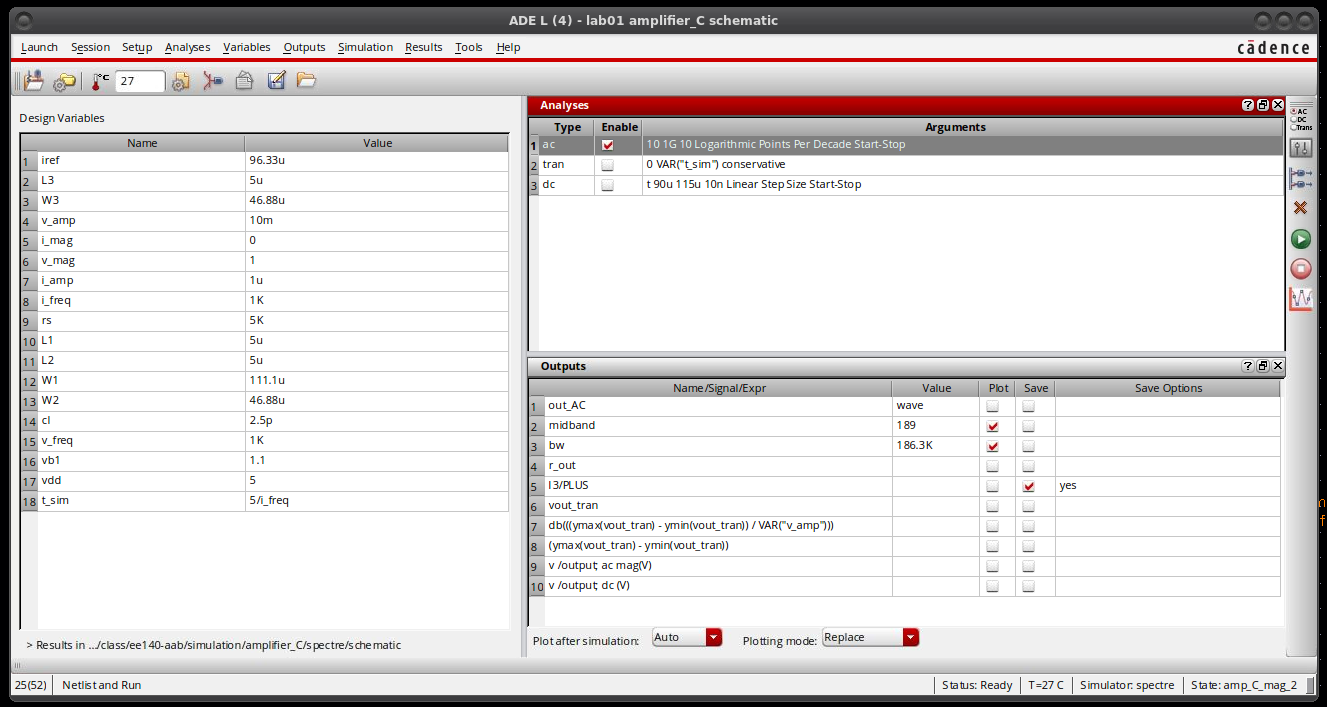
\includegraphics[scale=0.35, center]{d_gain_bw_new.png}\\[0.25cm]
The gain and BW are looking great, now we must check the output swing to ensure that no more adjustments need to be made.  Below is a screenshot of the output swing.\\[0.1cm]
\includegraphics[scale=0.25, center]{d_swing.png}
\newpage\noindent
The output swing requirement is met, and so we are done tuning this amplifier configuration.  Now we will calculate the output resistance.  Below is a screenshot.\\[0.1cm]
\includegraphics[scale=0.35, center]{d_output_res.png}\\[0.25cm]
Below is the Bode plot showing the gain and BW of our fully tuned amplifier that was biased with a current mirror.\\[0.1cm]
\includegraphics[scale=0.25, center]{d_bode.png}
\newpage
%%%%%%%%%%%%%%%%%%%%%%%%%%%%%%%%%%%%%%%%
%                 RESULTS              %
%%%%%%%%%%%%%%%%%%%%%%%%%%%%%%%%%%%%%%%%
\subsubsection{Results}
Below is a table of results for both the hand calculations and simulated values:

\begin{table}[H]
\centering
\setlength{\tabcolsep}{20pt}
\renewcommand{\arraystretch}{1.5}
\begin{tabular}{|l|c|c|}
    \hline
    \textbf{\textit{Parameter}} & \textbf{\textit{Hand Calculated Value}} & \textbf{\textit{Simulated Value}}\\
    \hline
    $\left|\text{\textit{Voltage Gain}}\right|$ & $222.23\,V/V$ & $187.5\,V/V$\\
    \hline
    \textit{Bandwidth} & $171.89\,kHz$ & $189.3\,kHz$\\
    \hline
    \textit{Output Resistance} & $370.4\,k\Omega$ & $476.5\,k\Omega$\\
    \hline
    \textit{Voltage Swing} & $3\,V$ & $3\,V$\\
    \hline
\end{tabular}
\caption{Results for adding a current mirror in \textit{Part II}.}
\end{table}
\noindent
\underline{\textbf{\textit{Summary of Results}}}\\[0.25cm]
Now our hand calculations, while still not matching the simulated results, are a bit more reasonable than previously before we added the current mirror.  The reason for this is because we used the saturation drain current from our previously successful simulated amplifier for the hand calculations.  However, we still needed to run a sweep of the biasing current source which explains the discrepancies.

We can also see that the values of the gain and BW exactly match the original circuit.  This makes sense because we have not changed any other parameters (widths of transistors, and the bias voltage of $V_{B1}$), and we still biased the amplifier to mid-rail.  We simply changed to a more stable method of biasing.
\newpage
%%%%%%%%%%%%%%%%%%%%%%%%%%%%%%%%%%%%%%%%
%             CONCLUSION               %
%%%%%%%%%%%%%%%%%%%%%%%%%%%%%%%%%%%%%%%%
\section{Conclusion}
    \begin{enumerate}[label=(\roman*)]
        \item
        {
        \underline{\textbf{\textit{Part I: Amplifiers in Task A and Task B}}}\\[0.25cm]
        The amplifiers in the first part of this lab gave us a high bandwidth, but a low gain.  The gain was further reduced after adding source degeneration, although this achieves a faster and more stable amplifier with a larger output swing.
        
        After performing the tedious hand calculations, it has become clear to me that approximations should always be made when appropriate to save time and possible errors on complicated algebra.  The hand calculations are a good way to get an idea of the circuit you are dealing with, and at the same time the analysis should result in a fairly accurate estimate of how you expect the amplifier to behave in a simulation.  This most likely becomes more clear as we move on to more complicated topologies.
        }
        \item
        {
        \underline{\textbf{\textit{Part II: MOS Amplifier Design}}}\\[0.25cm]
        It is clear that trying to bias an amplifier of this topology with two voltage sources is not a good way to do it, but it probably is a good way to get fired.  A good way to think about why the bias voltages are so sensitive to small variations is because the saturation currents of the $PMOS$ and $NMOS$ are equal to each other, which means there is only one crossing point where there currents meet, and this is the bias point.  This crossing/bias point is very sensitive to either a slight change in either of the biasing sources, or process parameters such as the transistors not having exactly the same threshold voltage.  Either of these can throw the transistors out of saturation, and we lose most of the gain.
        
        Although we are able to properly tune the amplifier in this simulation, in the real world this is not achievable, and this is the reason for biasing with a different method, such as a current mirror.
        }
        \item
        {
        \underline{\textbf{\textit{Part II: Adding a Current Mirror}}}\\[0.25cm]
        The addition of the current mirror provides stability, and ease of biasing with a simple scaling ratio.  The stability comes from the fact that both transistors remaining in saturation is no longer dependent on a precise bias point from two voltage sources.
        
        In the real world, I would probably take the biasing a step further by reducing the width of transistor $M_3$ in order to reduce power consumption.  However, for the purposes of this lab our final result was acceptable and met all of the required specifications quite comfortably.  
        }
    \end{enumerate}
\newpage
%%%%%%%%%%%%%%%%%%%%%%%%%%%%%%%%%%%%%%%%%%%%%%%%%%%%%%%%%%%%%%%%%%%%%%%%%%%%%%%%%%%%%%%%%%%%%%%%%%%%%%%%%%%
%                                             APPENDIX                                                    %
%%%%%%%%%%%%%%%%%%%%%%%%%%%%%%%%%%%%%%%%%%%%%%%%%%%%%%%%%%%%%%%%%%%%%%%%%%%%%%%%%%%%%%%%%%%%%%%%%%%%%%%%%%%
\appendix
%%%%%%%%%%%%%%%%%%%%%%%%%%%%%%%%%%%%%%%%%%%%%%%%%%%%%%%%%%%%%%%%%%%%%%%%%%%%%%%%%%%%%%%%%%%%%%%%%%%%%%%%%%%
%                                APPENDIX A: GLOSSARY OF EQUATIONS                                        %
%%%%%%%%%%%%%%%%%%%%%%%%%%%%%%%%%%%%%%%%%%%%%%%%%%%%%%%%%%%%%%%%%%%%%%%%%%%%%%%%%%%%%%%%%%%%%%%%%%%%%%%%%%%
\newpage
\section{Appendix: Glossary of Equations}
    \begin{flalign}
        &&\Aboxed{\phi_{bi} &= \frac{kT}{q} \cdot ln\;\bigg( \frac{N_D \cdot N_A}{{n_i}^2} \bigg)}
        &&\textit{Built-in potential, $PN$-junction}
        \label{eq:phi_bi}
    \end{flalign}

    \begin{flalign}
        &&\Aboxed{W_{dep} &= \sqrt{\frac{2\epsilon_s \left(\phi_{bi} - V_{applied}\right)}{q}
                        \cdot \Bigg( \frac{1}{N_A} + \frac{1}{N_D} \Bigg)}}
        &&\textit{Depletion region width, total}
        \label{eq:total_dep}
    \end{flalign}        

    \begin{flalign}
        &&\Aboxed{C_{dep} &= A \left(\frac{\epsilon_s}{W_{dep}}\right)}
        &&\textit{Junction capacitance}
        \label{eq:junc_cap}
    \end{flalign}

    \begin{flalign}
        &&\Aboxed{I_{DS,sat} &= \left(\frac{W}{2L}\right) \mu_n\,C_{ox}
                         {\big(V_{GS} - V_{T_n}\big)}^2 (1 + \lambda V_{DS})}
        &&\textit{$NMOS$ saturation current}
        \label{eq:mosfet_ids_nmos_sat}\\[0.25cm]
        &&\Aboxed{I_{DS,tri} &= \left(\frac{W}{L}\right) \mu_n\,C_{ox}
                            \left(V_{GS} - V_{T_n} - \frac{V_{DS}}{2}\right) V_{DS}}
        &&\textit{$NMOS$ triode current}
        \label{eq:mosfet_ids_nmos_tri}\\[0.25cm]
        &&\Aboxed{I_{SD,sat} &= \left(\frac{W}{2L}\right) \mu_p\,C_{ox}
                         {\big(V_{SG} - \left|V_{T_p}\right|\big)}^2 (1 + \lambda V_{SD})}
        &&\textit{$PMOS$ saturation current}
        \label{eq:mosfet_ids_pmos_sat}\\[0.25cm]
        &&\Aboxed{I_{SD,tri} &= \left(\frac{W}{L}\right) \mu_p\,C_{ox}
                            \left(V_{SG} - \left|V_{T_p}\right| - \frac{V_{SD}}{2}\right) V_{SD}}
        &&\textit{$PMOS$ triode current}
        \label{eq:mosfet_ids_pmos_tri}
    \end{flalign}

    \begin{flalign}
        &&\Aboxed{r_o &= \frac{1}{\frac{W\,\mu\,C_{ox}}{2L}{(V_{GS} - V_T)}^2\,\lambda}
        \approx \frac{1}{\lambda\,I_{DS}}}
        &&\textit{Output resistance for MOSFET}
        \label{eq:mos_outresistance}
    \end{flalign}

    \begin{flalign}
        &&\Aboxed{g_m &= \left(\frac{W}{L}\right)\mu\,C_{ox}(V_{{DS}_{sat}})
        = \sqrt{\left(\frac{2W}{L}\right)\mu\,C_{ox} I_{DS}}
        = \frac{2 \cdot I_{DS}}{V_{GS} - V_T}}
        &&\textit{Transconductance for MOSFET}
        \label{eq:mos_transconductance}
    \end{flalign}

    \begin{flalign}
        &&\Aboxed{V_{GS} = V_T + \sqrt{\frac{2\,I_{DS}}{\frac{W}{L} \mu C_{ox}}} = V_T + V_{OD}}
        &&\textit{Gate-source condition, diode-connected MOSFET}
        \label{eq:mos_gate_cond}
    \end{flalign}
%%%%%%%%%%%%%%%%%%%%%%%%%%%%%%%%%%%%%%%%%%%%%%%%%%%%%%%%%%%%%%%%%%%%%%%%%%%%%%%%%%%%%%%%%%%%%%%%%%%%%%%%%%%
%                                APPENDIX B: GLOSSARY OF TABLES                                           %
%%%%%%%%%%%%%%%%%%%%%%%%%%%%%%%%%%%%%%%%%%%%%%%%%%%%%%%%%%%%%%%%%%%%%%%%%%%%%%%%%%%%%%%%%%%%%%%%%%%%%%%%%%%
\newpage
\section{Appendix: Glossary of Tables}
    \begin{table}[H]
    \centering
    \setlength{\tabcolsep}{20pt}
    \renewcommand{\arraystretch}{1.5}
    \begin{tabular}{|l|c|c|c|}
        \hline
        \textbf{Transistor Type}  &  \textbf{Cut-off} & \textbf{Triode} & \textbf{Saturation}\\
        \hline
        \textit{NMOS} & $V_{GS} \leq V_{T_n}$
                        & $V_{DS} \leq V_{GS} - V_{T_n}$
                        & $V_{DS} > V_{GS} - V_{T_n}$\\
        \hline
        \textit{PMOS} & $V_{SG} \leq \left|V_{T_p}\right|$
                        & $V_{SD} \leq V_{SG} - \left|V_{T_p}\right|$
                        & $V_{SD} > V_{SG} - \left|V_{T_p}\right|$\\
        \hline
    \end{tabular}
    \caption{Conditions for MOSFET regions of operation.
    \label{tab:mosfet_op}} 
    \end{table}

    \begin{table}[H]
    \centering
    \setlength{\tabcolsep}{20pt}
    \renewcommand{\arraystretch}{1.5}
    \begin{tabular}{|l|c|c|}
        \hline
        \textbf{Description}  &  \textbf{Symbol} & \textbf{Value}\\
        \hline
        Elementary charge & $q$ & $\num{1.60218e-19}\,C$\\
        \hline
        Electron volt & $eV$ & $\num{1.60218e-19}\,J$\\
        \hline
        Boltzmann's constant & $k$ & $\num{1.38066e-23}\,J/K$\\
        \hline
        Free electron mass & $m_0$ & $\num{9.1095e-31}\,kg$\\
        \hline
        Permittivity in vacuum & $\epsilon_0$ & $\num{8.85418e-12}\,F/m$\\
        \hline
        Planck's constant & $h$ & $\num{6.62617e-34}\,J \cdot s$\\
        \hline
        Reduced Planck's constant ($h/2\pi$) & $\hbar$ & $\num{1.05458e-34}\,J \cdot s$\\
        \hline
        Speed of light in vacuum & $c$ & $\num{2.99792e8}\,m/s$\\
        \hline
        Thermal voltage at $T=300^{\circ}K$ & $kT/q$ & $0.0259\,V$\\
        \hline
        Wavelength of 1-$eV$ photon & $\lambda$ & $1.23977\,\mu m$\\
        \hline
    \end{tabular}
    \caption{Physical constants.
    \label{tab:phys_const}} 
    \end{table}
\newpage
    \begin{table}[H]
    \centering
    \setlength{\tabcolsep}{20pt}
    \renewcommand{\arraystretch}{1.5}
    \begin{tabular}{|l|c|c|}
        \hline
        \textbf{Quantity}  &  \textbf{Symbol} & \textbf{Value/Dimension}\\
        \hline
        Meter & $m$ & $1\,m = 10^2\,cm$\\
        \hline
        Millimeter & $mm$ & $1\,mm = 10^{-1}\,cm = 10^{-3}\,m$\\
        \hline
        Micrometer, micron & $\mu m$ & $1\,\mu m = 10^4\,\text{\AA} = 10^3\,mm = 10^{-4}\,cm$\\
        \hline
        Nanometer & $nm$ & $1\,nm = 10\,\text{\AA} = 10^{-3}\,\mu m = 10^{-7}\,cm$\\
        \hline
        Angstrom & $\text{\AA}$ & $1\,\text{\AA} = 10^{-4}\,\mu m = 10^{-8}\,cm = 10^{-10}\,m$\\
        \hline
        Electron volt & $eV$ & $1\,eV = \num{1.60218e-19}\,J$\\
        \hline
        Electric charge (Coulomb) & $C$ & $A \cdot s$\\
        \hline
        Current (Ampere) & $A$ & $C/s$\\
        \hline
        Frequency (Hertz) & $Hz$ & $1/s$\\
        \hline
        Energy (Joule) & $J$ & $N \cdot m$\\
        \hline
        Power (Watt) & $W$ & $J/s$\\
        \hline
        Potential (Volt) & $V$ & $J/C$\\
        \hline
        Conductance (Siemens) & $S$ & $A/V$\\
        \hline
        Resistance (Ohm) & $\Omega$ & $V/A$\\
        \hline
        Capacitance (Farad) & $F$ & $C/V$\\
        \hline
    \end{tabular}
    \caption{Unit conversions.
    \label{tab:unit_conv}} 
    \end{table}
\newpage
%%%%%%%%%%%%%%%%%%%%%%%%%%%%%%%%%%%%%%%%%%%%%%%%%%%%%%%%%%%%%%%%%%%%%%%%%%%%%%%%%%%%%%%%%%%%%%%%%%%%%%%%%%%
%                                           BIBLIOGRAPHY                                                  %
%%%%%%%%%%%%%%%%%%%%%%%%%%%%%%%%%%%%%%%%%%%%%%%%%%%%%%%%%%%%%%%%%%%%%%%%%%%%%%%%%%%%%%%%%%%%%%%%%%%%%%%%%%%
\newpage
\addcontentsline{toc}{section}{References}
\emergencystretch=2em
\nocite{*}
\printbibliography
%%%%%%%%%%%%%%%%%%%%%%%%%%%%%%%%%%%%%%%%%%%%%%%%%%%%%%%%%%%%%%%%%%%%%%%%%%%%%%%%%%%%%%%%%%%%%%%%%%%%%%%%%%%
%                                           END OF DOCUMENT                                               %
%%%%%%%%%%%%%%%%%%%%%%%%%%%%%%%%%%%%%%%%%%%%%%%%%%%%%%%%%%%%%%%%%%%%%%%%%%%%%%%%%%%%%%%%%%%%%%%%%%%%%%%%%%%
\end{document}
